\documentclass[a4paper,12pt]{article}
\usepackage{fontspec}
\usepackage{xeCJK}
\setmainfont{Times New Roman}
\usepackage[english]{babel}
\usepackage{amsmath}
\usepackage{amsthm}
\usepackage{amsfonts}
\usepackage{amssymb}
\usepackage{graphicx}
\usepackage{hyperref}
\usepackage{enumitem}
\usepackage{textcomp}
\usepackage{float}
\usepackage{booktabs}

\usepackage[colorinlistoftodos]{todonotes}
\usepackage[left=1.50cm, right=1.50cm, top=1.20cm]{geometry}
\linespread{1.5}
\usepackage{algorithm}
\usepackage{algpseudocode}

\usepackage{tikz}
\usepackage[tikz]{mdframed}
\usetikzlibrary{matrix, positioning, fit, arrows, calc, intersections, shapes, shadings, patterns, decorations.markings, chains, scopes}

\usepackage{tikzpeople}
\usepackage{tikzsymbols}
\usepackage{upquote}
\usepackage{listings}
\lstset{upquote=true}
\lstdefinestyle{customc}{
  belowcaptionskip=1\baselineskip,
  breaklines=true,
  frame=L,
  xleftmargin=\parindent,
  language=C++,
  tabsize=2,
  showstringspaces=false,
  basicstyle=\small\ttfamily,
  keywordstyle=\bfseries\color{green!40!black},
  commentstyle=\itshape\color{purple!40!black},
  identifierstyle=\color{blue},
  stringstyle=\color{orange},
}
\mdfdefinestyle{mymdf}{leftmargin=1cm,rightmargin=2cm,%
innerleftmargin=1cm,innerrightmargin=1cm,roundcorner=10pt,backgroundcolor=lg}
\title{Algorithm Problem Set \\ \large No. 100 --- 200}
\author{SS}
\date{November 2018}

\begin{document}
\renewcommand{\thelstlisting}{\thesection.\arabic{lstlisting}}
%\sloppy
\maketitle
%\section{100 --- Same Tree}
Given two binary trees $A$ and $B$, write a function to check if they are the same or not.
\par
Two binary trees are considered the same if they are structurally identical and the nodes have the same value.
\paragraph{Example 1:}
\begin{flushleft}
\textbf{Input}:
\begin{figure}[H]
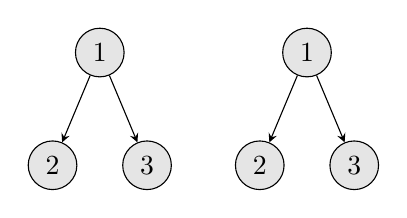
\begin{tikzpicture}
[mynode/.style={draw,circle,minimum size=5mm, fill=gray!20!}]
\node(){};
\node[mynode](1) {1};
\node[mynode](1r) [right = 2cm of 1] {1};
\node[mynode](2) [below = 8mm of 1, xshift=-6mm] {2};
\node[mynode](3) [below = 8mm of 1, xshift=6mm] {3};
\node[mynode](2r) [below = 8mm of 1r, xshift=-6mm] {2};
\node[mynode](3r) [below = 8mm of 1r, xshift=6mm] {3};
\draw[>=stealth,->] (1) -- (2);
\draw[>=stealth,->] (1) -- (3);
\draw[>=stealth,->] (1r) -- (2r);
\draw[>=stealth,->] (1r) -- (3r);
\end{tikzpicture}
\end{figure}
\textbf{Output}: \texttt{true}
\end{flushleft}
\paragraph{Example 2:}
\begin{flushleft}
\textbf{Input}:
\begin{figure}[H]
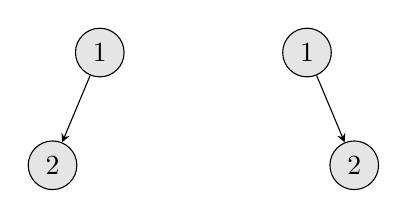
\begin{tikzpicture}
[mynode/.style={draw,circle,minimum size=5mm, fill=gray!20!}]
\node(){};
\node[mynode](1) {1};
\node[mynode](1r) [right = 2cm of 1] {1};
\node[mynode](2) [below = 8mm of 1, xshift=-6mm] {2};
\node[mynode](2r) [below = 8mm of 1r, xshift=6mm] {2};
\draw[>=stealth,->] (1) -- (2);
\draw[>=stealth,->] (1r) -- (2r);
\end{tikzpicture}
\end{figure}
\textbf{Output}: \texttt{false}
\end{flushleft}
\paragraph{Example 3:}
\begin{flushleft}
\textbf{Input}:
\begin{figure}[H]
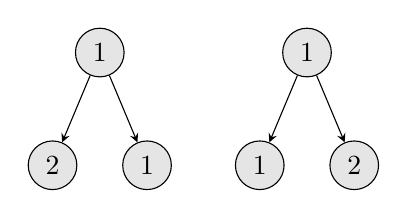
\begin{tikzpicture}
[mynode/.style={draw,circle,minimum size=5mm, fill=gray!20!}]
\node(){};
\node[mynode](1) {1};
\node[mynode](1r) [right = 2cm of 1] {1};
\node[mynode](2) [below = 8mm of 1, xshift=-6mm] {2};
\node[mynode](3) [below = 8mm of 1, xshift=6mm] {1};
\node[mynode](2r) [below = 8mm of 1r, xshift=-6mm] {1};
\node[mynode](3r) [below = 8mm of 1r, xshift=6mm] {2};
\draw[>=stealth,->] (1) -- (2);
\draw[>=stealth,->] (1) -- (3);
\draw[>=stealth,->] (1r) -- (2r);
\draw[>=stealth,->] (1r) -- (3r);
\end{tikzpicture}
\end{figure}
\textbf{Output}: \texttt{false}
\end{flushleft}
\subsection{Recursion}
\begin{CJK*}{UTF8}{gbsn}
很简单的题目,从根节点开始比较,如果都是空节点,返回\texttt{true},如果都是非空节点,先看两个value是否相等,如果不相等,返回\texttt{false},否则recursively比较左子树和右子树即可。
\end{CJK*}
%\section{101 --- Symmetric Tree}
Given a binary tree $T$, check whether it is a mirror of itself (ie, symmetric around its center).
\par
For example, this binary tree is symmetric:
\begin{figure}[H]
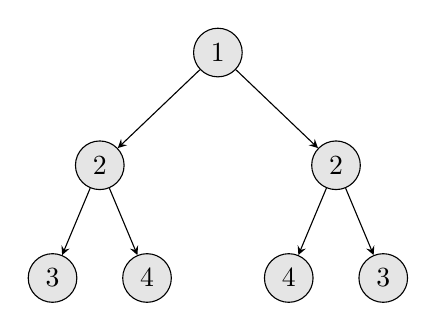
\begin{tikzpicture}
[mynode/.style={draw,circle,minimum size=5mm, fill=gray!20!}]
\node(){};
\node[mynode](1) {1};
\node[mynode](2l) [below = 8mm of 1, xshift=-15mm] {2};
\node[mynode](2r) [below = 8mm of 1, xshift=15mm] {2};
\node[mynode](3l) [below = 8mm of 2l, xshift=-6mm] {3};
\node[mynode](4l) [below = 8mm of 2l, xshift=6mm] {4};
\node[mynode](3r) [below = 8mm of 2r, xshift=6mm] {3};
\node[mynode](4r) [below = 8mm of 2r, xshift=-6mm] {4};
\draw[>=stealth,->] (1) -- (2l);
\draw[>=stealth,->] (1) -- (2r);
\draw[>=stealth,->] (2l) -- (3l);
\draw[>=stealth,->] (2l) -- (4l);
\draw[>=stealth,->] (2r) -- (3r);
\draw[>=stealth,->] (2r) -- (4r);
\end{tikzpicture}
\end{figure}
But the following is not:
\begin{figure}[H]
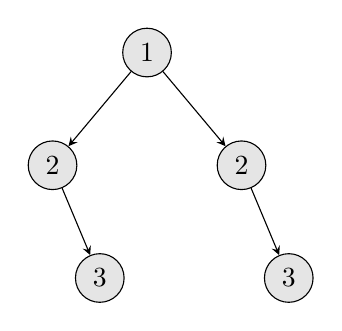
\begin{tikzpicture}
[mynode/.style={draw,circle,minimum size=5mm, fill=gray!20!}]
\node(){};
\node[mynode](1) {1};
\node[mynode](2l) [below = 8mm of 1, xshift=-12mm] {2};
\node[mynode](2r) [below = 8mm of 1, xshift=12mm] {2};
\node[mynode](3l) [below = 8mm of 2l, xshift=6mm] {3};
\node[mynode](3r) [below = 8mm of 2r, xshift=6mm] {3};
\draw[>=stealth,->] (1) -- (2l);
\draw[>=stealth,->] (1) -- (2r);
\draw[>=stealth,->] (2l) -- (3l);
\draw[>=stealth,->] (2r) -- (3r);
\end{tikzpicture}
\end{figure}
\paragraph{Note:}
Bonus points if you could solve it both recursively and iteratively.
\subsection{Recursion}
首先注意到,用于做比较的函数肯定需要两个nodes $n_1$ and $n_2$,因此需要一个额外的辅助函数来进行递归,因为主函数只有一个输入就是根节点。接下来,如果$n_1$ and $n_2$都是空节点,显然是相等的,否则如果都是非空节点并且$n_1$的值和$n_2$的值相等,则递归比较$n_1$的左子树和$n_2$的右子树以及$n_1$的右子树和$n_2$的左子树。
\setcounter{algorithm}{0}
\begin{algorithm}[H]
\caption{Recursion}
\begin{algorithmic}[1]
\Procedure{IsSymmetric}{$T$}
\If{$T=\text{NULL}$}
\State \Return \texttt{true} \Comment Empty node
\EndIf
\State $\texttt{ans}:=\texttt{DFS}(\text{LEFT}(T), \text{RIGHT}(T))$
\algstore{101algo}
\end{algorithmic}
\end{algorithm}
\begin{algorithm}[H]
\begin{algorithmic}[1]
\algrestore{101algo}
\EndProcedure
\end{algorithmic}
\end{algorithm}
\begin{algorithm}[H]
\caption{Recursive Function}
\begin{algorithmic}[1]
\Function{DFS}{$n_1, n_2$}
\If{$n_1=\text{NULL}$ \textbf{and} $n_2=\text{NULL}$}
\State \Return \texttt{true}
\EndIf
\If{$n_1\neq\text{NULL}$ \textbf{and} $n_2\neq\text{NULL}$ \textbf{and} $\text{Value}(n_1)=\text{Value}(n_2)$}
\State $\texttt{ans}:= \texttt{DFS}(\text{LEFT}(n_1), \text{RIGHT}(n_2))$ \Comment Compare left against right
\If{$\texttt{ans}=\texttt{false}$}
\State \Return \texttt{false}
\EndIf
\State $\texttt{ans}\gets \texttt{DFS}(\text{RIGHT}(n_1), \text{LEFT}(n_2))$ \Comment Compare right against left
\State \Return \texttt{ans}
\EndIf
\State \Return \texttt{false}
\EndFunction
\end{algorithmic}
\end{algorithm}
\subsection{Iteration}
这里需要两个queue,一个存放根节点的左子树,另外一个存放根节点的右子树,然后算法基本就和recursion一样。
\begin{algorithm}[H]
\caption{Iteration}
\begin{algorithmic}[1]
\Procedure{IsSymmetric}{$T$}
\If{$T=\text{NULL}$}
\State \Return \texttt{true}
\EndIf
\State Initialize $Q_1$ and $Q_2$ as two empty queues
\State $Q_1\gets Q_1 + \text{LEFT}(T)$
\State $Q_2\gets Q_2 + \text{RIGHT}(T)$
\algstore{102algo}
\end{algorithmic}
\end{algorithm}
\begin{algorithm}[H]
\begin{algorithmic}[1]
\algrestore{102algo}
\While{$Q_1\neq \emptyset$ \textbf{and} $Q_2\neq \emptyset$}
\State $n_1:=\text{FRONT}(Q_1)$
\State $\text{POP}(Q_1)$
\State $n_2:=\text{FRONT}(Q_2)$
\State $\text{POP}(Q_2)$
\If{$n_1=\text{NULL}$ \textbf{and} $n_2=\text{NULL}$}
\State \texttt{continue} \Comment Continue to next items
\EndIf
\If{$n_1\neq\text{NULL}$ \textbf{and} $n_2\neq\text{NULL}$ \textbf{and} $\text{Value}(n_1)=\text{Value}(n_2)$}
\State $Q_1\gets Q_1 + \text{LEFT}(n_1)$
\State $Q_2\gets Q_2 + \text{RIGHT}(n_2)$
\State $Q_1\gets Q_1 + \text{RIGHT}(n_1)$
\State $Q_2\gets Q_2 + \text{LEFT}(n_2)$
\Else
\State \Return \texttt{false}
\EndIf
\EndWhile
\State \Return \texttt{true}
\EndProcedure
\end{algorithmic}
\end{algorithm}
%\section{102 --- Binary Tree Level Order Traversal}
Given a binary tree $T$, return the level order traversal of its nodes' values. (i.e., from left to right, level by level).
\par
For example: Given binary tree
\begin{figure}[H]
\begin{tikzpicture}
[mynode/.style={draw,circle,minimum size=10mm, fill=gray!20!}]
\node(){};
\node[mynode](3) {3};
\node[mynode](9) [below = 8mm of 3, xshift=-10mm] {9};
\node[mynode](20) [below = 8mm of 1, xshift=10mm] {20};
\node[mynode](15) [below = 8mm of 20, xshift=-6mm] {15};
\node[mynode](7) [below = 8mm of 20, xshift=6mm] {7};
\draw[>=stealth,->] (3) -- (9);
\draw[>=stealth,->] (3) -- (20);
\draw[>=stealth,->] (20) -- (15);
\draw[>=stealth,->] (20) -- (7);
\end{tikzpicture}
\end{figure}
return its level order traversal as:
\par
$((3),\ (9,20),\ (15,7))$ 
\subsection{BFS}
Just uses a queue and do BFS search.
%\section{103 --- Binary Tree Zigzag Level Order Traversal}
Given a binary tree $T$, return the zigzag level order traversal of its nodes' values. (ie, from left to right, then right to left for the next level and alternate between). For example: Given binary tree
\begin{figure}[H]
\begin{tikzpicture}
[mynode/.style={draw,circle,minimum size=10mm, fill=gray!20!}]
\node(){};
\node[mynode](3) {3};
\node[mynode](9) [below = 8mm of 3, xshift=-10mm] {9};
\node[mynode](20) [below = 8mm of 1, xshift=10mm] {20};
\node[mynode](15) [below = 8mm of 20, xshift=-6mm] {15};
\node[mynode](7) [below = 8mm of 20, xshift=6mm] {7};
\draw[>=stealth,->] (3) -- (9);
\draw[>=stealth,->] (3) -- (20);
\draw[>=stealth,->] (20) -- (15);
\draw[>=stealth,->] (20) -- (7);
\end{tikzpicture}
\end{figure}
return its zigzag level order traversal as:
\\
$\left((3),\ (20,9),\ (15,7)\right)$
\subsection{BFS}
\begin{CJK*}{UTF8}{gbsn}
同样用BFS搜索,记录每层的节点个数即当前queue的size,然后分奇数偶数层确定访问节点的方向,具体说就是对于奇数层,从右往左,对于偶数层则从左往右,层数从0开始。
\end{CJK*}
%\section{104 --- Maximum Depth of Binary Tree}
Given a binary tree $T$, find its maximum depth.
\par
The maximum depth is the number of nodes along the longest path from the root node down to the farthest leaf node.
\par
Note: A leaf is a node with no children.
\paragraph{Example:}
Given binary tree
\begin{figure}[H]
\begin{tikzpicture}
[mynode/.style={draw,circle,minimum size=10mm, fill=gray!20!}]
\node(){};
\node[mynode](3) {3};
\node[mynode](9) [below = 8mm of 3, xshift=-10mm] {9};
\node[mynode](20) [below = 8mm of 1, xshift=10mm] {20};
\node[mynode](15) [below = 8mm of 20, xshift=-6mm] {15};
\node[mynode](7) [below = 8mm of 20, xshift=6mm] {7};
\draw[>=stealth,->] (3) -- (9);
\draw[>=stealth,->] (3) -- (20);
\draw[>=stealth,->] (20) -- (15);
\draw[>=stealth,->] (20) -- (7);
\end{tikzpicture}
\end{figure}
return its depth $D = 3$.
\subsection{Recursion}
A very easy problem. Just return the maximum depth of left substree and right subtree plus 1 (since we need to count the root).
\subsubsection{Algorithm}
\setcounter{algorithm}{0}
\begin{algorithm}[H]
\caption{Recursion}
\begin{algorithmic}[1]
\Procedure{MaxDepth}{$T$}
\If{$T=\texttt{null}$}
\State \Return 0 \Comment Empty tree has height 1
\EndIf
\State $\alpha:=\texttt{MaxDepth}(\texttt{LEFT}(T))$ \Comment The maximum depth of left subtree
\State $\beta:=\texttt{MaxDepth}(\texttt{RIGHT}(T))$ \Comment The maximum depth of right subtree
\State \Return $1+\max(\alpha, \beta)$
\EndProcedure
\end{algorithmic}
\end{algorithm}
%\section{105 --- Construct Binary Tree from Preorder and Inorder Traversal}\label{105algo}
Given preorder and inorder traversal of a tree, construct the binary tree.
\par
\textbf{Note}: You may assume that duplicates do not exist in the tree.
\par
For example, given
\begin{itemize}
    \item preorder $A = (3,9,20,15,7)$
    \item inorder $B = (9,3,15,20,7)$
\end{itemize}
Return the following binary tree:
\begin{figure}[H]
\begin{tikzpicture}
[mynode/.style={draw,circle,minimum size=10mm, fill=gray!20!}]
\node(){};
\node[mynode](3) {3};
\node[mynode](9) [below = 8mm of 3, xshift=-10mm] {9};
\node[mynode](20) [below = 8mm of 1, xshift=10mm] {20};
\node[mynode](15) [below = 8mm of 20, xshift=-6mm] {15};
\node[mynode](7) [below = 8mm of 20, xshift=6mm] {7};
\draw[>=stealth,->] (3) -- (9);
\draw[>=stealth,->] (3) -- (20);
\draw[>=stealth,->] (20) -- (15);
\draw[>=stealth,->] (20) -- (7);
\end{tikzpicture}
\end{figure}
\subsection{Recursion}
\begin{CJK*}{UTF8}{gbsn}
由于Preorder的第一个肯定是根,所以原二叉树的根节点可以知道,题目中给了一个很关键的条件就是树中没有相同元素,有了这个条件我们就可以在中序遍历中也定位出根节点的位置,并以根节点的位置将中序遍历拆分为左右两个部分,分别对其递归调用原函数。
\par
递归函数必须指定构建二叉树的preorder数组$A$的区间$[p_0, p_1)$和inorder数组$B$的区间$[i_0,i_1)$,然后由于$A[p_0]$就是当前子树的root,因此在$B$中给定的范围顺序搜寻$A[p_0]$在$B$中的位置$\alpha$。找到这个位置后,就知道以$A[p_0]$为root的左子树的长度$L_0:=\alpha - i_0$,右子树的长度$L_1:=i_1 - \alpha - 1$,因此接下来递归建立左子树时,在preroder数组$A$中的搜寻范围是$[p_0+1, p_0+1+L_0)$,相对应的在$B$中的搜寻范围是$[i_0, \alpha)$,而建立右子树时,在$A$中的搜寻范围是$[p_0+L_0+1, p_1)$,在$B$中的搜寻范围是$[\alpha+1, i_1)$
\end{CJK*}
\subsubsection{Algorithm}
\setcounter{algorithm}{0}
\begin{algorithm}[H]
\caption{Recursion}
\begin{algorithmic}[1]
\Procedure{BuildTree}{$A, B, L$}
\State $T:=\texttt{CreateTree}(A, 0, L, B, 0, L)$ \Comment Call \texttt{CreateTree} to create binary tree from $A[0,\ldots, L)$ and $B[0,\ldots,L)$
\State \Return $T$
\EndProcedure
\end{algorithmic}
\end{algorithm}
\begin{CJK*}{UTF8}{gbsn}
\texttt{CreateTree}根据给定的preorder数组$A$和其范围$[p_0, p_1)$以及inorder数组$B$和其范围$[i_0, i_1)$构建出符合要求的binary tree
\end{CJK*}
\begin{algorithm}[H]
\caption{Recursively Building Binary Tree}
\begin{algorithmic}[1]
\Function{CreateTree}{$A, p_0, p_1, B, i_0, i_1$}
\If{$p_0\geq p_1$ \textbf{or} $i_0\geq i_1$} \Comment The ranges are not invalid
\State \Return \texttt{null}
\EndIf
\State $\alpha:=i_0$
\For{$i:=i_0$ \textbf{to} $i_1-1$}
\If{$A[p_0]=B[i]$}
\State $\alpha\gets i$ \Comment Update the root position in $B$
\State \texttt{break} \Comment Stop searching
\EndIf
\EndFor
\State $L_0:=\alpha - i_0$ \Comment The left subtree length
\State $L_1:=i_1 - \alpha - 1$ \Comment The right subtree length
\State Create a new tree node $T$ with root value $A[i_0]$
\State $\texttt{LEFT}(T)\gets \texttt{CreateTree}(A, p_0+1, p_0+L_0+1, B, i_0, \alpha)$ \Comment Create left subtree
\State $\texttt{RIGHT}(T) \gets \texttt{CreateTree}(A, p_0+L_0+1, p_1, B, \alpha+1, i_1)$ \Comment Create right subtree
\State \Return $T$
\EndFunction
\end{algorithmic}
\end{algorithm}
%\section{106 --- Construct Binary Tree from Inorder and Postorder Traversal}
Given inorder and postorder traversal of a tree, construct the binary tree.

\paragraph{Note:}
You may assume that duplicates do not exist in the tree.

For example, given

\fcj{inorder = [9,3,15,20,7]}

\fcj{postorder = [9,15,7,20,3]}

Return the following binary tree:

\begin{figure}[H]
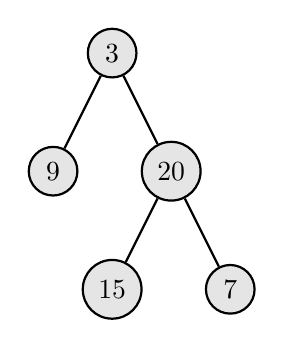
\begin{tikzpicture}
[every node/.style={draw, circle, fill=gray!20!, minimum size=5mm},
%level 1/.style={sibling distance=25mm},
%level 2/.style={sibling distance=15mm},
thick]
\node{3}
child{node{9}}
child{node{20} child{node{15}} child{node{7}}};
\end{tikzpicture}
\end{figure}
%\begin{figure}[H]
%\begin{tikzpicture}
%[mynode/.style={draw,circle,minimum size=10mm, fill=gray!20!}]
%\node(){};
%\node[mynode](3) {3};
%\node[mynode](9) [below = 8mm of 3, xshift=-10mm] {9};
%\node[mynode](20) [below = 8mm of 1, xshift=10mm] {20};
%\node[mynode](15) [below = 8mm of 20, xshift=-6mm] {15};
%\node[mynode](7) [below = 8mm of 20, xshift=6mm] {7};
%\draw[>=stealth,->] (3) -- (9);
%\draw[>=stealth,->] (3) -- (20);
%\draw[>=stealth,->] (20) -- (15);
%\draw[>=stealth,->] (20) -- (7);
%\end{tikzpicture}
%\end{figure}
\subsection{Recursion}
和105基本一样,唯一不同的是root是postorder数组的最后一个元素。递归函数其他部分都是一样的,即求出左子树长度和右子树长度,然后递归构建左子树和右子树。
%\setcounter{algorithm}{0}
%\begin{algorithm}[H]
%\caption{Recursion}
%\begin{algorithmic}[1]
%\Procedure{BuildTree}{$A, B, L$}
%\State $T:=\texttt{CreateTree}(A, 0, L, B, 0, L)$ \Comment Call \texttt{CreateTree} to create binary tree from $A[0,\ldots, L)$ and $B[0,\ldots,L)$
%\State \Return $T$
%\EndProcedure
%\end{algorithmic}
%\end{algorithm}
%\texttt{CreateTree}根据给定的\textbf{postorder}数组$A$和其范围$[p_0, p_1)$以及\textbf{inorder}数组$B$和其范围$[i_0, i_1)$构建出符合要求的binary tree
%\begin{algorithm}[H]
%\caption{Recursively Building Binary Tree}
%\begin{algorithmic}[1]
%\Function{CreateTree}{$A, p_0, p_1, B, i_0, i_1$}
%\If{$p_0\geq p_1$ \textbf{or} $i_0\geq i_1$} \Comment The ranges are not invalid
%\State \Return \texttt{null}
%\EndIf
%\State $\alpha:=i_0$
%\For{$i:=i_0$ \textbf{to} $i_1-1$}
%\If{$A[p_1-1]=B[i]$} \Comment The last element in $A$ is the root
%\State $\alpha\gets i$ \Comment Update the root position in $B$
%\State \texttt{break} \Comment Stop searching
%\EndIf
%\EndFor
%\State $L_0:=\alpha - i_0$ \Comment The left subtree length
%\State $L_1:=i_1 - \alpha - 1$ \Comment The right subtree length
%\State Create a new tree node $T$ with root value $A[i_0]$
%\State $\texttt{LEFT}(T)\gets \texttt{CreateTree}(A, p_0, p_0+L_0, B, i_0, \alpha)$ \Comment Create left subtree
%\State $\texttt{RIGHT}(T) \gets \texttt{CreateTree}(A, p_0+L_0, p_1-1, B, \alpha+1, i_1)$ \Comment Create right subtree
%\State \Return $T$
%\EndFunction
%\end{algorithmic}
%\end{algorithm}
%\section{107 --- Binary Tree Level Order Traversal II}
Given a binary tree, return the \textit{bottom-up level order} traversal of its nodes' values. (i.e, from left to right, level by level from leaf to root).

For example:
Given binary tree \fcj{[3,9,20,null,null,15,7]},

\begin{figure}[H]
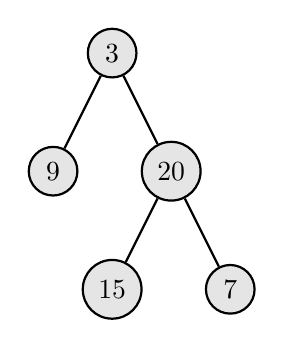
\begin{tikzpicture}
[every node/.style={draw, circle, fill=gray!20!, minimum size=5mm},
%level 1/.style={sibling distance=25mm},
%level 2/.style={sibling distance=15mm},
thick]
\node{3}
child{node{9}}
child{node{20} child{node{15}} child{node{7}}};
\end{tikzpicture}
\end{figure}

return its bottom-up level order traversal as:

\fcj{[ [15,7], [9,20], [3] ]}

\subsection{BFS}
非常容易的题目,用一个queue进行BFS, 然后reverse得到的level遍历数组即可。
%\section{108 --- Convert Sorted Array to Binary Search Tree}
Given an array $A$ where elements are sorted in ascending order, convert it to a height balanced BST.
\par
For this problem, a height-balanced binary tree is defined as a binary tree in which the depth of the two subtrees of every node never differ by more than 1.
\paragraph{Example:}
\begin{flushleft}
\textbf{Input} : $A = (-10,-3,0,5,9)$,
\\
One possible answer is:
\begin{figure}[H]
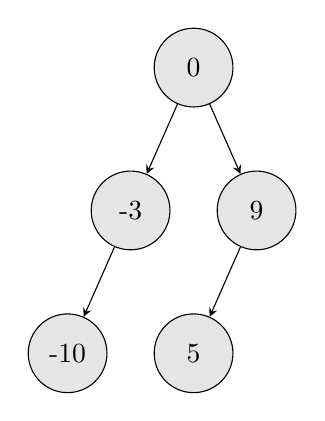
\begin{tikzpicture}
[mynode/.style={draw,circle,minimum size=10mm, fill=gray!20!}]
\node(){};
\node[mynode](0) {0};
\node[mynode](3) [below = 8mm of 0, xshift=-8mm] {-3};
\node[mynode](9) [below = 8mm of 0, xshift=8mm] {9};
\node[mynode](10) [below = 8mm of 3, xshift=-8mm] {-10};
\node[mynode](5) [below = 8mm of 9, xshift=-8mm] {5};
\draw[>=stealth,->] (0) -- (3);
\draw[>=stealth,->] (0) -- (9);
\draw[>=stealth,->] (3) -- (10);
\draw[>=stealth,->] (9) -- (5);
\end{tikzpicture}
\end{figure}
 \end{flushleft}
 \subsection{Recursion}
 \begin{CJK*}{UTF8}{gbsn}
 同样需要一个递归函数制定构建二叉树的范围,首先找到当前范围的中间位置,以中间位置的值作为当前tree的根,然后中间位置往左的部分即为左子树,中间位置往右的部分为右子树。
\end{CJK*}
\subsubsection{Algorithm}
\setcounter{algorithm}{0}
\begin{algorithm}[H]
\caption{Recursion}
\begin{algorithmic}[1]
\Procedure{SortedArrayToBST}{$A, L$}
\State \Return $\texttt{CreateTree}(A, 0, L-1)$ \Comment Create BST for $A[0,\ldots, L-1]$
\EndProcedure
\end{algorithmic}
\end{algorithm}
\begin{CJK*}{UTF8}{gbsn}
\texttt{CreateTree}根据给定的有序数组$A$及其范围$[\alpha, \beta]$构建出一个二叉搜索树
\end{CJK*}
\begin{algorithm}[H]
\caption{Recursively Build Binary Search Tree}
\begin{algorithmic}[1]
\Function{CreateTree}{$A, \alpha, \beta$}
\If{$\alpha > \beta$}
\State \Return \texttt{null}
\EndIf
\State $M:=(\alpha+\beta)/2$ \Comment The midpoint
\State Create tree node $T$ with value equal to $A[M]$
\State $\texttt{LEFT}(T)\gets \texttt{CreateTree}(A, \alpha, M-1)$ \Comment Build left child tree for $A[\alpha, M-1]$
\State $\texttt{RIGHT}(T)\gets \texttt{CreateTree}(A, M+1, \beta)$ \Comment Build right child tree for $A[M+1, \beta]$
\State \Return $T$
\EndFunction 
\end{algorithmic}
\end{algorithm}
%\section{109 --- Convert Sorted List to Binary Search Tree}
Given a singly linked list $L$ where elements are sorted in ascending order, convert it to a height balanced BST.
\par
For this problem, a height-balanced binary tree is defined as a binary tree in which the depth of the two subtrees of every node never differ by more than 1.
\paragraph{Example:}
\begin{flushleft}
\textbf{Input}: $L = [-10,-3,0,5,9]$,
\\
One possible answer is:
\begin{figure}[H]
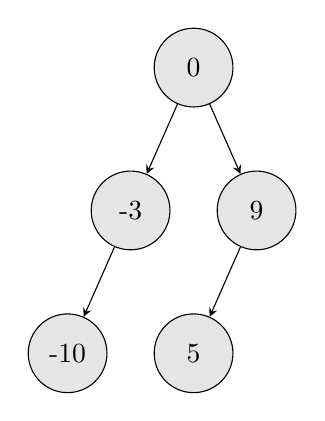
\begin{tikzpicture}
[mynode/.style={draw,circle,minimum size=10mm, fill=gray!20!}]
\node(){};
\node[mynode](0) {0};
\node[mynode](3) [below = 8mm of 0, xshift=-8mm] {-3};
\node[mynode](9) [below = 8mm of 0, xshift=8mm] {9};
\node[mynode](10) [below = 8mm of 3, xshift=-8mm] {-10};
\node[mynode](5) [below = 8mm of 9, xshift=-8mm] {5};
\draw[>=stealth,->] (0) -- (3);
\draw[>=stealth,->] (0) -- (9);
\draw[>=stealth,->] (3) -- (10);
\draw[>=stealth,->] (9) -- (5);
\end{tikzpicture}
\end{figure}
 \end{flushleft}
 \subsection{Recursion}
 \begin{CJK*}{UTF8}{gbsn}
 链表的查找中间点可以通过快慢指针来操。找到中点后,要以中点的值建立一个根节点,然后需要把原链表断开,分为前后两个链表,都不能包含原中点,然后再分别对这两个链表递归调用原函数,分别连上左右子节点即可。因此,仍然需要一个辅助函数来进行递归操作,这个辅助函数有两个输入参数,即起始节点和尾部节点后的第一个节点。
\end{CJK*}
\subsubsection{Algorithm}
\setcounter{algorithm}{0}
\begin{algorithm}[H]
\caption{Recursion}
\begin{algorithmic}[1]
\Procedure{SortedListToBST}{$L$}
\If{$L=\texttt{null}$}
\State \Return \texttt{null}
\EndIf
\State $T:=\texttt{CreateTree}(L, \texttt{null})$
\EndProcedure
\end{algorithmic}
\end{algorithm}
 \begin{CJK*}{UTF8}{gbsn}
 \texttt{CreateTree}根据输入的起始节点$\alpha$和尾部节点后的第一个节点$\beta$构建二叉搜索树
\end{CJK*}
\begin{algorithm}[H]
\caption{Recursively Build Binary Search Tree}
\begin{algorithmic}[1]
\Function{CreateTree}{$\alpha, \beta$}
\If{$\alpha=\beta$} \Comment Cannot compare larger/smaller for linked list nodes
\State \Return \texttt{null}
\EndIf
\State $F:=\alpha$ \Comment Fast pointer
\State $S:=\alpha$ \Comment Slow pointer
\While{$\texttt{Next}(F)\neq \beta$ \textbf{and} $\texttt{Next}(\texttt{Next}(F))\neq \beta$ }
\State $F\gets \texttt{Next}(\texttt{Next}(F))$ \Comment Forward fast pointer by 2 nodes
\State $S\gets \texttt{Next}(S)$ \Comment Forward slow pointer by 1 node
\EndWhile
\State Create a tree node $T$ with value equal to $\texttt{Value}(S)$ 
\State $\texttt{LEFT}(T)\gets \texttt{CreateTree}(\alpha, S)$ \Comment Create left subtree
\State $\texttt{RIGHT}(T)\gets \texttt{CreateTree}(\texttt{Next}(S), \beta)$ \Comment Create right subtree
\State \Return $T$
\EndFunction
\end{algorithmic}
\end{algorithm} 
%\section{110 --- Balanced Binary Tree}
Given a binary tree $T$, determine if it is height-balanced.
\par
For this problem, a height-balanced binary tree is defined as: a binary tree in which the depth of the two subtrees of every node never differ by more than 1.
\paragraph{Example 1:}
\begin{flushleft}
\textbf{Input}
\begin{figure}[H]
\begin{tikzpicture}
[mynode/.style={draw,circle,minimum size=10mm, fill=gray!20!}]
\node(){};
\node[mynode](3) {3};
\node[mynode](9) [below = 8mm of 3, xshift=-10mm] {9};
\node[mynode](20) [below = 8mm of 1, xshift=10mm] {20};
\node[mynode](15) [below = 8mm of 20, xshift=-6mm] {15};
\node[mynode](7) [below = 8mm of 20, xshift=6mm] {7};
\draw[>=stealth,->] (3) -- (9);
\draw[>=stealth,->] (3) -- (20);
\draw[>=stealth,->] (20) -- (15);
\draw[>=stealth,->] (20) -- (7);
\end{tikzpicture}
\end{figure}
\textbf{Output}: \texttt{true}
\end{flushleft}
\paragraph{Example 2:}
\begin{flushleft}
\textbf{Input}:
\begin{figure}[H]
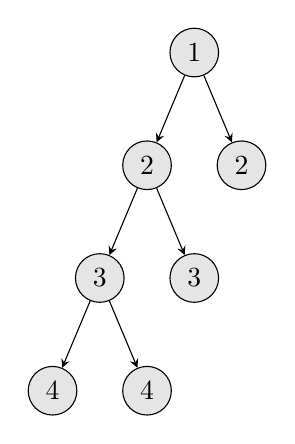
\begin{tikzpicture}
[mynode/.style={draw,circle,minimum size=5mm, fill=gray!20!}]
\node(){};
\node[mynode](1) {1};
\node[mynode](2l) [below = 8mm of 1, xshift=-6mm] {2};
\node[mynode](2r) [below = 8mm of 1, xshift=6mm] {2};
\node[mynode](3l) [below = 8mm of 2l, xshift=-6mm] {3};
\node[mynode](3r) [below = 8mm of 2l, xshift=6mm] {3};
\node[mynode](4l) [below = 8mm of 3l, xshift=-6mm] {4};
\node[mynode](4r) [below = 8mm of 3l, xshift=6mm] {4};
\draw[>=stealth,->] (1) -- (2l);
\draw[>=stealth,->] (1) -- (2r);
\draw[>=stealth,->] (2l) -- (3l);
\draw[>=stealth,->] (2l) -- (3r);
\draw[>=stealth,->] (3l) -- (4l);
\draw[>=stealth,->] (3l) -- (4r);
\end{tikzpicture}
\end{figure}
\textbf{Output}: \texttt{false}
 \end{flushleft}
 \subsection{Recursion}
根据题目中的定义,高度平衡二叉树是每一个结点的两个子树的深度差不能超过1,那么肯定需要一个求各个点深度的函数,然后对每个节点的两个子树来比较深度差,但是这种方法效率差,因为每一个点都会被上面的点计算深度时访问一次,优化后的方法是如果我们发现子树不平衡,则不计算具体的深度,而是直接返回-1。那么优化后的方法为:对于每一个节点,递归获得左右子树的深度,如果子树是平衡的,则返回真实的深度,若不平衡,直接返回$-1$
\setcounter{algorithm}{0}
\begin{algorithm}[H]
\caption{Recursion}
\begin{algorithmic}[1]
\Procedure{IsBalanced}{$T$}
\If{$\texttt{MaxDepth} < 0$}
\State \Return \texttt{false}
\EndIf
\State \Return \texttt{true}
\EndProcedure
\end{algorithmic}
\end{algorithm}
\begin{CJK*}{UTF8}{gbsn}
\texttt{MaxDepth} 在计算每个节点的最大深度时,同时进行左右子树深度的比较,如果深度大于1,返回$-1$,否则返回实际的最大深度。
\end{CJK*}
\begin{algorithm}[H]
\caption{Include Balance Check In Computing Maximum Depth}
\begin{algorithmic}[1]
\Function{MaxDepth}{$T$}
\If{$T=\texttt{null}$}
\State \Return 0
\EndIf
\State $\alpha:=\texttt{MaxDepth}(\texttt{LEFT}(T))$ \Comment The maximum depth of left subtree
\If{$\alpha < 0$} \Comment Left subtree is unbalanced
\State \Return $-1$
\EndIf
\State $\beta:=\texttt{MaxDepth}(\texttt{RIGHT}(T))$ \Comment The maximum depth of right subtree
\If{$\beta < 0$} \Comment Left subtree is unbalanced
\State \Return $-1$
\EndIf
\State $d:=|\alpha-\beta|$ \Comment The absolute difference
\If{$d > 1$}
\State \Return $-1$ \Comment $T$ is unbalanced
\EndIf
\State \Return $1+\max(l, r)$ \Comment $T$ is balanced so return the actual maximum depth
\algstore{110algo}
\end{algorithmic}
\end{algorithm}
\begin{algorithm}[H]
\begin{algorithmic}[1]
\algrestore{110algo}
\EndFunction
\end{algorithmic}
\end{algorithm}
%\section{111 --- Minimum Depth of Binary Tree}
Given a binary tree, find its minimum depth.

The minimum depth is the number of nodes along the shortest path from the root node down to the nearest leaf node.

\textbf{Note}: A leaf is a node with no children.

\paragraph{Example:}
\begin{flushleft}

Given binary tree \fcj{[3,9,20,null,null,15,7]},

\begin{figure}[H]

\begin{figure}[H]
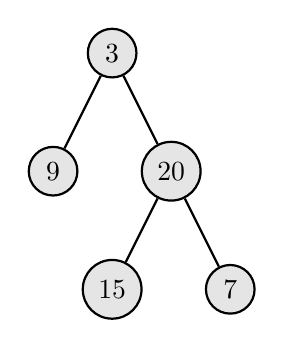
\begin{tikzpicture}
[every node/.style={draw, circle, fill=gray!20!, minimum size=5mm},
%level 1/.style={sibling distance=25mm},
%level 2/.style={sibling distance=15mm},
thick]
\node{3}
child{node{9}}
child{node{20} child{node{15}} child{node{7}}};
\end{tikzpicture}
\end{figure}

\end{figure}
return its minimum \fcj{depth = 2}.
\end{flushleft}

\subsection{Depth First Search}
We incorporate find balance into calculate depth. If we find each node has unbalanced left and right child tree, we return a negative number.

\setcounter{lstlisting}{0}
\begin{lstlisting}[style=customc, caption={DFS}]
bool isBalanced( TreeNode* root )
{
    auto res = depth( root );
    return res >= 0;
}
//helper function to find depth of a node
//we incorprate into comparing depth of left and right
//child tree
//when it is not balance,
//return -1
int depth( TreeNode* node )
{
    if( !node )
    {
        return 0;
    }
    int l_dep = depth( node->left );
    if( l_dep < 0 )
    {
        return -1;
    }

    int r_dep = depth( node->right );
    if( r_dep < 0 )
    {
        return -1;
    }
    //check if left and right child tree
    //are balanced
    int diff = abs( l_dep - r_dep );
    if( diff > 1 )
    {
        //unbalanced
        return -1;
    }
    //balanced
    //return the depth
    return ( max )( l_dep, r_dep ) + 1;
}
\end{lstlisting}

%\section{112 --- Path Sum}
Given a binary tree $T$ and a sum $S$, determine if the tree has a root-to-leaf path such that adding up all the values along the path equals the given sum.
\par
Note: A leaf is a node with no children.
\paragraph{Example:}
\begin{flushleft}
\textbf{Input}: $S=22$, $T$ is given below
\begin{figure}[H]
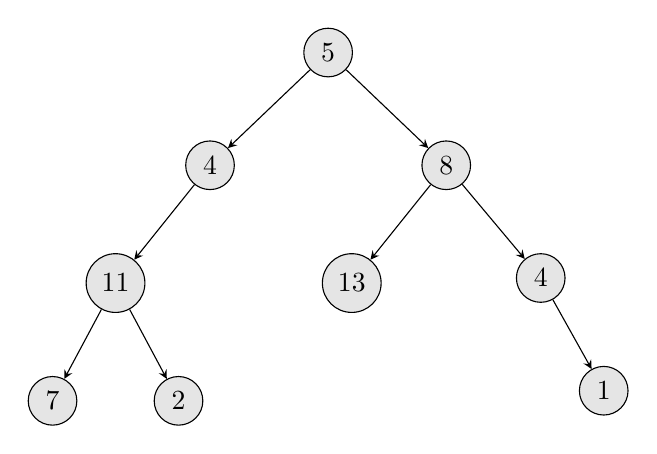
\begin{tikzpicture}
[mynode/.style={draw,circle,minimum size=5mm, fill=gray!20!}]
\node(){};
\node[mynode](5) {5};
\node[mynode](4) [below = 8mm of 5, xshift=-15mm] {4};
\node[mynode](8) [below = 8mm of 5, xshift=15mm] {8};
\node[mynode](11) [below = 8mm of 4, xshift=-12mm] {11};
\node[mynode](13) [below = 8mm of 8, xshift=-12mm] {13};
\node[mynode](41) [below = 8mm of 8, xshift=12mm] {4};
\node[mynode](7) [below = 8mm of 11, xshift=-8mm] {7};
\node[mynode](2) [below = 8mm of 11, xshift=8mm] {2};
\node[mynode](1) [below = 8mm of 41, xshift=8mm] {1};
\draw[>=stealth,->] (5) -- (4);
\draw[>=stealth,->] (5) -- (8);
\draw[>=stealth,->] (4) -- (11);
\draw[>=stealth,->] (8) -- (13);
\draw[>=stealth,->] (8) -- (41);
\draw[>=stealth,->] (11) -- (7);
\draw[>=stealth,->] (11) -- (2);
\draw[>=stealth,->] (41) -- (1);
\end{tikzpicture}
\end{figure}
\textbf{Output}: \texttt{true}, as there exist a root-to-leaf path $5\to4\to11\to2$ which sum is 22.
\end{flushleft}
\subsection{Recursive}
递归方法是最直接想到的方法:如果当前节点是空节点,显然是\texttt{false}。
\begin{itemize}
    \item 如果当前node是leaf,看其值是否与$S$相等,相等返回\texttt{true},否则\texttt{false}。
    \item 如果不是leaf,首先递归处理left subtree,如果结果找到,返回\texttt{true},否则递归处理right subtree,返回处理结果。
\end{itemize}

\setcounter{lstlisting}{0}
\begin{lstlisting}[style=customc, caption={Recursion}]
bool hasPathSum( TreeNode* root, int sum )
{
    if( !root )
    {
        //empty node
        return false;
    }
    if( !root->left && !root->right )
    {
        //leaf node
        return root->val == sum;
    }
    //check if the path exists in left child tree
    if( !hasPathSum( root->left, sum - root->val ) )
    {
        //check if the path exists in right child tree
        return hasPathSum( root->right, sum - root->val );
    }
    return true;
}
\end{lstlisting}
%\section{113 --- Path Sum II}
Given a binary tree $T$ and a sum $S$, find all root-to-leaf paths where each path's sum equals the given sum.
\par
Note: A leaf is a node with no children.
\par
\paragraph{Example:}
\begin{flushleft}
\textbf{Input}: $S=22$, $T$ is given as below
\begin{figure}[H]
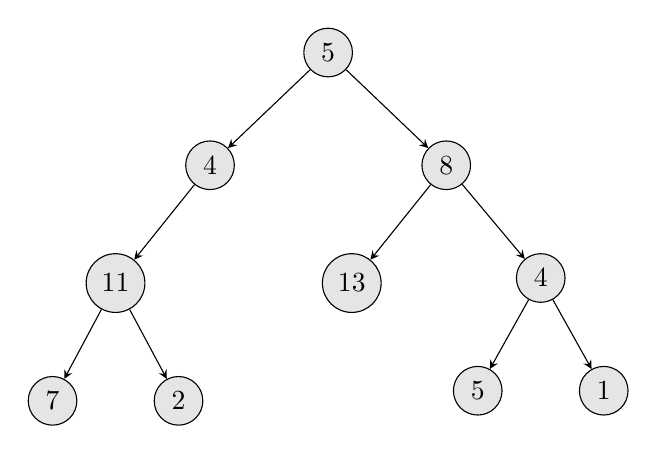
\begin{tikzpicture}
[mynode/.style={draw,circle,minimum size=5mm, fill=gray!20!}]
\node(){};
\node[mynode](5) {5};
\node[mynode](4) [below = 8mm of 5, xshift=-15mm] {4};
\node[mynode](8) [below = 8mm of 5, xshift=15mm] {8};
\node[mynode](11) [below = 8mm of 4, xshift=-12mm] {11};
\node[mynode](13) [below = 8mm of 8, xshift=-12mm] {13};
\node[mynode](41) [below = 8mm of 8, xshift=12mm] {4};
\node[mynode](7) [below = 8mm of 11, xshift=-8mm] {7};
\node[mynode](2) [below = 8mm of 11, xshift=8mm] {2};
\node[mynode](1) [below = 8mm of 41, xshift=8mm] {1};
\node[mynode](51) [below = 8mm of 41, xshift=-8mm] {5};
\draw[>=stealth,->] (5) -- (4);
\draw[>=stealth,->] (5) -- (8);
\draw[>=stealth,->] (4) -- (11);
\draw[>=stealth,->] (8) -- (13);
\draw[>=stealth,->] (8) -- (41);
\draw[>=stealth,->] (11) -- (7);
\draw[>=stealth,->] (11) -- (2);
\draw[>=stealth,->] (41) -- (1);
\draw[>=stealth,->] (41) -- (51);
\end{tikzpicture}
\end{figure}
\textbf{Output}:
\\
$(5,4,11,2)$
\\
$(5,8,4,5)$
\end{flushleft}
\subsection{Recursion}
\begin{CJK*}{UTF8}{gbsn}
由于需要保存路径,因此每次进入到递归函数时,将当前node的值插入到当前path的末尾,然后在递归结束时,将末尾的node从path中移除。
\end{CJK*}
\subsubsection{Algorithm}
\setcounter{algorithm}{0}
\begin{algorithm}[H]
\caption{Depth First Search}
\begin{algorithmic}[1]
\Procedure{PathSum}{$T, S$}
\State $\texttt{ans}:=\emptyset$ \Comment The path collections
\State $P:=\emptyset$ \Comment The path array
\State $\texttt{DFS}(T, S, P, \texttt{ans})$
\State \Return \texttt{ans}
\EndProcedure
\end{algorithmic}
\end{algorithm}
\begin{CJK*}{UTF8}{gbsn}
\texttt{DFS}从给定的二叉树$T$中找到所有的路径和等于$S$的path。
\end{CJK*}
\begin{algorithm}[H]
\caption{Help Function To Do Depth First Search}
\begin{algorithmic}[1]
\Function{DFS}{$T, S, P, A$}
\If{$T=\texttt{null}$}
\State \Return
\EndIf
\If{$\texttt{Left}(T)=\texttt{null}$ \textbf{and} $\texttt{Right}(T)=\texttt{null}$}
\If{$S=\texttt{Value}(T)$}
\State $P\gets P + \texttt{Value}(T)$ \Comment Add to current path
\State $A\gets A +  P$ \Comment Add this path to the path collection
\State $P\gets P\setminus P[-1]$ \Comment Remove end element from $P$
\EndIf
\State \Return  \Comment Exit current recursion
\EndIf
\State $P\gets P + \texttt{Value}(T)$ \Comment Add to current path
\State $\texttt{DFS}(\texttt{Left}(T), S - \texttt{Value}(T), P, A)$ \Comment Recursive on left subtree
\State $\texttt{DFS}(\texttt{Right}(T), S - \texttt{Value}(T), P, A)$ \Comment Recursive on right subtree
\State $P\gets P\setminus P[-1]$ \Comment Remove end element from $P$
\EndFunction
\end{algorithmic}
\end{algorithm}
%\section{114 --- Flatten Binary Tree to Linked List}
Given a binary tree $T$, flatten it to a linked list in-place.
\par
For example, given the following tree:
\begin{figure}[H]
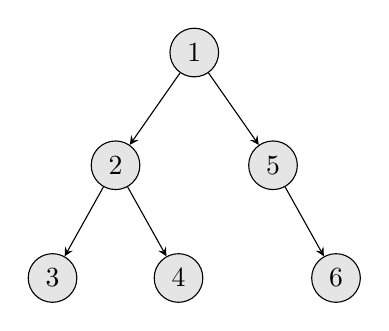
\begin{tikzpicture}
[mynode/.style={draw,circle,minimum size=5mm, fill=gray!20!}]
\node(){};
\node[mynode](1) {1};
\node[mynode](2) [below = 8mm of 1, xshift=-10mm] {2};
\node[mynode](5) [below = 8mm of 1, xshift=10mm] {5};
\node[mynode](3) [below = 8mm of 2, xshift=-8mm] {3};
\node[mynode](4) [below = 8mm of 2, xshift=8mm] {4};
\node[mynode](6) [below = 8mm of 5, xshift=8mm] {6};
\draw[>=stealth,->] (1) -- (2);
\draw[>=stealth,->] (1) -- (5);
\draw[>=stealth,->] (2) -- (3);
\draw[>=stealth,->] (2) -- (4);
\draw[>=stealth,->] (5) -- (6);
\end{tikzpicture}
\end{figure}
The flattened tree should look like:
\begin{figure}[H]
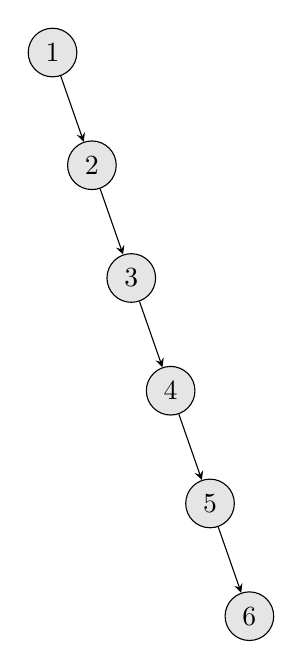
\begin{tikzpicture}
[mynode/.style={draw,circle,minimum size=5mm, fill=gray!20!}]
\node(){};
\node[mynode](1) {1};
\node[mynode](2) [below = 8mm of 1, xshift=5mm] {2};
\node[mynode](3) [below = 8mm of 2, xshift=5mm] {3};
\node[mynode](4) [below = 8mm of 3, xshift=5mm] {4};
\node[mynode](5) [below = 8mm of 4, xshift=5mm] {5};
\node[mynode](6) [below = 8mm of 5, xshift=5mm] {6};
\draw[>=stealth,->] (1) -- (2);
\draw[>=stealth,->] (2) -- (3);
\draw[>=stealth,->] (3) -- (4);
\draw[>=stealth,->] (4) -- (5);
\draw[>=stealth,->] (5) -- (6);
\end{tikzpicture}
\end{figure}
\subsection{Depth First Search}
根据展开后形成的链表的顺序分析出是使用preorder traverse,如果用recursive depth first search,那么首先对左右子树分别进行flatten,接着保存当前节点的右子树,然后将当前节点的右子树替换成左子树,然后把当前节点的左子树设为\texttt{nullptr},接着,沿着新的右子树(其实就是之前的左子树)的right一直走到叶子节点,然后将这个叶子节点的右子树设为之前保存的原来的右子树。

而对于iterative方法,则从root开始出发,先检测root的left node是否存在,如存在则将root和其right node断开,将left node及其子树一起连到原right node的位置,然后再把原right node连到原来的left node最右面的right node之后
\setcounter{lstlisting}{0}
\begin{lstlisting}[style=customc, caption={Recursion}]
void flatten( TreeNode* root )
{
    if( !root )
    {
        return;
    }
    //flatten left child
    flatten( root->left );
    //flatten right child
    flatten( root->right );
    //save current right child first
    auto x = root->right;
    //move left child to right child
    root->right = root->left;
    root->left = nullptr;
    //link to previous right child
    auto node = root;
    while( node->right )
    {
        node = node->right;
    }
    node->right = x;
}
\end{lstlisting}
The process of transformation of the given example is shown as below:
\begin{figure}[H]
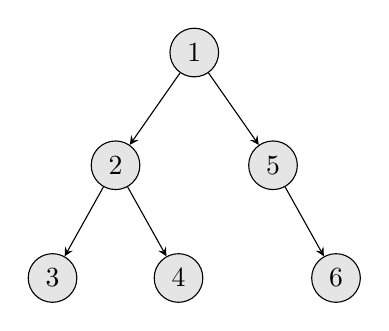
\begin{tikzpicture}
[mynode/.style={draw,circle,minimum size=5mm, fill=gray!20!}]
\node(){};
\node[mynode](1) {1};
\node[mynode](2) [below = 8mm of 1, xshift=-10mm] {2};
\node[mynode](5) [below = 8mm of 1, xshift=10mm] {5};
\node[mynode](3) [below = 8mm of 2, xshift=-8mm] {3};
\node[mynode](4) [below = 8mm of 2, xshift=8mm] {4};
\node[mynode](6) [below = 8mm of 5, xshift=8mm] {6};
\draw[>=stealth,->] (1) -- (2);
\draw[>=stealth,->] (1) -- (5);
\draw[>=stealth,->] (2) -- (3);
\draw[>=stealth,->] (2) -- (4);
\draw[>=stealth,->] (5) -- (6);
\end{tikzpicture}
\caption{Original Tree}
\end{figure}
\begin{figure}[H]
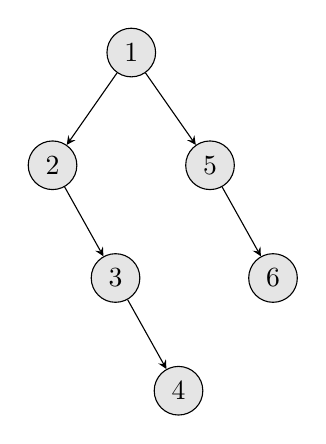
\begin{tikzpicture}
[mynode/.style={draw,circle,minimum size=5mm, fill=gray!20!}]
\node(){};
\node[mynode](1) {1};
\node[mynode](2) [below = 8mm of 1, xshift=-10mm] {2};
\node[mynode](5) [below = 8mm of 1, xshift=10mm] {5};
\node[mynode](3) [below = 8mm of 2, xshift=8mm] {3};
\node[mynode](4) [below = 8mm of 3, xshift=8mm] {4};
\node[mynode](6) [below = 8mm of 5, xshift=8mm] {6};
\draw[>=stealth,->] (1) -- (2);
\draw[>=stealth,->] (1) -- (5);
\draw[>=stealth,->] (2) -- (3);
\draw[>=stealth,->] (3) -- (4);
\draw[>=stealth,->] (5) -- (6);
\end{tikzpicture}
\caption{Recursive On Left And Right Subtree}
\end{figure}
\begin{figure}[H]
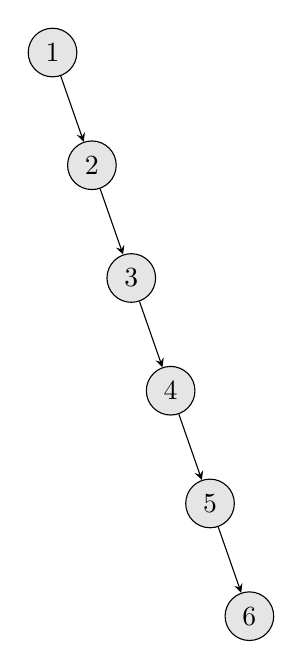
\begin{tikzpicture}
[mynode/.style={draw,circle,minimum size=5mm, fill=gray!20!}]
\node(){};
\node[mynode](1) {1};
\node[mynode](2) [below = 8mm of 1, xshift=5mm] {2};
\node[mynode](3) [below = 8mm of 2, xshift=5mm] {3};
\node[mynode](4) [below = 8mm of 3, xshift=5mm] {4};
\node[mynode](5) [below = 8mm of 4, xshift=5mm] {5};
\node[mynode](6) [below = 8mm of 5, xshift=5mm] {6};
\draw[>=stealth,->] (1) -- (2);
\draw[>=stealth,->] (2) -- (3);
\draw[>=stealth,->] (3) -- (4);
\draw[>=stealth,->] (4) -- (5);
\draw[>=stealth,->] (5) -- (6);
\end{tikzpicture}
\caption{Replace Right By Left Subtree}
\end{figure}

The following is the implementation of iterative way

\begin{lstlisting}[style=customc, caption={Iterative Approach}]
void flatten( TreeNode* root )
{
    auto node = root;
    while( node )
    {
        if( node->left )
        {
            auto t = node->left;
            //get the rightmost node of left child
            while( t->right )
            {
                t = t->right;
            }
            //link to current node's right child
            t->right = node->right;
            node->right = node->left;
            node->left = nullptr;
        }
        node = node->right; //move to right child
    }
}
\end{lstlisting}
The process of transformation for the given example tree is shown as below
\begin{figure}[H]
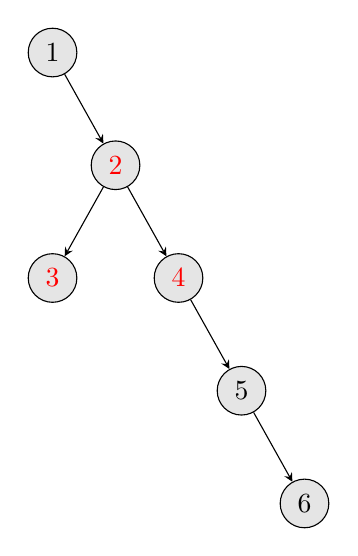
\begin{tikzpicture}
[mynode/.style={draw,circle,minimum size=5mm, fill=gray!20!}]
\node(){};
\node[mynode](1) {1};
\node[mynode](2) [below = 8mm of 1, xshift=8mm] {\textcolor{red}{2}};
\node[mynode](3) [below = 8mm of 2, xshift=-8mm] {\textcolor{red}{3}};
\node[mynode](4) [below = 8mm of 2, xshift=8mm] {\textcolor{red}{4}};
\node[mynode](5) [below = 8mm of 4, xshift=8mm] {5};
\node[mynode](6) [below = 8mm of 5, xshift=8mm] {6};
\draw[>=stealth,->] (1) -- (2);
\draw[>=stealth,->] (2) -- (3);
\draw[>=stealth,->] (2) -- (4);
\draw[>=stealth,->] (4) -- (5);
\draw[>=stealth,->] (5) -- (6);
\end{tikzpicture}
\caption{Change Left And Right Subtree}
\end{figure}
\begin{figure}[H]
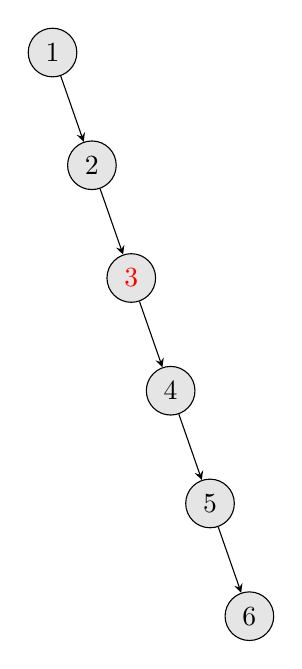
\begin{tikzpicture}
[mynode/.style={draw,circle,minimum size=5mm, fill=gray!20!}]
\node(){};
\node[mynode](1) {1};
\node[mynode](2) [below = 8mm of 1, xshift=5mm] {2};
\node[mynode](3) [below = 8mm of 2, xshift=5mm] {\textcolor{red}{3}};
\node[mynode](4) [below = 8mm of 3, xshift=5mm] {4};
\node[mynode](5) [below = 8mm of 4, xshift=5mm] {5};
\node[mynode](6) [below = 8mm of 5, xshift=5mm] {6};
\draw[>=stealth,->] (1) -- (2);
\draw[>=stealth,->] (2) -- (3);
\draw[>=stealth,->] (3) -- (4);
\draw[>=stealth,->] (4) -- (5);
\draw[>=stealth,->] (5) -- (6);
\end{tikzpicture}
\caption{The Final Result}
\end{figure}
%\section{115 --- Distinct Subsequences}
Given a string $S$ and a string $T$, count the number of distinct subsequences of $S$ which equals $T$.
\par
A subsequence of a string is a new string which is formed from the original string by deleting some (can be none) of the characters without disturbing the relative positions of the remaining characters. (i.e, \texttt{ACE} is a subsequence of \texttt{ABCDE} while \texttt{AEC} is not).
\paragraph{Example 1:}
\begin{flushleft}
\textbf{Input}: $S = \texttt{rabbbit}$, $T = \texttt{rabbit}$
\\
\textbf{Output}: 3
\\
\textbf{Explanation}:
\\
As shown below, there are 3 ways you can generate \texttt{rabbit} from $S$.
\begin{itemize}
    \item \textbf{rabb}b\textbf{it}
    \item \textbf{ra}b\textbf{bbit}
    \item \textbf{rab}b\textbf{bit}
\end{itemize}
\end{flushleft}
\paragraph{Example 2:}
\begin{flushleft}
\textbf{Input}: $S = \texttt{babgbag}$,  $T = \texttt{bag}$
\\
\textbf{Output}: 5
\\
\textbf{Explanation}:
\\
As shown below, there are 5 ways you can generate \texttt{bag} from $S$.
\begin{itemize}
    \item \textbf{ba}b\textbf{g}bag
    \item \textbf{ba}bgba\textbf{g}
    \item \textbf{b}abgb\textbf{ag}
    \item ba\textbf{b}gb\textbf{ag}
    \item babg\textbf{bag}
    \end{itemize}
\end{flushleft}
\subsection{Dynamic Programming}
\begin{CJK*}{UTF8}{gbsn}
这种问题一般依靠Dynamic Programming来解决,假设$F[i][j]$表示$S[0,i-1]$中能够表示$T[0,j-1]$的subsequence的个数,$i=0$或者$j=0$则表示$S[0,-1]$或者$T[0,-1]$是空字符串。很显然$F[i][0]=1$因为对于$T$为空字符串,$S$中只有一个subsequence也就是空字符串能表示空字符串。对于$i>0$ and $j>0$,首先$F[i][j] = 0 + F[i-1][j]$即首先要加上$S[0,i-2]$中能够表示$T[0,j-1]$的subsequence的个数,接着看$S[i-1]$是否和$T[j-1]$相等,如果相等,$F[i][j]$还要加上$F[i-1][j-1]$,即$S[0,i-2]$中能够表示$T[0,j-2]$的subsequence的个数。不相等就不用加了。
\end{CJK*}
\setcounter{algorithm}{0}
\begin{algorithm}[H]
\caption{Dynamic Programming}
\begin{algorithmic}[1]
\Procedure{NumDistinct}{$S,\;L_S,\;T,\;L_T$}
\State Initialize DP array $F[i][j]$
\State $F[0][0]=\ldots=F[L_S+1][L_T+1]:=0$
\For{$x:=0 \to L_S$}
\State $F[x][0]\gets 1$ \Comment Empty string only has one way to represent
\EndFor
\For{$x:=1 \to L_S$}
\For{$y:=1 \to L_T$}
\State $F[x][y]\gets F[x-1][y]$ 
\If{$S[x-1]=T[y-1]$}
\State $F[x][y]\gets F[x][y] + F[x-1][y-1]$
\EndIf
\EndFor
\EndFor
\State \Return $F[L_S][L_T]$
\EndProcedure
\end{algorithmic}
\end{algorithm}


%\definecolor{mygreen}{rgb}{0,0.6,0}
\definecolor{mygray}{rgb}{0.5,0.5,0.5}
\definecolor{mymauve}{rgb}{0.58,0,0.82}

\section{116 --- Populating Next Right Pointers in Each Node}
Given a binary tree $T$

\begin{lstlisting}[style=customc]
struct TreeLinkNode {
  TreeLinkNode *left;
  TreeLinkNode *right;
  TreeLinkNode *next;
}
\end{lstlisting}
Populate each next pointer to point to its next right node. If there is no next right node, the next pointer should be set to \texttt{null}.
\par
Initially, all next pointers are set to \texttt{null}.
\paragraph{Note:}
\begin{itemize}
    \item You may only use constant extra space.
    \item Recursive approach is fine, implicit stack space does not count as extra space for this problem.
    \item You may assume that it is a perfect binary tree (i.e., all leaves are at the same level, and every parent has two children).
\end{itemize}
\paragraph{Example:}
\begin{flushleft}
\textbf{Input}
\begin{figure}[H]
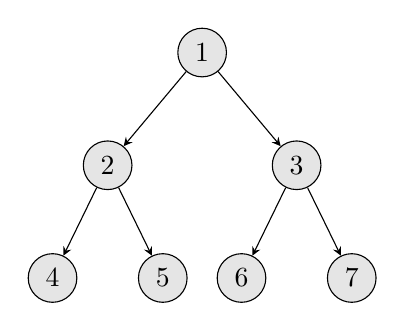
\begin{tikzpicture}
[mynode/.style={draw,circle,minimum size=5mm, fill=gray!20!}]
\node(){};
\node[mynode](1) {1};
\node[mynode](2) [below = 8mm of 1, xshift=-12mm] {2};
\node[mynode](3) [below = 8mm of 1, xshift=12mm] {3};
\node[mynode](4) [below = 8mm of 2, xshift=-7mm] {4};
\node[mynode](5) [below = 8mm of 2, xshift=7mm] {5};
\node[mynode](6) [below = 8mm of 3, xshift=-7mm] {6};
\node[mynode](7) [below = 8mm of 3, xshift=7mm] {7};
\draw[>=stealth,->] (1) -- (2);
\draw[>=stealth,->] (1) -- (3);
\draw[>=stealth,->] (2) -- (4);
\draw[>=stealth,->] (2) -- (5);
\draw[>=stealth,->] (3) -- (6);
\draw[>=stealth,->] (3) -- (7);
\end{tikzpicture}
\end{figure}
\textbf{Output}:
\begin{figure}[H]
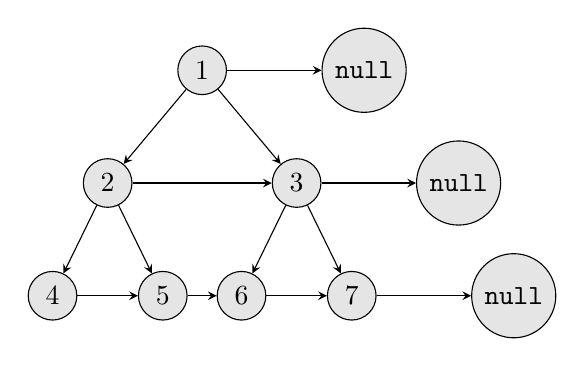
\begin{tikzpicture}
[mynode/.style={draw,circle,minimum size=5mm, fill=gray!20!}]
\node(){};
\node[mynode](1) {1};
\node[mynode](r1) [right = 12mm of 1] {\texttt{null}};
\node[mynode](2) [below = 8mm of 1, xshift=-12mm] {2};
\node[mynode](3) [below = 8mm of 1, xshift=12mm] {3};
\node[mynode](r2) [right = 12mm of 3] {\texttt{null}};
\node[mynode](4) [below = 8mm of 2, xshift=-7mm] {4};
\node[mynode](5) [below = 8mm of 2, xshift=7mm] {5};
\node[mynode](6) [below = 8mm of 3, xshift=-7mm] {6};
\node[mynode](7) [below = 8mm of 3, xshift=7mm] {7};
\node[mynode](r3) [right = 12mm of 7] {\texttt{null}};
\draw[>=stealth,->] (1) -- (2);
\draw[>=stealth,->] (1) -- (3);
\draw[>=stealth,->] (2) -- (4);
\draw[>=stealth,->] (2) -- (5);
\draw[>=stealth,->] (3) -- (6);
\draw[>=stealth,->] (3) -- (7);
\draw[>=stealth,->] (1) -- (r1);
\draw[>=stealth,->] (3) -- (r2);
\draw[>=stealth,->] (7) -- (r3);
\draw[>=stealth,->] (2) -- (3);
\draw[>=stealth,->] (4) -- (5);
\draw[>=stealth,->] (5) -- (6);
\draw[>=stealth,->] (6) -- (7);
\end{tikzpicture}
\end{figure}
\end{flushleft}
\subsection{Analysis}
由于要求只能用$O(1)$的存储空间,因此需要有效利用$\texttt{next}$指针来联系左右节点。由于是否存在左右节点只能由父节点来判断,因此需要根据parent node的next来判断是否旁边还有node。由于已经明确了是完全二叉树,因此每个节点除了根节点之外都会有兄弟节点。而循环只需要走到叶子节点上层即可。

\setcounter{lstlisting}{0}
\begin{lstlisting}[style=customc, caption={Iterative}]
Node* connect( Node* root )
{
    if( !root )
    {
        return root;
    }
    auto node = root;
    while( node->left )
    {
        auto t = node;
        while( t )
        {
            //connect left and right
            t->left->next = t->right;
            if( t->next )
            {
                //connect right to right sibling's left
                t->right->next = t->next->left;
            }
            //move to its sibling
            t = t->next;
        }
        //move to its child node
        node = node->left;
    }
    return root;
}
\end{lstlisting}

%\section{117 --- Populating Next Right Pointers in Each Node II}
Given a binary tree $T$
\begin{lstlisting}
struct TreeLinkNode {
  TreeLinkNode *left;
  TreeLinkNode *right;
  TreeLinkNode *next;
}
\end{lstlisting}
\par
Populate each next pointer to point to its next right node. If there is no next right node, the next pointer should be set to \texttt{null}.
\par
Initially, all next pointers are set to \texttt{null}.
\paragraph{Note:}
\begin{itemize}
    \item You may only use constant extra space.
    \item Recursive approach is fine, implicit stack space does not count as extra space for this problem.
\end{itemize}
\paragraph{Example:}
\begin{flushleft}
\textbf{Input}
\begin{figure}[H]
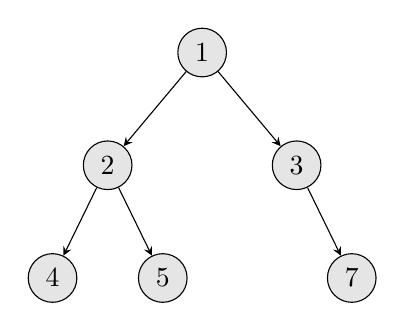
\begin{tikzpicture}
[mynode/.style={draw,circle,minimum size=5mm, fill=gray!20!}]
\node(){};
\node[mynode](1) {1};
\node[mynode](2) [below = 8mm of 1, xshift=-12mm] {2};
\node[mynode](3) [below = 8mm of 1, xshift=12mm] {3};
\node[mynode](4) [below = 8mm of 2, xshift=-7mm] {4};
\node[mynode](5) [below = 8mm of 2, xshift=7mm] {5};
\node[mynode](7) [below = 8mm of 3, xshift=7mm] {7};
\draw[>=stealth,->] (1) -- (2);
\draw[>=stealth,->] (1) -- (3);
\draw[>=stealth,->] (2) -- (4);
\draw[>=stealth,->] (2) -- (5);
\draw[>=stealth,->] (3) -- (7);
\end{tikzpicture}
\end{figure}
\textbf{Output}:
\begin{figure}[H]
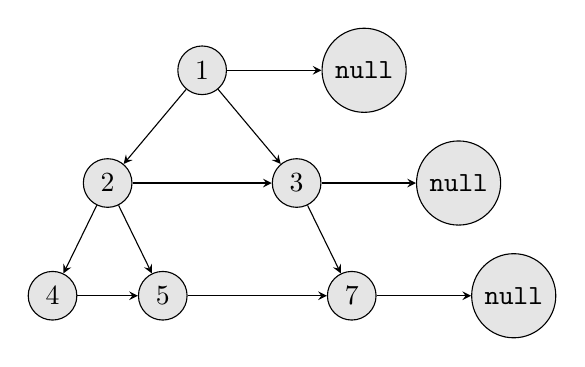
\begin{tikzpicture}
[mynode/.style={draw,circle,minimum size=5mm, fill=gray!20!}]
\node(){};
\node[mynode](1) {1};
\node[mynode](r1) [right = 12mm of 1] {\texttt{null}};
\node[mynode](2) [below = 8mm of 1, xshift=-12mm] {2};
\node[mynode](3) [below = 8mm of 1, xshift=12mm] {3};
\node[mynode](r2) [right = 12mm of 3] {\texttt{null}};
\node[mynode](4) [below = 8mm of 2, xshift=-7mm] {4};
\node[mynode](5) [below = 8mm of 2, xshift=7mm] {5};
\node[mynode](7) [below = 8mm of 3, xshift=7mm] {7};
\node[mynode](r3) [right = 12mm of 7] {\texttt{null}};
\draw[>=stealth,->] (1) -- (2);
\draw[>=stealth,->] (1) -- (3);
\draw[>=stealth,->] (2) -- (4);
\draw[>=stealth,->] (2) -- (5);
\draw[>=stealth,->] (3) -- (7);
\draw[>=stealth,->] (1) -- (r1);
\draw[>=stealth,->] (3) -- (r2);
\draw[>=stealth,->] (7) -- (r3);
\draw[>=stealth,->] (2) -- (3);
\draw[>=stealth,->] (4) -- (5);
\draw[>=stealth,->] (5) -- (7);
\end{tikzpicture}
\end{figure}
\end{flushleft}
\subsection{Level Traversing}
\begin{CJK*}{UTF8}{gbsn}
虽然题目要求中可能不是完全二叉树,但是基本思路仍然是用指针分别指向当前节点以及下层节点的首节点以及下层节点的当前节点。保留下层节点的首节点是当遍历完当前level的时候,能够move到下一层。
\end{CJK*}
\setcounter{algorithm}{0}
\begin{algorithm}[H]
\caption{Iterative Approach}
\begin{algorithmic}[1]
\Procedure{Connect}{$T$}
\If{$T=\texttt{null}$}
\State \Return
\EndIf
\State $x:=T$ \Comment Current node of current level
\State $y:=\texttt{null}$ \Comment Current node of next level
\State $z:=\texttt{null}$ \Comment The first node of next level
\While{$x\neq \texttt{null}$}
\State $t:=x$
\While{$t\neq \texttt{null}$} \label{117while1} 
\If{$\texttt{Left}(t) \neq \texttt{null}$}
\If{$y\neq \texttt{null}$}
\State $\texttt{Next}(y)\gets \texttt{Left}(t)$ \Comment Link sibling's left node
\Else \Comment $t$'s left node is the first node
\State $z\gets \texttt{Left}(t)$
\EndIf
\State $y\gets \texttt{Left}(t)$ \Comment Move $y$ to the next node in next level
\EndIf
\If{$\texttt{Right}(t) \neq \texttt{null}$}
\If{$y\neq \texttt{null}$}
\State $\texttt{Next}(y)\gets \texttt{Right}(t)$ \Comment Link sibling's left node
\Else \Comment $t$'s right node is the first node
\State $z\gets \texttt{Right}(t)$
\EndIf
\State $y\gets \texttt{Right}(t)$ \Comment Move $y$ to the next node in next level
\EndIf
\State $t\gets \texttt{Next}(t)$ \Comment Update $t$ to next sibling node
\algstore{117algo}
\end{algorithmic}
\end{algorithm}
\begin{algorithm}[H]
\begin{algorithmic}[1]
\algrestore{117algo}
\EndWhile \Comment End [\ref{117while1}]
\State $x\gets z$ \Comment Move $x$ to next level
\State $z\gets \texttt{null}$ \Comment Reset $z$ as empty
\State $y\gets \texttt{null}$ \Comment Reset $y$ as empty
\EndWhile
\EndProcedure
\end{algorithmic}
\end{algorithm}
%\section{118 --- Pascal's Triangle}
Given a non-negative integer \fcj{numRows}, generate the first \fcj{numRows} of Pascal's triangle.

In Pascal's triangle, each number is the sum of the two numbers directly above it.
\paragraph{Example:}
\begin{flushleft}
\textbf{Input}: 5
\\
\textbf{Output}:

\fcj{[[1], [1,1], [1,2,1], [1,3,3,1], [1,4,6,4,1]]}
\end{flushleft}
\subsection{Analysis}

每一层的首个和结尾一个数字都是1,从第三层开始,中间的每个数字都是上一行的左右两个数字之和

\setcounter{lstlisting}{0}
\begin{lstlisting}[style=customc, caption={DP}]
vector<vector<int>> generate( int numRows )
{
    vector<vector<int>> ans;
    if( numRows == 0 )
    {
        return ans;
    }
    ans.emplace_back( vector<int> {1} );
    for( int r = 2; r <= numRows; ++r )
    {
        vector<int> cur( r, 1 );
        //the head and tail are 1
        //fill from index = 1 to r-2
        for( int i = 1; i < r - 1; ++i )
        {
            cur[i] = ans.back()[i - 1] + ans.back()[i];
        }
        ans.emplace_back( vector<int> {} );
        ans.back().swap( cur );
    }
    return ans;
}
\end{lstlisting}

%\section{119 --- Pascal's Triangle II}
Given a non-negative index $k$ where $k \leq 33$, return the $k$th index row of the Pascal's triangle.
\par
Note that the row index starts from 0.
\par
In Pascal's triangle, each number is the sum of the two numbers directly above it.
\paragraph{Example:}
\begin{flushleft}
\textbf{Input}: 3
\\
Output: $[1,\;3,\;3,\;1]$
\end{flushleft}
\paragraph{Follow up:}
\begin{flushleft}
Could you optimize your algorithm to use only $O(k)$ extra space?
\end{flushleft}
\subsection{Analysis}
\begin{CJK*}{UTF8}{gbsn}
如果只能用$O(k)$的存储空间,那么为了重复利用这个存储空间,必须想办法如何既能得到新一层的值而同时能够保留需要用的上一层的值,办法就是从第二层开始,每一层都是从最后一个元素往前更新,这样,当前元素更新后,不影响上一层其左边元素的值。比如$k=3$,那么数组的更新顺序结果如下
\begin{itemize}
\item $k=0$: $[1,0,0,0]$
\item $k=1$: $[1,1,0,0]$
\item $k=2$: $[1,2,1,0]$
\item $k=3$: $[1,3,3,1]$
\end{itemize}
\end{CJK*}
\setcounter{algorithm}{0}
\begin{algorithm}[H]
\caption{Update From End To Front}
\begin{algorithmic}[1]
\Procedure{GetRow}{$k$}
\State $A$ as $A[0]:=1,\;A[1]=\ldots=A[k]=0$
\For{$x=1 \to k$}
\For{$y=k \to 1$}
\State $A[y]\gets A[y] + A[y-1]$ \Comment Update $A[y]$ but $A[y-1]$ is not affected
\EndFor
\EndFor
\State \Return $A$
\EndProcedure
\end{algorithmic}
\end{algorithm}

%\section{120 --- Triangle}
Given a triangle $T$, find the minimum path sum from top to bottom. Each step you may move to adjacent numbers on the row below.
\paragraph{Example}
\begin{flushleft}
\textbf{Input}:
\begin{table}[H]
\begin{tabular}{llll}
2 &   &   &   \\
3 & 4 &   &   \\
6 & 5 & 7 &   \\
4 & 1 & 8 & 3
\end{tabular}
\end{table}
\textbf{Output}: 11
\\
\textbf{Explanation}:
The minimum path sum from top to bottom is 11 (i.e., $2 + 3 + 5 + 1 = 11$).
\end{flushleft}
\paragraph{Note:}
\begin{itemize}
\item Bonus point if you are able to do this using only $O(n)$ extra space, where $n$ is the total number of rows in the triangle.
\end{itemize}
\subsection{Dynamic Programming}
\begin{CJK*}{UTF8}{gbsn}
表面上看,这个三角形看起来像一个树状结构,这很自然让我们想到用树的遍历算法比如DFS。但是,如果仔细观察就会发现,其实相邻的nodes构成了一个选择分支。也就是说,存在\textbf{overlapping subproblems}。而且,如果$x, y$是$k$的adjacent nodes,一旦找到了minimum path starting from $x$ and $y$,那么minimum path starting from $k$也就找到了,这就构成了一个\textbf{optimal substructure}。因此,Dynamic Programming是最佳的solution。
\end{CJK*}
\par
\begin{CJK*}{UTF8}{gbsn}
如果采用\textbf{Top--Down}的方式,从最顶层的node出发,递归寻找每个node的minium path sum。每次计算出一个path sum,就存放在一个数组中。下一次需要计算同一个node的minimum path sum时,只需要直接从存放的数组中获得。但是这个数组的大小至少要与输入的三角形数组的大小相等,而这需要$O(N^2)$存储空间。虽然也能通过某些trick优化这个存储空间,但是这在recursive方法中很难直接想到。
\end{CJK*}
\par
\begin{CJK*}{UTF8}{gbsn}
反之,如果采用\textbf{Bottom--Up}的方式,优化存储空间就很直接了。首先从最底层的node出发,最开始每个node的minimum path sum就是node本身的值。接着,在$k$th row的$i$th node的minimum path sum就是这个节点的两个children的minimum path sum中的最小值加上这个节点的值。即:
\end{CJK*}
\[
F(k,i)=\min(F(k+1, i), F(k+1, i+1)) + T[k][i]
\]
\begin{CJK*}{UTF8}{gbsn}
接下来就是如何优化存储空间,我们需要将$F$修改成1D array,然后iteratively逐步更新$F$,即对于$k$th level
\end{CJK*}
\[
F[i] = \min(F[i], F[i+1]) + T[k][i];
\]
\begin{CJK*}{UTF8}{gbsn}
最后$F[0]$就是最终的结果。
\end{CJK*}
\setcounter{algorithm}{0}
\begin{algorithm}[H]
\caption{Dynamic Programming}
\begin{algorithmic}[1]
\Procedure{MinimumTotal}{$T,\;L_T$}
\State $F:=T[L_T-1]$ \Comment $F$ is initialized as the final element in $T$
\For{$l:=L_T-2 \to 0$}
\For{$i:=0 \to l$}
\State $F[i]\gets \min(F[i], F[i+1]) + T[l][i]$
\EndFor
\EndFor
\State \Return $F[0]$
\EndProcedure
\end{algorithmic}
\end{algorithm}
%\section{121 --- Best Time to Buy and Sell Stock}
Say you have an array $P$ for which the $i$th element is the price of a given stock on day $i$.
\par
If you were only permitted to complete at most one transaction (i.e., buy one and sell one share of the stock), design an algorithm to find the maximum profit.
\par
Note that you cannot sell a stock before you buy one.
\paragraph{Example 1:}
\begin{flushleft}
\textbf{Input}: $[7,\;1,\;5,\;3,\;6,\;4]$
\\
\textbf{Output}: 5
\\
\textbf{Explanation}
\\
Buy on day 2 (price = 1) and sell on day 5 (price = 6), profit = $6-1 = 5$. Not $7-1 = 6$, as selling price needs to be larger than buying price.
\end{flushleft}
\paragraph{Example 2:}
\begin{flushleft}
\textbf{Input}: $[7,\;6,\;4,\;3,\;1]$
\\
\textbf{Output}: 0
\\
\textbf{Explanation}: In this case, no transaction is done, i.e. max profit is 0.
\end{flushleft}
\subsection{Minimum Price}
\begin{CJK*}{UTF8}{gbsn}
遍历数组,用$x$是代表目前遇到的price中的最小值,那么当前的price与$x$的差值即为可能的最大profit
\end{CJK*}
\setcounter{algorithm}{0}
\begin{algorithm}[H]
\caption{Minimum Price So Far}
\begin{algorithmic}[1]
\Procedure{MaxProfit}{$P,\;L_P$}
\If{$L_P=0$}
\State \Return 0
\EndIf
\State $x:=P[0]$ \Comment The minimum price so far
\State $\texttt{ans}:=0$ \Comment The maximum profit
\For{$i:=1 \to L_P-1$}
\State $x\gets \min(x, P[i])$ \Comment Update minimum price so far
\State $\texttt{ans}\gets \max(\texttt{ans}, P[i] - x)$ \Comment Update maximum profit
\algstore{121algo}
\end{algorithmic}
\end{algorithm}
\begin{algorithm}[H]
\begin{algorithmic}[1]
\algrestore{121algo}
\EndFor
\State \Return \texttt{ans}
\EndProcedure
\end{algorithmic}
\end{algorithm}
\subsection{Kadane Algorithm}
The logic to solve this problem is same as \textit{maximum subarray problem} using \textbf{Kadane Algorithm}. If the question is changed slightly by giving the difference array of prices, For example: for a given array $[1,\;7,\;4,\;11]$, the problem could give the difference as $[0,\;6,\;-3,\;7]$. Here, the logic is to calculate the difference $( D = D + P[i] - P[i-1])$ of the original array, and find a contiguous subarray giving maximum profit. If the difference falls below 0, reset it to zero.
\begin{algorithm}[H]
\caption{Kadane Algorithm}
\begin{algorithmic}[1]
\Procedure{MaxProfit}{$P,\;L_P$}
\If{$L_P=0$}
\State \Return 0
\EndIf
\State $x:=0$
\State $\texttt{ans}:=0$
\For{$i:=1\to L_P-1$}
\State $x\gets \max(0, x + P[i] - P[i-1])$
\State $\texttt{ans}\gets \max(\texttt{ans},x)$
\EndFor
\State \Return \texttt{ans}
\EndProcedure
\end{algorithmic}
\end{algorithm}

%\section{122 --- Best Time to Buy and Sell Stock II}
Say you have an array $P$ for which the $i$th element is the price of a given stock on day $i$.

Design an algorithm to find the maximum profit. You may complete as many transactions as you like (i.e., buy one and sell one share of the stock multiple times).

Note: You may not engage in multiple transactions at the same time (i.e., you must sell the stock before you buy again).
\paragraph{Example 1:}
\begin{flushleft}
\textbf{Input}: $[7,\;1,\;5,\;3,\;6,\;4]$
\\
\textbf{Output}: 7
\\
\textbf{Explanation}
\\
Buy on day 2 (price = 1) and sell on day 3 (price = 5), profit $= 5-1 = 4$. Then buy on day 4 (price = 3) and sell on day 5 (price = 6), profit $= 6-3 = 3$.
\end{flushleft}
\paragraph{Example 2:}
\begin{flushleft}
\textbf{Input}: $[1,\;2,\;3,\;4,\;5]$
\\
\textbf{Output}: 4
\\
\textbf{Explanation}
\\
Buy on day 1 (price = 1) and sell on day 5 (price = 5), profit $= 5-1 = 4$. Note that you cannot buy on day 1, buy on day 2 and sell them later, as you are engaging multiple transactions at the same time. You must sell before buying again.
\end{flushleft}
\paragraph{Example 3:}
\begin{flushleft}
\textbf{Input}: $[7,\;6,\;4,\;3,\;1]$
\\
\textbf{Output}: 0
\\
\textbf{Explanation}
\\
In this case, no transaction is done, i.e. max profit $= 0$.
\end{flushleft}
\subsection{Simple One Pass}
这里条件放宽了,可以无限次买入和卖出。因此只需要从第二天开始,如果当前价格比之前价格高,则把差值加入利润中,因为我们可以昨天买入,今日卖出,若明日价更高的话,还可以今日买入,明日再抛出。以此类推,遍历完整个数组后即可求得最大利润

%\section{123 --- Best Time to Buy and Sell Stock III}
Say you have an array $P$ for which the $i$th element is the price of a given stock on day $i$.
\par
Design an algorithm to find the maximum profit. You may complete at most \textbf{two} transactions.
\par
Note: You may not engage in multiple transactions at the same time (i.e., you must sell the stock before you buy again).
\paragraph{Example 1:}
\begin{flushleft}
\textbf{Input}: $[3,\;3,\;5,\;0,\;0,\;3,\;1,\;4]$
\\
\textbf{Output}: 6
\\
\textbf{Explanation}: Buy on day 4 (price = 0) and sell on day 6 (price = 3), profit $= 3-0 = 3$. Then buy on day 7 (price = 1) and sell on day 8 (price = 4), profit $= 4-1 = 3$.
\end{flushleft}
\paragraph{Example 2:}
\begin{flushleft}
\textbf{Input}: $[1,\;2,\;3,\;4,\;5]$
\\
\textbf{Output}: 4
\\
\textbf{Explanation}: Buy on day 1 (price = 1) and sell on day 5 (price = 5), profit $= 5-1 = 4$.Note that you cannot buy on day 1, buy on day 2 and sell them later, as you are engaging multiple transactions at the same time. You must sell before buying again.
\end{flushleft}
\paragraph{Example 3:}
\begin{flushleft}
\textbf{Input}: $[7,\;6,\;4,\;3,\;1]$
\\
\textbf{Output}: 0
\\
\textbf{Explanation}: In this case, no transaction is done, i.e. max profit $= 0$.
\end{flushleft}
\subsection{General Approach}
解决类似的问题有一个一般性的方法可以处理。基本思想是创建两个table $H$ and $U$。其中
\begin{itemize}
\item $H[i][j]$表示当持有股票时,从0到$i$th天最多发生$j$次transaction所能获得的最大profit。而
\item $U[i][j]$表示当不持有股票时,从0到$i$th天最多发生$j$次transaction所能获得的最大profit。
\end{itemize}
对应的递推公式为
\begin{align*}
H[i][j] &= \max(U[i-1][j]-P[i], H[i-1][j]) \\
U[i][j] &= \max(H[i-1][j-1] + P[i], U[i-1][j])
\end{align*}
公式1的意义表示,如果在第$i$天手头持有股票,那么要么是第$i$天买入股票或者在第$i$天前已经买入了股票,
\begin{enumerate}
\item 如果在第$i$天买入股票,由于只是买入,并没有卖出,因此不算一个transaction,而这时候购买股票需要花费$P[i]$,而第$i-1$天手头没有股票,因此相应的利润就是$U[i-1][j] - P[i]$。
\item 如果第$i$天没有买入股票,这时候第$i-1$天肯定持有股票了,因此这时候的利润就和第$i-1$天持有股票的利润相等,即$H[i-1][j]$
\end{enumerate}
公式2也是基于类似的理由,唯一不同的是,如果在$i$天卖出股票,由于手头持有股票才能卖,所以这算一个transaction,因此在$i-1$天的利润就是$H[i-1][j-1]$。

最后就是初始化时,
\begin{itemize}
\item $U[0][i]=U[i][0]:=0$,$U[0][i]$即在第0天手头没有股票的利润很显然是0,$U[i][0]$即没有发生transaction时手头没有股票的利润,很显然也是0。
\item 对于$H[0][0]$,即在第0天买入股票并持有,其利润即为$-P[0]$,对于$i>0$,$H[0][i]$即在第0天买入股票并持有并发生$i>1$次transaction,因为只有一天而且是持有股票,这个利润必须就是$-P[0]$。而$H[i][0]$即状态变成手头持有股票从第0天到第$i$天发生0次transaction所能产生的最大利润,由于是第$i$天状态仍然是持有股票,并且是0交易,所以要么在$i-1$天前已经是持有股票的状态,要么只是在$i$天才持有股票,因此$H[i][0]=\max(H[i-1][0], -P[i])$。
\end{itemize}

\setcounter{lstlisting}{0}
\begin{lstlisting}[style=customc, caption={DP}]
int maxProfit( vector<int>& prices )
{
    if( prices.empty() )
    {
        return 0;
    }
    //the maximum profit when hold a stock at day i with transaction j
    vector<array<int, 3>> stock( prices.size(), {0, 0, 0} );
    //the maximum profit when not holding a stock at day i with transaction j
    vector<array<int, 3>> cash( prices.size(), {0, 0, 0} );
    stock[0][0] = -prices[0];
    for( size_t i = 1; i < prices.size(); ++i )
    {
        //at day i without any transaction
        //we either hold stock at day (i - 1)
        //or we bought a stock at day (i)
        //only buy without sell is not one transaction
        stock[i][0] = ( max )( stock[i - 1][0], -prices[i] );
    }
    stock[0][1] = -prices[0];
    stock[0][2] = -prices[0];
    for( size_t i = 1; i < prices.size(); ++i )
    {
        //stock[i][k]: either we have stock at day (i-1) with k transaction
        //or we bought a stock at day (i-1) with k transaction
        //notice: only buy without sell is not one transaction
        stock[i][1] = ( max )( cash[i - 1][1] - prices[i], stock[i - 1][1] );
        stock[i][2] = ( max )( cash[i - 1][2] - prices[i], stock[i - 1][2] );
        //cash[i][k]: either we have stock at day (i-1) with (k-1) transactions
        //and sell it on day i
        //or we doesn't have stock at day (i-1) with (k) transactions
        cash[i][1] = ( max )( stock[i - 1][0] + prices[i], cash[i - 1][1] );
        cash[i][2] = ( max )( stock[i - 1][1] + prices[i], cash[i - 1][2] );
    }
    //we can do maximum 2 transactions
    return ( max )( stock.back()[2], cash.back()[2] );
}
\end{lstlisting}



%\section{124 --- Binary Tree Maximum Path Sum}
Given a non-empty binary tree $T$, find the maximum path sum.
\par
For this problem, a path is defined as any sequence of nodes from some starting node to any node in the tree along the parent-child connections. The path must contain \textbf{at least one node} and does not need to go through the root.
\paragraph{Example 1:}
\begin{flushleft}
\textbf{Input}:
\begin{figure}[H]
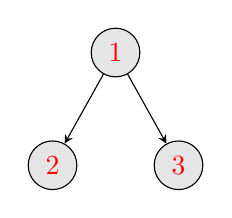
\begin{tikzpicture}
[mynode/.style={draw,circle,minimum size=5mm, fill=gray!20!}]
\node(){};
\node[mynode](1) {\textcolor{red}{1}};
\node[mynode](2)[below=8mm of 1, xshift=-8mm] {\textcolor{red}{2}};
\node[mynode](3)[below=8mm of 1, xshift=8mm] {\textcolor{red}{3}};
\draw[>=stealth,->] (1) -- (2);
\draw[>=stealth,->] (1) -- (3);
\end{tikzpicture}
\end{figure}
\textbf{Output}: 6
\end{flushleft}
\paragraph{Example 2:}
\begin{flushleft}
\textbf{Input}:
\begin{figure}[H]
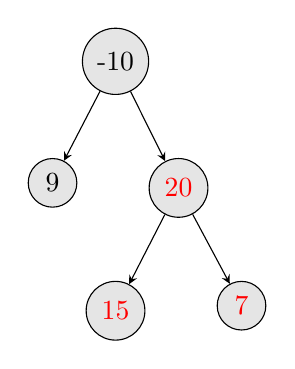
\begin{tikzpicture}
[mynode/.style={draw,circle,minimum size=5mm, fill=gray!20!}]
\node(){};
\node[mynode](1) {-10};
\node[mynode](2)[below=8mm of 1, xshift=-8mm] {9};
\node[mynode](3)[below=8mm of 1, xshift=8mm] {\textcolor{red}{20}};
\node[mynode](4)[below=8mm of 3, xshift=-8mm] {\textcolor{red}{15}};
\node[mynode](5)[below=8mm of 3, xshift=8mm] {\textcolor{red}{7}};
\draw[>=stealth,->] (1) -- (2);
\draw[>=stealth,->] (1) -- (3);
\draw[>=stealth,->] (3) -- (4);
\draw[>=stealth,->] (3) -- (5);
\end{tikzpicture}
\end{figure}
\textbf{Output}: 42
\end{flushleft}
\subsection{DFS}
\begin{figure}[H]
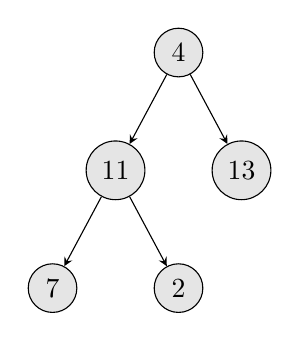
\begin{tikzpicture}
[mynode/.style={draw,circle,minimum size=5mm, fill=gray!20!}]
\node(){};
\node[mynode](1) {4};
\node[mynode](2)[below=8mm of 1, xshift=-8mm] {11};
\node[mynode](3)[below=8mm of 1, xshift=8mm] {13};
\node[mynode](4)[below=8mm of 2, xshift=-8mm] {7};
\node[mynode](5)[below=8mm of 2, xshift=8mm] {2};
\draw[>=stealth,->] (1) -- (2);
\draw[>=stealth,->] (1) -- (3);
\draw[>=stealth,->] (2) -- (4);
\draw[>=stealth,->] (2) -- (5);
\end{tikzpicture}
\end{figure}
\begin{CJK*}{UTF8}{gbsn}
以图中所示的树为例子,很容易就能找到最长路径为$7\to11\to4\to13$,由于树的递归解法一般都是递归到叶节点,然后开始处理并回溯到根节点。假设此时已经递归到结点7了,那么其没有左右子节点,所以以结点7为根结点的子树最大路径和就是7。然后回溯到结点11。而以结点11为根结点的子树的最大路径和为$7+11+2=20$。但是当回溯到结点4的时候,对于结点11来说,就不能同时取两条路径了,只能取左路径,或者是右路径,所以当根结点是4的时候,那么结点11只能取其左子结点7,因为7大于2。所以,对于每个结点来说,需要比较经过其left child的path sum以及经过right child的path sum,看这两个值哪个大。因此递归函数返回值就可以定义为以当前结点为根结点,到叶子节点的最大路径之和,然后全局路径最大值放在函数的输入参数中。
\end{CJK*}
\par
\begin{CJK*}{UTF8}{gbsn}
在递归函数中,如果当前结点不存在,那么直接返回0。否则就分别对其左右子节点调用递归函数,由于path sum有可能为负数,加上负数只会让结果更小,因此需要和零比较,取较大的那个。然后更新全局最大值,而这个值就是以left child为起点的最大path sum加上以right child为起点的最大path sum,再加上当前结点值,这样就组成了一条完整的路径。而返回值是取左右两个path sum中的较大值加上当前结点值,因为返回值的定义是以当前结点为起点的path sum,所以只能取左右两个path sum中的一个。
\end{CJK*}
\setcounter{algorithm}{0}
\begin{algorithm}[H]
\caption{DFS}
\begin{algorithmic}[1]
\Procedure{MaxPathSum}{$T$}
\State $\texttt{ans}:=-\infty$
\State $\texttt{DFS}(T,\;\texttt{ans})$ \Comment Call helper function \texttt{DFS}
\State \Return \texttt{ans}
\EndProcedure
\end{algorithmic}
\end{algorithm}
\begin{CJK*}{UTF8}{gbsn}
Function \texttt{DFS}递归遍历二叉树$T$,并更新最大的path sum $S$。
\end{CJK*}
\begin{algorithm}[H]
\caption{Helper Function}
\begin{algorithmic}[1]
\Function{DFS}{$T,\;S$}
\If{$T=\texttt{null}$}
\State \Return 0
\EndIf
\State $x:=\texttt{DFS}(\texttt{Left}(T),\;S)$ \Comment Recursive on left subtree
\State $y:=\texttt{DFS}(\texttt{Right}(T),\;S)$ \Comment Recursive on right subtree
\State $x\gets \max(0, x)$ \Comment Negative value is neglected
\State $y\gets \max(0, y)$ \Comment Negative value is neglected
\State $S\gets \max(S, x+y+\texttt{Value}(T))$ \Comment Update max path sum so far
\State \Return $\max(x,y) + \texttt{Value}(T)$ \Comment Returns the max path sum starting with $T$
\algstore{124algo}
\end{algorithmic}
\end{algorithm}
\begin{algorithm}[H]
\begin{algorithmic}[1]
\algrestore{124algo}
\EndFunction
\end{algorithmic}
\end{algorithm}
%\section{125 --- Valid Palindrome}
Given a string $S$, determine if it is a palindrome, considering only alphanumeric characters and ignoring cases.
\par
Note: For the purpose of this problem, we define empty string as valid palindrome.
\paragraph{Example 1:}
\begin{flushleft}
\textbf{Input}: $S=\text{A man, a plan, a canal: Panama}$
\\
\textbf{Output}: \textit{true}
\end{flushleft}
\paragraph{Example 2:}
\begin{flushleft}
\textbf{Input}: $S=\text{race a car}$
\\
\textbf{Output}: \textit{false}
\end{flushleft}
\subsection{Analysis}
\begin{CJK*}{UTF8}{gbsn}
很简单的题目,用$\alpha$,$\beta$分别代表指向字符串左边和右边的两个index, 分别从字符的开头和结尾处开始遍历整个字符串,如果遇到非字母数字的字符就跳过,继续往下找,直到找到下一个字母数字或者结束遍历,如果遇到小写字母,就将其转为大写。等左右指针都找到字母数字时,比较这两个字符,若相等,则继续比较下面两个分别找到的字母数字,若不相等,直接返回\textit{false}
\end{CJK*}
%\section{126 --- Word Ladder II}
Given two words (\fcj{beginWord} and \fcj{endWord}), and a dictionary's word list, find all shortest transformation sequence(s) from \fcj{beginWord} to \fcj{endWord}, such that:
\begin{itemize}
\item Only one letter can be changed at a time
\item Each transformed word must exist in the word list. Note that \fcj{beginWord} is not a transformed word.
\end{itemize}
\paragraph{Note:}
\begin{itemize}
\item Return an empty list if there is no such transformation sequence.
\item All words have the same length.
\item All words contain only lowercase alphabetic characters.
\item You may assume no duplicates in the word list.
\item You may assume \fcj{beginWord} and \fcj{endWord} are non-empty and are not the same.
\end{itemize}
\paragraph{Example 1:}
\begin{flushleft}
\textbf{Input}: 

\fcj{beginWord = "hit"}

\fcj{endWord = "cog"}

\fcj{wordList = ["hot","dot","dog","lot","log","cog"]}

\textbf{Output}:

\fcj{["hit","hot","dot","dog","cog"]}

\fcj{["hit","hot","lot","log","cog"]}

\end{flushleft}

\paragraph{Example 2:}
\begin{flushleft}
\textbf{Input}: 

\fcj{beginWord = "hit"}

\fcj{endWord = "cog"}

\fcj{wordList = ["hot","dot","dog","lot","log"]}

\textbf{Output}: 

\fcj{[]}


\textbf{Explanation}: The endWord \fcj{"cog"} is not in wordList, therefore no possible transformation.
\end{flushleft}
\subsection{Bidirectional BFS}
假设同时从$\alpha$和$\beta$出发进行宽度优先扩展,如果可以在两个树的某一层找到相同的word,这时候就能确定最短距离了,即最早产生相同word的层数。以给出的例子说明,从begin word \textbf{hot}出发,其扩展出的BFS tree前三层如下所示
\begin{figure}[H]
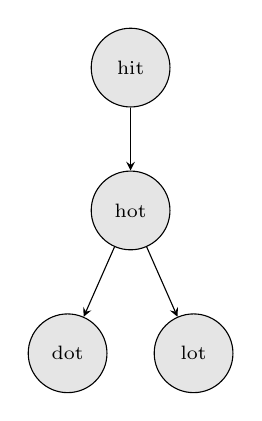
\begin{tikzpicture}
[mynode/.style={draw,circle,minimum size=10mm, fill=gray!20!}]
\node(){};
\node[mynode](1) {\scriptsize hit};
\node[mynode](2)[below=8mm of 1] {\scriptsize hot};
\node[mynode](3)[below=8mm of 2, xshift=-8mm] {\scriptsize dot};
\node[mynode](4)[below=8mm of 2, xshift=8mm] {\scriptsize lot};
\draw[>=stealth,->] (1) -- (2);
\draw[>=stealth,->] (2) -- (3);
\draw[>=stealth,->] (2) -- (4);
\end{tikzpicture}
\end{figure}
而从end word \textbf{cog}出发,其扩展出的BFS tree 前三层如下所示。
\begin{figure}[H]
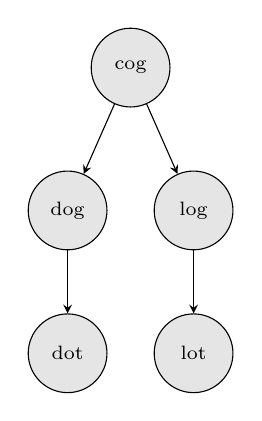
\begin{tikzpicture}
[mynode/.style={draw,circle,minimum size=10mm, fill=gray!20!}]
\node(){};
\node[mynode](1) {\scriptsize cog};
\node[mynode](2)[below=8mm of 1, xshift=-8mm] {\scriptsize dog};
\node[mynode](3)[below=8mm of 1, xshift=8mm] {\scriptsize log};
\node[mynode](4)[below=8mm of 2] {\scriptsize dot};
\node[mynode](5)[below=8mm of 3] {\scriptsize lot};
\draw[>=stealth,->] (1) -- (2);
\draw[>=stealth,->] (1) -- (3);
\draw[>=stealth,->] (2) -- (4);
\draw[>=stealth,->] (3) -- (5);
\end{tikzpicture}
\end{figure}
注意在上图中虽然\textbf{dog}也能transform到\textbf{log},但是由于\textbf{log}也同样能从\textit{cog}中得到,而我们是为了得到最短的路径,所以\textbf{log}选择从\textit{cog}变换得到。同理,\textbf{dog}也由\textit{cog}转换得到,而不是从\textbf{log}。这样在具体实现时,我们需要将已经transform得到的word从保存的可transform的word list $A$中删除。这时候可以看到两个word扩展出的树的第三层有相同的word,因此这一层就是最短的路径。

在实现时,用一个hash map记录每个word所transform出的单词,可能是一个也可能是多个,因此这个hash map的value就是一个array。由于我们是从两个方向同时进行DFS,因此每次选择DFS的开始层时,总是选择node最少的层开始,另外就是注意由于是两个方向,而hash map所记录的转换关系是单向的,即是从$\alpha$到$\beta$,所以如果当前处理的方向是从$\beta$到$\alpha$,那么在更新hash map时,要把tranform出的word作为key,而作为transform源头的word放入key对应的array中。

有了最短路径后,我们就得到了每个word及其transform出的word,接下来就可以用递归即DFS的方式构建出path了。
\setcounter{algorithm}{0}
\begin{algorithm}[H]
\caption{Bidirectional BFS Search + DFS Path Building}
\begin{algorithmic}[1]
\Procedure{FindLadders}{$\alpha,\;\beta,\;A$}
\If{$\beta\notin A$} \Comment The end word is not in the word list
\State \Return $\emptyset$ \Comment Cannot reach end word through $A$
\EndIf
\State $A\gets A\setminus \beta$ \Comment Remove end word from $A$
\algstore{126algo}
\end{algorithmic}
\end{algorithm}
\begin{algorithm}[H]
\begin{algorithmic}[1]
\algrestore{126algo}
\State $x:=\emptyset,\ y:=\emptyset$ \Comment Two hash sets to simulate BFS tree
\State $x\gets x + \alpha$ \Comment The forward BFS tree root
\State $y\gets y + \alpha$ \Comment The backward BFS tree root
\State $C:=\emptyset$ \Comment The hash map contains the words and transformed words from each word
\State $b:=\texttt{false}$ \Comment Indicate if the two trees have same words in their respective current level
\State $d:=0$ \Comment Indicate the type of current tree (0 is forward tree and 1 is backward tree)
\While{$x\neq \emptyset$ \textbf{and} $y\neq\emptyset$ and $b:=\texttt{false}$}
\For{$w \in x$}
\State $A\gets A\setminus w$ \Comment Remove transformed words in $x$ from $A$ to avoid repeating search
\EndFor
\For{$w \in y$}
\State $A\gets A\setminus w$ \Comment Remove transformed words in $y$ from $A$ to avoid repeating search
\EndFor
\If{$|x| \leq |y|$} \Comment $x$ has fewer or equal nodes than $y$
\State $\texttt{Process}(x, y, C, A, b, \texttt{forward})$ \Comment Forward direction
\Else 
\State $\texttt{Process}(y, x, C, A, b, \texttt{backward})$ \Comment Backward direction
\EndIf
\EndWhile
\State $P:=\emptyset$ \Comment The building path during recursive
\State $\pi:=\emptyset$ \Comment The final results
\State $\texttt{BuildPath}(\alpha, \beta, C, P, \pi)$ \Comment Build paths from $\alpha$ to $\beta$ from parent/children map $C$
\State \Return $pi$
\EndProcedure
\end{algorithmic}
\end{algorithm}
\texttt{Process}将BFS的tree当前level $L_0$ transform到$A$中允许的words,同时比较另外一个tree的当前Level $L_1$,看是否有相同的word,如果有相同的word,就表示已经找到最短路径的transform path了。如果没有,但是是$A$中的word,就把transform出的word加入到下一层level $L_n$中,最后swap $L_n$和$L$,使得$L$变为下一个level。

两种情况下,都要根据是forward还是barward将word和transform出的word加入到parent--children map $C$中。

最后,如果在$L_0$和$L_1$中找到相同的word,\text{Process}会修改$b$为\texttt{true}。
\begin{algorithm}[H]
\caption{Helper Function To Process BFS Tree}
\begin{algorithmic}[1]
\Function{Process}{$L_0, L_1, C, A, b, \texttt{Direction}$}
\State $L_n:=\emptyset$ \Comment The hash set of next level from $L_0$
\For{$w\in L_0$}
\State $s:=w$ 
\For{$i:=0 \to |s|$} \label{126for02}
\State $e:=s[i]$ \Comment Current character
\For{$g:=\texttt{char}(a)\to \texttt{char}(z)$ \textbf{and} $g\neq e$} \Comment try every letter from `a' to `z' \label{126for01}
\State $s[i]\gets g$
\If{$s\in L_1$} \Comment Found in current level of another tree \label{126if02}
\State $b\gets \texttt{true}$
\If{\texttt{Direction}=\texttt{Forward}} \Comment $L_0$ is current level of forward tree \label{126if01}
\State $C[w]\gets C[w] + s$ \Comment Add $s$ as $w$'s children list
\Else \Comment $L_0$ is current level of backward tree
\State $C[s]\gets C[s] + w$ \Comment Add $w$ as $s$'s children list
\EndIf \Comment End [\ref{126if01}]
\Else \Comment $s$ is not current level of another tree
\If{$b=\texttt{false}$} \Comment No matched word in current level of two trees \label{126if03}
\State $L_n\gets L_n+s$ \Comment Add $s$ to next level
\If{\texttt{Direction}=\texttt{Forward}} 
\State $C[w]\gets C[w] + s$ 
\Else 
\State $C[s]\gets C[s] + w$ 
\EndIf 
\EndIf \Comment End [\ref{126if03}]
\EndIf \Comment End [\ref{126if02}]
\EndFor \Comment End [\ref{126for01}]
\State $s[i]\gets e$ \Comment Restore $s$ to original word 
\EndFor \Comment End [\ref{126for02}]
\EndFor
\State $\texttt{swap}(L_0, L_n)$ \Comment Update $L_0$ as its next level
\EndFunction
\end{algorithmic}
\end{algorithm}
\texttt{BuildPath}则根据parent--children map $C$ 以及给定的begin word $w$和end word $\beta$,构建出所有可能的path,并将生成的path加入到最终结果$\pi$中。初始时,$w=\alpha$
\begin{algorithm}[H]
\caption{DFS Build Path}
\begin{algorithmic}[1]
\Function{BuildPath}{$w, \beta, P, C, \pi$}
\If{$w:=\beta$} \Comment Reach the end
\State $\pi\gets \pi + P$ \Comment Add current path
\State \Return
\EndIf
\If{$w\notin C$} \Comment The begin word is not in $C$
\State \Return \Comment Do nothing
\EndIf
\For{$s\in C[w]$} \Comment Test each transformed word from $w$
\State $P\gets P + s$ \Comment Add $s$ to current path
\State $\texttt{BuildPath}(s, \beta, P, C, \pi)$ \Comment Proceed to next word $s$
\State $P\gets P - s$ \Comment Remove $s$ from current path
\EndFor
\EndFunction
\end{algorithmic}
\end{algorithm}
%\section{127 --- Word Ladder}
Given two words (\fcj{beginWord} and \fcj{endWord}), and a dictionary's word list, find the length of shortest transformation sequence from \fcj{beginWord} to \fcj{endWord}, such that:
\begin{itemize}
\item Only one letter can be changed at a time.
\item Each transformed word must exist in the word list. Note that begin word $\alpha$ is not a transformed word.
\end{itemize}
\paragraph{Note:}
\begin{itemize}
\item Return 0 if there is no such transformation sequence.
\item All words have the same length.
\item All words contain only lowercase alphabetic characters.
\item You may assume no duplicates in the word list.
\item You may assume \fcj{beginWord} and \fcj{endWord} are non-empty and are not the same.
\end{itemize}
\paragraph{Example 1:}
\begin{flushleft}
\textbf{Input}: 

\fcj{beginWord = "hit"}

\fcj{endWord = "cog"}

\fcj{wordList = ["hot","dot","dog","lot","log","cog"]}

\textbf{Output}: 5

\textbf{Explanation}: As one shortest transformation is \fcj{"hit" -> "hot" -> "dot" -> "dog" -> "cog"}, return its length 5.

\end{flushleft}

\paragraph{Example 2:}

\begin{flushleft}

\textbf{Input}: 

\fcj{beginWord = "hit"}

\fcj{endWord = "cog"}

\fcj{wordList = ["hot","dot","dog","lot","log"]}

\textbf{Output}: 0

\textbf{Explanation}: 

The endWord \fcj{"cog"} is not in wordList, therefore no possible transformation.

\end{flushleft}

这道题和上一题类似,但是相对简单,因为只需要求出最短路径的长度。同样是用一个hash set代表当前层的所有string,然后根据给定的规则进行变换,得到下一层的hash set,然后交换这两个hash set,使得算法能够前进到下一层,如果在变换中找到目标string即$\beta$,则返回找到的层数,也就是最短路径的长度。

\setcounter{lstlisting}{0}
\begin{lstlisting}[style=customc, caption={Bidirectional BFS}]
unordered_set<string_view> dict;

int ladderLength( string beginWord, string endWord, vector<string>& wordList )
{
    //forward levels
    unordered_set<string> q_fwd;
    //backward levels
    unordered_set<string> q_bck;
    //forward starts from beginWord
    q_fwd.emplace( beginWord );
    //backward starts from endWord
    q_bck.emplace( endWord );
    //create dictionary from given wordList
    unordered_set<string_view> tmp( begin( wordList ), end( wordList ) );
    swap( tmp, dict );
    if( dict.find( string_view( endWord ) ) == dict.end() )
    {
        //endWord cannot be reached
        return 0;
    }
    bool matched = false;
    //notice: forward steps is starting from 1
    //since beginWord is not in given wordList
    int fwd_steps = 1;
    //backward steps starts from 0
    int bck_steps = 0;
    while( !q_fwd.empty() && !q_bck.empty() )
    {
        for( const auto& word : q_fwd )
        {
            dict.erase( string_view( word ) );
        }
        for( const auto& word : q_bck )
        {
            dict.erase( string_view( word ) );
        }
        if( q_fwd.size() <= q_bck.size() )
        {
            //transform forward level
            //increment forward steps
            ++fwd_steps;
            if( process( q_fwd, q_bck ) )
            {
                matched = true;
                break;
            }
        }
        else
        {
            //transform backward level
            //increment backward steps
            ++bck_steps;
            if( process( q_bck, q_fwd ) )
            {
                matched = true;
                break;
            }
        }
    }
    if( !matched )
    {
        return 0;
    }
    //the total of forward and backward steps
    //is the answer
    return fwd_steps + bck_steps;
}
//helper function to transform A into next level words
bool process( unordered_set<string>& A, unordered_set<string>& B )
{
    unordered_set<string> nexts;
    for( auto& word : A )
    {
        auto s( word );
        for( auto& c : s )
        {
            //transform s
            auto ch = c;
            for( char x = 'a'; x <= 'z'; ++x )
            {
                if( x == ch )
                {
                    continue;
                }
                c = x;
                if( B.find( s ) != B.end() )
                {
                    //found matched word
                    return true;
                }
                if( dict.find( s ) != dict.end() )
                {
                    //add to next level words
                    nexts.emplace( s );
                }
            }
            c = ch;
        }
    }
    swap( nexts, A );
    return false;
}
\end{lstlisting}
\section{128 --- Longest Consecutive Sequence}
Given an unsorted array of integers $A$, find the length of the longest consecutive elements sequence.
\par
Your algorithm should run in $O(n)$ complexity.
\paragraph{Example:}
\begin{flushleft}
\textbf{Input}: $[100, 4, 200, 1, 3, 2]$
\\
\textbf{Output}: 4
\\
\textbf{Explanation}: The longest consecutive elements sequence is $[1, 2, 3, 4]$. Therefore its length is 4.
\end{flushleft}

\subsection{Hash Map}
由于$A$可能是乱序的,所以需要用一个hash map来记录每个数字当前所找到包含其在内的连续数的序列长度。遍历数组中的每个数字$x$时,然后在hash map中寻找$x-1$对应的序列长度$\ell_1$,以及$x+1$对应的序列长度$\ell_2$,这时候由于$x$的加入,之前分开的$x-1$和$x+1$可以连接在一起了,因此这时候就要把这个三个数字对应的长度统一更新为$\ell_1+\ell_2+1$。除此以外,还需要将$x - \ell_1$和$x+\ell_2$这两个数字对应的长度更新为$\ell_1+\ell_2+1$,因为这是当前连续数序列的起始和终止值。如果不更新这两个值,以后碰到比如$x-\ell_1+1$时,这个时候长度计算就错误了。当然,如果hash map中找不到对应的数字,那么返回的长度相应为0。


\setcounter{lstlisting}{0}
\begin{lstlisting}[style=customc, caption={Hash Map}]
int longestConsecutive( vector<int>& nums )
{
    if( nums.empty() )
    {
        return 0;
    }

    unordered_map<int, int> m;

    int ans = 1;

    for( int n : nums )
    {
        if( m.find( n ) != m.end() )
        {
            //n already has processed
            //in previous number
            continue;
        }

        auto it_l = m.find( n - 1 );
        int left_len = 0;


        if( it_l != m.end() )
        {
            //[n-left_len, n-1] is consecutive
            left_len = it_l->second;
        }

        int right_len = 0;

        auto it_r = m.find( n + 1 );

        if( it_r != m.end() )
        {
            //[n+1, n+right_len] is consecutive
            right_len = it_r->second;
        }

        //found new consecutive sequence
        int len = left_len + 1 + right_len;

        ans = ( max )( ans, len );

        m.emplace( n, len );

        if( it_l != m.end() )
        {
            //update number n-1
            //related length
            it_l->second = len;
        }

        if( it_r != m.end() )
        {
            //update number n+1
            //related length
            it_r->second = len;
        }

        //we have to update
        //y = n-left_len related length
        it_l = m.find( n - left_len );
        if( left_len && ( it_l != m.end() ) )
        {
            m[n - left_len] = len;
        }


        //we also have to update
        //z=n+right_len related length
        it_r = m.find( n + right_len );
        if( right_len && ( it_r != m.end() ) )
        {
            m[n + right_len] = len;
        }
    }

    return ans;
}
\end{lstlisting}

\subsection{Hash Set And Intelligent Sequence Building}
The numbers are stored in a hash set to allow $O(1)$ lookup, and we only attempt to build sequences from numbers that are not part of a longer sequence. This is accomplished by 
\begin{enumerate}
\item ensuring that the number that would immediately precede the current number in a sequence is not present, as that number would necessarily be part of a longer sequence.
\end{enumerate}

\begin{lstlisting}[style=customc, caption={Hash Set}]
int longestConsecutive( vector<int>& nums )
{
    unordered_set<int> seen( begin( nums ), end( nums ) );
    //the longest consecutive numbers
    int best_seq = 0;
    for( int n : nums )
    {
        if( seen.find( n - 1 ) == seen.end() )
        {
            //a new sequence starting from n
            int cur = n;
            int cur_seq = 1;
            //continue build the sequence
            while( seen.find( cur + 1 ) != seen.end() )
            {
                ++cur;
                ++cur_seq;
            }
            //update the global longest sequence length
            best_seq = ( max )( best_seq, cur_seq );
        }
    }
    return best_seq;
}
\end{lstlisting}
\section{129 --- Sum Root to Leaf Numbers}
Given a binary tree containing digits from 0--9 only, each root-to-leaf path could represent a number.

An example is the root-to-leaf path $1\longrightarrow 2\longrightarrow 3$ which represents the number $123$.

Find the total sum of all root-to-leaf numbers.

\paragraph{Note:}
\begin{itemize}
    \item A leaf is a node with no children.
\end{itemize}


\paragraph{Example:}

\begin{flushleft}


\textbf{Input}: 
\begin{figure}[H]
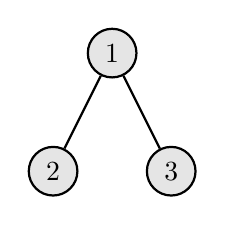
\begin{tikzpicture}
[every node/.style={draw, circle, minimum size=6mm, fill=gray!20!},  node distance=8mm,  thick]
\node{1}
child{node{2}}
child{node{3}};
\end{tikzpicture}
\end{figure}


\textbf{Output}: 25

\textbf{Explanation}:

The root-to-leaf path $1\longrightarrow 2$ represents the number $12$.

The root-to-leaf path $1\longleftrightarrow 3$ represents the number $13$.

Therefore, sum is $12 + 13 = 25$.
\end{flushleft}


\paragraph{Example 2:}

\begin{flushleft}
\begin{figure}[H]
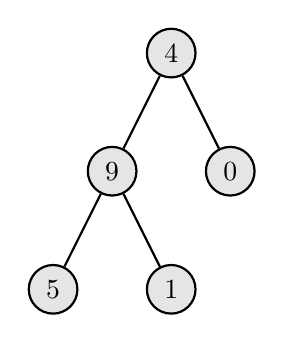
\begin{tikzpicture}
[every node/.style={draw, circle, minimum size=6mm, fill=gray!20!},  node distance=8mm,  thick]
\node{4}
child{node{9} child{node{5}} child{node{1}}}
child{node{0}};
\end{tikzpicture}
\end{figure}

\textbf{Output}: $1026$

\textbf{Explanation}:

The root-to-leaf path $ 4\longrightarrow9\longrightarrow5 $ represents the number $ 495 $.

The root-to-leaf path $4\longrightarrow 9\longrightarrow 1$ represents the number $ 491 $.

The root-to-leaf path $4\longrightarrow 0$ represents the number $ 40 $.

Therefore, sum is $495 + 491 + 40 = 1026$.
\end{flushleft}
\section{130 --- Surrounded Regions}
Given a 2D board containing \fcj{'X'} and \fcj{'O'} (the letter $O$), capture all regions surrounded by \fcj{'X'}.

A region is captured by flipping all \fcj{'O'}s into \fcj{'X'}s in that surrounded region.

\paragraph{Example:}

\begin{flushleft}


\[
\begin{bmatrix}
X & X & X & X\\
X & O & O & X\\
X & X & O & X\\
X & O & X & X
\end{bmatrix}
\]

After running your function, the board should be:

\[
\begin{bmatrix}
X & X & X & X\\
X & X & X & X\\
X & X & X & X\\
X & O & X & X
\end{bmatrix}
\]



\paragraph{Explanation:}

Surrounded regions shouldn't be on the border, which means that any \fcj{'O'} on the border of the board are not flipped to \fcj{'X'}. Any \fcj{'O'} that is not on the border and it is not connected to an \fcj{'O'} on the border will be flipped to \fcj{'X'}. Two cells are connected if they are adjacent cells connected horizontally or vertically.

\end{flushleft}


\subsection{Replace Border Os}
\begin{itemize}
\item Check the four border of the matrix. If there is a element is \fcj{'O'}, alter it and all its neighbor \fcj{'O'} elements to \fcj{'1'}.
\item Then, change all \fcj{'O'} to \fcj{'X'}
\item Finally, change back all the \fcj{'1'} to \fcj{'O'}
\end{itemize}

\setcounter{lstlisting}{0}
\begin{lstlisting}[style=customc, caption={Border Change First}]
void solve( vector<vector<char>>& board )
{
    //corner case
    if( board.empty() || ( board[0].empty() ) )
    {
        return;
    }
    auto M = board.size();
    auto N = board[0].size();
    //chech all four borders
    //flodd all 'O' to '1'
    for( size_t c = 0; c < N; ++c )
    {
        if( board[0][c] == 'O' )
        {
            flood( board, 0, c );
        }

        if( board[M - 1][c] == 'O' )
        {
            flood( board, M - 1, c );
        }
    }
    for( size_t r = 1; r < M - 1; ++r )
    {
        if( board[r][0] == 'O' )
        {
            flood( board, r, 0 );
        }

        if( board[r][N - 1] == 'O' )
        {
            flood( board, r, N - 1 );
        }
    }
    //change all 'O' to 'X'
    //change back '1' to 'O'
    for( size_t r = 0; r < M; ++r )
    {
        for( size_t c = 0; c < N; ++c )
        {
            if( board[r][c] == 'O' )
            {
                board[r][c] = 'X';
            }
            else if( board[r][c] == '1' )
            {
                board[r][c] = 'O';
            }
        }
    }
}
//flood 4 neighborhood for 'O'
void flood( vector<vector<char>>& board, size_t r, size_t c )
{
    if( board[r][c] == 'O' )
    {
        board[r][c] = '1';
    }
    else
    {
        return;
    }
    auto M = board.size();
    auto N = board[0].size();
    if( r + 1 < M )
    {
        flood( board, r + 1, c );
    }
    if( r >= 1 )
    {
        flood( board, r - 1, c );
    }
    if( c + 1 < N )
    {
        flood( board, r, c + 1 );
    }
    if( c >= 1 )
    {
        flood( board, r, c - 1 );
    }
}
\end{lstlisting}
\section{131 --- Palindrome Partitioning}
Given a string $s$, partition $s$ such that every substring of the partition is a palindrome.
\par
Return all possible palindrome partitioning of $s$.
\paragraph{Example:}
\begin{flushleft}
\textbf{Input}: \texttt{aab}
\\
\textbf{Output}:
\\
((\texttt{aa}, \texttt{b}), (\texttt{a}, \texttt{a}, \texttt{b}))
\end{flushleft}
因为需要找到所有的palindrome字符串,因此DFS是最自然的选择。在递归函数中,从给定的起始位置出发,然后逐个搜寻以这个起始位置为开始的string在后面哪个位置可以找到palindrome,如果找到了这个位置,把当前的substring加入当前的选择中,然后从找到的位置继续进行递归。

\setcounter{algorithm}{0}
\begin{algorithm}[H]
\caption{DFS}
\begin{algorithmic}[1]
\Procedure{Partition}{$S, L_S$}
\If{$L_s = 0$}
\State \Return \Comment Empty string
\EndIf
\State $P:=\emptyset$ \Comment The array to save all palindrome strings found in one pass
\State $\texttt{ans} := \emptyset$ \Comment The final result
\State $\texttt{DFS}(S, L_S, 0, P, \texttt{ans})$ \Comment The recursive helper function
\State \Return $\texttt{ans}$
\EndProcedure
\end{algorithmic}
\end{algorithm}
\texttt{DFS}从给定的位置$\alpha$出发,往后搜寻palindrome string。每找到一个,放入$P$中,然后从找到的string的末尾的下一个字符开始继续进行递归,递归结束后,将刚才加入的string从$P$中移除。当$\alpha=L_S$时,递归过程结束,将$P$插入到最终结果$A$中。
\begin{algorithm}[H]
\caption{DFS Helper Function}
\begin{algorithmic}[1]
\Function{DFS}{$S, L_S, \alpha, P, A$}
\If{$\alpha=L_S$}
\State $A\gets A+P$ 
\EndIf
\For{$i:=\alpha \to L_S-1$}
\State $l:=\alpha,\ r:=i+1$
\State $b:=\texttt{true}$ \Comment Indicate if $S[\alpha,\;i]$ is a palindrome or not
\While{$l < r$}
\If{$S[l]\neq S[r]$}
\State $b\gets \texttt{false}$ \Comment Not a palindrome string
\State \texttt{break}
\EndIf
\State $l\gets l+1$
\State $r\gets r-1$
\EndWhile
\If{$b=\texttt{true}$} \Comment $S[\alpha,\;i]$ is a palindrome
\State $P\gets P+S[\alpha,\;i]$ \Comment Add $S[\alpha,\;i]$ to current partition $P$
\State $\texttt{DFS}(S, L_S, i+1, P, A)$ \Comment Recursive on next character
\State $P\gets P-S[\alpha,\;i]$ \Comment Remove $S[\alpha,\;i]$ from current partition $P$
\EndIf
\EndFor
\EndFunction
\end{algorithmic}
\end{algorithm}
\section{132 --- Palindrome Partitioning II}
Given a string $s$, partition $s$ such that every substring of the partition is a palindrome.
\par
Return the minimum cuts needed for a palindrome partitioning of $s$.
\paragraph{Example:}
\begin{flushleft}
\textbf{Input}: \texttt{aab}
\\
\textbf{Output}: 1
\\
\textbf{Explanation}: The palindrome partitioning (aa, b) could be produced using 1 cut.
\end{flushleft}
\subsection{Dynamic Programming}
采用DP的方法需要构建两个array $F[i][j]$ and $C[i]$,$F[i][j]$ indicate $S[i,j]$是否是回文字符串,而$C[i]$则从$F[0][i]$中 find minimum cuts for $S[0,i-1]$。
\setcounter{algorithm}{0}
\begin{algorithm}[H]
\caption{Dynamic Programming}
\begin{algorithmic}[1]
\Procedure{MinCuts}{$S, L_S$}
\State Initialize array $F_{L_S\times L_S}$
\For{$i:=0\to L_S-1$}
\State $F[i][i] \gets 1$ \Comment Single character is definitely a palindrome
\EndFor
\For{$i:=0\to L_S-2$}
\If{$S[i]=S[i+1]$}
\State $F[i][i+1]\gets 1$
\EndIf
\EndFor
\For{$l:=3\to L_S$}
\For{$i:=0\to L_S-l+1$}
\State $j:=i+l-1$
\If{$S[i]=S[j]$}
\State $F[i][j]\gets 1$
\EndIf
\EndFor
\EndFor
\State Initialize array $C_{L_S}$
\algstore{132algo}
\end{algorithmic}
\end{algorithm}
\begin{algorithm}[H]
\begin{algorithmic}[1]
\algrestore{132algo}
\For{$i:=1\to L_S-1$}
\If{$F[0][i]=1$}
\State $C[i]=0$ \Comment $S[0,i]$ is a palindrome, no need to cut
\Else
\While{$j:=0\to i-1$}
\If{$F[j+1][i]=1$} \Comment $S[j+1, i]$ is a palindrome
\State $C[i]\gets \min(C[i], C[j]+1)$ \Comment Only need one more cut between $S[j]$ and $S[j+1]$
\EndIf
\EndWhile
\EndIf
\EndFor
\State \Return $C[L_S-1]$ \Comment $C[L_S-1]$ is the minimum cuts for $S[0,L_S-1]$
\EndProcedure
\end{algorithmic}
\end{algorithm}
\subsection{Manancher--Like Alogrithtm}
这种方法从左到右扫描$S$,在每一个位置$i$,只检查以$S[i]$为中心的substring。一旦找到一个substring不是palindrome,就会结束搜索,然后移动到下一个位置$i+1$。与DP方法类似,也需要一个array $C[i]$用来保存minimum cuts for $S[0, i]$。
\par
实现时,在每一个位置$i$,做两次循环,一次检查$S[i-j, i+j]$是否为palindrome,另外一个则检查$S[i-j-1,i+j]$是否为palindrome。循环的变量$j$从0开始,这样我们就能找到以$i$为中心的所有palindrome string,同时更新$C[i]$。一旦找到non-palindrome string,终止内部的这个循环,因为不会再出现以$i$为中心的palindrome string了。这可以避免很多在DP方法中不必要的palindrome检查。
\par
由于需要检查$i-j$和$i-j-1$是否大于零,这时候如果找到palindrome,我们需要直到$C[i-j-1]$和$C[[i-j-2]]$的值,这时候,$i-j-1$或者$i-j-2$都有可能小于零,因此为了方便起见,$C[i]$定义为minimum cuts for $S[0, i-1]$。因此$C[L]$就是所求之结果。如果$i=0$,那么$C[0]=-1$,这样$C$的长度就是$L_S+1$了。
\begin{algorithm}[H]
\caption{Manancher Algorithm}
\begin{algorithmic}[1]
\Procedure{MinCuts}{$S, L_S$}
\State Initialize array $C_{L_S+1}$
\For{$i:=0\to L_S$}
\State $C[i]\gets i-1$ \Comment The maximum cuts for palindrome partition is $l-1$
\EndFor
\For{$i:=1\to L$}
\State $j:=0$
\While{$i-j\geq 0$ \textbf{and} $i+j<L_S$} \Comment Odd length substring centered at $S[i]$
\If{$S[i-j]=S[i+j]$}
\State $C[i+j+1]\gets \min(C[i+j+1], 1 + C[i-j])$ \Comment One cut in $i-j$ and $i-j-1$
\Else
\State \texttt{break} \Comment Stop while loop
\EndIf
\State $j\gets j+1$
\EndWhile
\State $j\gets 0$ \Comment Reset $j$
\While{$i-j-1\geq 0$ \textbf{and} $i+j<L_S$} \Comment Even length substring centered at $S[i]$
\If{$S[i-j-1]=S[i+j]$}
\State $C[i+j+1]\gets \min(C[i+j+1], 1 + C[i-j-1])$ \Comment One cut in $i-j-1$ and $i-j-2$
\Else
\State \texttt{break} \Comment Stop while loop
\EndIf
\State $j\gets j+1$
\EndWhile
\EndFor
\State \Return $C[L_S]$ \Comment The minimum cuts for $S[0, L_S-1]$
\EndProcedure
\end{algorithmic}
\end{algorithm}

\section{133 --- Clone Graph}
Given the head of a graph $G$, return a deep copy (clone) of the graph. Each node in the graph contains a label $n$ and a list of its neighbors $A$. There is an edge $E$ between the given node and each of the nodes in its neighbors.
\subsection{DFS}
由于节点值是为唯一的,可以使用哈希表来对应节点值和新生成的节点。
\setcounter{algorithm}{0}
\begin{algorithm}[H]
\caption{DFS}
\begin{algorithmic}[1]
\Procedure{CloneGraph}{$G$}
\State $M:=\emptyset$ \Comment The hash map to map label to the new constructed node
\State $\texttt{ans}:=\texttt{DFS}(M, G)$
\State \Return \texttt{ans}
\EndProcedure
\end{algorithmic}
\end{algorithm}
\texttt{DFS}递归的copy以$G$为开始的graph。
\begin{algorithm}[H]
\caption{DFS Helper Function}
\begin{algorithmic}[1]
\Function{DFS}{$G, M$}
\If{$G=\texttt{null}$}
\State \Return $G$
\EndIf
\State $g:=\texttt{Label}(G)$ \Comment The label of node $G$
\If{$g\in M$}
\State \Return $M[g]$
\EndIf
\State Create a new node $\hat{G}$
\State $\texttt{Label}(\hat{G})\gets g$
\State $M[g]\gets \hat{G}$
\State $v:=\texttt{Neighbors}(G)$ \Comment The neighbors of $G$
\State $\hat{v}:=\texttt{Neighbors}(\hat{G})$ \Comment The neighbors of $\hat{G}$
\For{$i:=0\to |v|-1$}
\State $t:=\texttt{DFS}(v[i], M)$ \Comment Recursively copy $v[i]$
\State $\hat{v}\gets \hat{v} + t$ \Comment Add copy of $v[i]$ as one of neighbor of $\hat{G}$
\algstore{133algo}
\end{algorithmic}
\end{algorithm}
\begin{algorithm}[H]
\begin{algorithmic}[1]
\algrestore{133algo}
\EndFor
\EndFunction
\end{algorithmic}
\end{algorithm}
\subsection{BFS}
采用BFS时,可以用queue也可以用hash set然后swap 现在的level和下一个level。这里采用后者。同样需要一个hash map来记录label值和对应的新的clone node。有个tricky点是如果在map中找到了label对应的clone node,这个node就不用放到下一层去,否则会产生无限循环。
\begin{algorithm}[H]
\caption{BFS}
\begin{algorithmic}[1]
\Procedure{CloneGraph}{$G$}
\State $M:=\emptyset$ \Comment The hash map to map label to the new constructed node
\State $x:=\emptyset$ \Comment The current level of BFS tree
\State $x\gets x + G$ \Comment The first level contains only $G$
\State Create a clone node $G_c$
\State $\texttt{Label}(G_c)\gets \texttt{Label}(G)$
\While{$x\neq \emptyset$} \Comment BFS loop
\State $y:=\emptyset$ \Comment The hash set of next level
\For{$t \in x$}
\State $t_c:=M[\texttt{Label}(t)]$ \Comment Get the clone node in $M$
\State $v:=\texttt{Neighbors}(t_c)$
\For{$n \in \texttt{Neighbors}(t)$} \Comment Iterate over neighbor nodes of $t$
\If{$\texttt{Label}(n)\notin M$}
\State Create a new node $n_c$
\State $\texttt{Label}(n_c)\gets \texttt{Label}(n)$
\State $M[\texttt{Label}(n_c)]:=n_c$
\State $v\gets v+ n_c$ \Comment Add $n_c$ as one of neighbors of $t_c$
\State $y\gets y+n$ \Comment Add $n$ to next level
\Else \Comment $M$ contains the clone node of $\texttt{Label}(n)$
\State $v\gets v+M[\texttt{Label}(n)]$ \Comment Add the node as one of neighbors of $t_c$
\EndIf
\EndFor
\EndFor
\State $x\gets y$ \Comment Update $x$ as the next level
\algstore{133algo}
\end{algorithmic}
\end{algorithm}
\begin{algorithm}[H]
\begin{algorithmic}[1]
\algrestore{133algo}
\EndWhile
\State \Return $G_c$
\EndProcedure
\end{algorithmic}
\end{algorithm}

\section{134 --- Gas Station}
There are $N$ gas stations along a circular route, where the amount of gas at station i is $G[i]$.
\par
You have a car with an unlimited gas tank and it costs $C[i]$ of gas to travel from station $i$ to its next station $i+1$. You begin the journey with an empty tank at one of the gas stations.
\par
Return the starting gas station's index if you can travel around the circuit once in the clockwise direction, otherwise return $-1$.
\paragraph{Note:}
\begin{itemize}
\item If there exists a solution, it is guaranteed to be unique.
\item Both input arrays are non-empty and have the same length.
\item Each element in the input arrays is a non-negative integer.
\end{itemize}
\paragraph{Example 1:}
\begin{flushleft}
\textbf{Input}:
\\
$G  = [1,2,3,4,5]$, $C =[3,4,5,1,2]$
\\
\textbf{Output}: 3
\\
\textbf{Explanation}:
\begin{itemize}
\item Start at station 3 (index 3) and fill up with 4 unit of gas. Your tank $= 0 + 4 = 4$
\item Travel to station 4. Your tank $= 4 - 1 + 5 = 8$
\item Travel to station 0. Your tank $= 8 - 2 + 1 = 7$
\item Travel to station 1. Your tank $= 7 - 3 + 2 = 6$
\item Travel to station 2. Your tank $= 6 - 4 + 3 = 5$
\item Travel to station 3. The cost is 5. Your gas is just enough to travel back to station 3.
\end{itemize}
Therefore, return 3 as the starting index.
\end{flushleft}
\paragraph{Example 2:}
\begin{flushleft}
\textbf{Input}:
\\ 
$G  = [2,3,4]$, $C = [3,4,3]$
\\
\textbf{Output}: $-1$
\\
\textbf{Explanation}:
\begin{itemize}
\item You cannot start at station 0 or 1, as there is not enough gas to travel to the next station.
\item Let's start at station 2 and fill up with 4 unit of gas. Your tank $= 0 + 4 = 4$
\item Travel to station 0. Your tank $= 4 - 3 + 2 = 3$
\item Travel to station 1. Your tank $= 3 - 3 + 3 = 3$
\item You cannot travel back to station 2, as it requires 4 unit of gas but you only have 3.
\end{itemize}
Therefore, you cannot travel around the circuit once no matter where you start.
\end{flushleft}
\subsection{Analysis}
首先能走完整个环的前提是gas的总量要大于cost的总量,这样才会有起点的存在。假设开始设置起点$s = 0$, 并从这里出发,如果当前的gas值大于cost值,就可以继续前进,此时到下一个station,剩余的gas加上当前的gas再减去cost,看是否大于0,若大于0,则继续前进。当到达某一个station时,若这个值小于0了,则说明从起点到这个点中间的任何一个点都不能作为起点,则把起点设为下一个点,继续遍历。当遍历完整个环时,当前保存的起点即为所求。
\setcounter{algorithm}{0}
\begin{algorithm}[H]
\caption{One Pass}
\begin{algorithmic}[1]
\Procedure{CanCompleteCircuit}{$G,C,L$}
\State $t:=0$ \Comment Total sum of difference between gas and cost at each station
\State $s:=0$ \Comment The start station
\State $z:=0$ \Comment Current sum of difference between gas and cost at each station
\For{$i:=0\to L$} \Comment $G$ and $C$ lengths are equal to $L$
\State $t\gets t + G[i] - C[i]$
\State $z\gets z + G[i] - C[i]$
\If{$z<0$} 
\State $z\gets 0$ \Comment Reset to zero
\State $s\gets i+1$ \Comment Move start station to next
\EndIf
\EndFor
\If{$t<0$} \Comment Total gass are less than total costs
\State \Return $-1$ \Comment Cannot complete the circuit
\Else
\State \Return $z$
\EndIf
\EndProcedure
\end{algorithmic}
\end{algorithm}

\section{135 --- Candy}
There are $N$ children standing in a line. Each child is assigned a rating value.
\par
You are giving candies to these children subjected to the following requirements:
\begin{enumerate}
\item Each child must have at least one candy.
\item Children with a higher rating get more candies than their neighbors.
\item What is the minimum candies you must give?
\end{enumerate}
\paragraph{Example 1:}
\begin{flushleft}
\textbf{Input}: \fcj{[1,0,2]}
\\
\textbf{Output}: 5
\\
\textbf{Explanation}: You can allocate to the first, second and third child with 2, 1, 2 candies respectively.
\end{flushleft}
\paragraph{Example 2:}
\begin{flushleft}
\textbf{Input}: \fcj{[1,2,2]}
\\
\textbf{Output}: 4
\\
\textbf{Explanation}: You can allocate to the first, second and third child with 1, 2, 1 candies respectively. The third child gets 1 candy because it satisfies the above two conditions.
\end{flushleft}
\subsection{Brute Force}
这是最直接的方法,首先创建一个1维数组$C$用来跟踪分配的candies。
\begin{itemize}
\item 首先,给每个student一个candy。然后从左至右扫描$C$。对于每个位置,如果其rating $R[i]$ 比左边的大,即$R[i]>R[i-1]$,并且$C[i]\leq C[i-1]$,那么就要update $C[i]$为$C[i-1]+1$。
\item 同样的,我们也需要检查其rating是否比右边的大,即$R[i]>R[i+1]$,如果是,并且$C[i] \leq C[i+1]$,那么$C[i]$还要被再次update为$C[i+1]+1$。
\item 继续上述步骤直到没有发生任何update $C[i]$的操作。
\item 最后将数组$C$中的元素加起来就是最终的结果。
\end{itemize}
\subsection{Using One Array}
上述Brute Force的方法虽然直接,但是效率不高。为了提高效率,首先用两个1维数组$L$ and $R$。$L$用来保存从左至右所需要的candies的数量,即如果当前student的rating比其左边的高,他应该得到比左边更多的candies。类似的,$R$就是保存从右至左所需要的candies的数量,即如果当前student的rating比其右边的高,他应该得到比右边更多的candies。
\par
开始时,$L$ and $R$中都是1, 即每个student都是1个candy。首先从左到右遍历ratings数组$A$,在当前位置$i$,如果$A[i]>A[i-1]$,那么$L[i]\gets L[i-1]+1$。因为$L[i]$在update前总是小于或者等于$L[i-1]$的。
\par
接着从右到左遍历$R$,类似的在当前位置$i$,如果$A[i]>A[i+1]$,那么$R[i]\gets R[i+1]+1$。
\par
这时候,在位置$i$处,需要得到$\max(L[i],R[i])$以满足左右两侧rating的大小关系。因此最后的minimum number of candies就是
\[
\sum_{0}^{|A|-1}\max(L[i], R[i])
\]
不过在从右到左时,可以不用$R$数组,直接更新$L[i]$为$\max(L[i], L[i+1]+1)$即可。这样就只需要一个数组了。

\setcounter{lstlisting}{0}
\begin{lstlisting}[style=customc, caption={Bidirectional Scanning}]
int candy( vector<int>& ratings )
{
    auto L( static_cast< int >( ratings.size() ) );
    vector<int> candies( ratings.size(), 1 );
    //scan from left to right
    //to check left side of each person
    for( auto i = 1; i < L; ++i )
    {
        if( ratings[i] > ratings[i - 1] )
        {
            //person i need more candies than person i-1
            candies[i] = candies[i - 1] + 1;
        }
    }
    //scan from right to left
    //to check right side of each person
    auto ans( 0 );
    for( auto i = L - 2; i >= 0; --i )
    {
        if( ratings[i] > ratings[i + 1] )
        {
            //person i need more candies than person i+1
            candies[i] = ( max )( candies[i], candies[i + 1] + 1 );
        }
        ans += candies[i];
    }
    //we have not added the last person's candies.
    ans += candies.back();
    return ans;
}
\end{lstlisting}

\subsection{One Pass With Constant Space}
上述方法仍然需要线性空间。如果不需要线性空间,那么首先需要观察到如下信息:
\begin{itemize}
\item 分配candies都是按1递增进行的。因为目标是最少的candies。
\item 分配candies,local minimum处的student得到的candy必须是1。
\end{itemize}
因此分配candy要么是以$1,2,3,\ldots,n$的形式,或者是$n, n-1, \ldots, 2, 1$的形式,这两种形式的和都是$n\times(n+1)/2$。

因此我们可以将ratings array看作是由一些上坡和下坡部分构成的。当在上坡的时候,candy的分配就是$1,2,3,\ldots,n$的形式。类似的,下坡的分配形式就是$k, k-1, \ldots, 2,1$。现在的问题就是local maximum或者说local peak到底应该包含在上坡或者下坡的哪一个中?很明显,为了同时大于左右两侧的candy数量,local peak所赋予的candy数必须由其所在上坡和下坡中的长度最长的那个来决定。而对于local valley即波谷,我们把它包含在下一个上坡段中,其所assign的candy数量必当为1( which can be subtracted from the next slope's count calculation )

在实现时, maintain当前段和上一段的类型即是上坡还是下坡。另外keep track上坡和下坡的长度,即所包含的element的个数。当遇到如下情形时,
\begin{enumerate}
\item 一段上坡,然后紧接着是相等的rating
\item 一段下坡,然后紧接着是一段上坡
\item 一段下坡,然后紧接着是相等的rating
\end{enumerate}
这时候,就需要更新当前当前所分配的candy的总的数量。


\begin{lstlisting}[style=customc, caption={Up And Down Slope}]
int candy( vector<int>& ratings )
{
    if( ratings.size() <= 1ULL )
    {
        return ratings.empty() ? 0 : 1;
    }
    int candies = 0;
    int up_count = 0;
    int down_count = 0;
    unsigned char last_slope( 0 );
    //helper lambad to get (1+..+count)
    auto sum = []( int count )
    {
        return ( count * ( count + 1 ) ) / 2;
    };
    for( auto i = 1ull; i < ratings.size(); ++i )
    {
        unsigned char cur_slope( 0 );
        if( ratings[i] > ratings[i - 1] )
        {
            //up slope
            cur_slope = 1;
        }
        else if( ratings[i] < ratings[i - 1] )
        {
            //down slope
            cur_slope = 2;
        }

        //find end of mountain point
        //a mountain contains a up slope and a down slope
        //or a up slope with leveling
        bool end_mountain = false;
        if( ( last_slope == 1 ) && ( cur_slope == 0 ) )
        {
            //up and then level
            end_mountain = true;
        }
        else if( ( last_slope == 2 ) && ( cur_slope < 2 ) )
        {
            //down and then level or up
            end_mountain = true;
        }

        if( end_mountain )
        {
            //the candies in each mountain
            //will have candies for up slope and down slope
            //and the candies for the local peak which is ( max )( up_count, down_count ) + 1
            //but we ignore 1 here because we the end of moutain
            //is local valley and it will be used as the next start of mountain
            candies += sum( up_count ) + sum( down_count ) + ( max )( up_count, down_count );
            up_count = 0;
            down_count = 0;
        }
        switch( cur_slope )
        {
        case 1:
            //this is up slope, increments the length of up counts
            ++up_count;
            break;

        case 2:
            //this is down slope, increments the length of down counts
            ++down_count;
            break;

        case 0:
            //this is leveling, just increments the candies
            ++candies;
            break;
        }

        last_slope = cur_slope;

    } //end for
    //process last segment containing turning point
    //in this case, we have to add 1 to ( max )( up_count, down_count )
    //because this end of mountain is the final local valley
    candies += sum( up_count ) + sum( down_count ) + ( max )( up_count, down_count ) + 1;
    return candies;
}
\end{lstlisting}

\section{136 --- Single Number}
Given a non-empty array of integers $A$, every element appears twice except for one. Find that single one.
\paragraph{Note}: 
\begin{itemize}
\item Your algorithm should have a linear runtime complexity. Could you implement it without using extra memory?
\end{itemize}

\paragraph{Example 1:}
\begin{flushleft}
\textbf{Input}: $[2,2,1]$
\\
\textbf{Output}: 1
\end{flushleft}
\paragraph{Example 2:}
\textbf{Input}: $[4,1,2,1,2]$
\\
\textbf{Output}: 4
\subsection{XOR}
Very easy problem.  XOR all numbers together to find the unique number.
\section{137 --- Single Number II}
Given a non-empty array of integers $A$, every element appears three times except for one, which appears exactly once. Find that single one.
\paragraph{Note:}
\begin{flushleft}
Your algorithm should have a linear runtime complexity. Could you implement it without using extra memory?
\end{flushleft}
\paragraph{Example 1:}
\begin{flushleft}
\textbf{Input}: $[2,2,3,2]$
\\
\textbf{Output}: 3
\end{flushleft}
\paragraph{Example 2:}
\begin{flushleft}
\textbf{Input}: $[0,1,0,1,0,1,99]$
\\
\textbf{Output}: 99
\end{flushleft}
\subsection{Bitwise Operation}
首先问题可以推广到如下形式,给定一个array $A$,其中除了一个数字重复了$p$次,其余的都重复了$k$次,找出这个重复$p$次的数字。
\par
首先从简单的例子开始,假定有一组1-bit数字构成的array $A$, 用一个counter记录array中数字1的出现次数,当这个counter到达某个值$k$时,就重置为0,然后继续。
\par
很明显,如果这个counter能够计数到$k$,假设其有$m$个bits,那么就有$2^m\geq k$,变换一下也就是$m\geq \log_{2}(k)$。
\par
现在来看当遍历数组$A$时,counter的每个bit是如何变化的,假设counter的$m$个bits从最高位到最低位分别为$b_{m-1}, \ldots, b_0$,由于当遇到数字0时,counter是保持不变的,那么具有如此性质的bitwise操作只有\textbf{OR}或者是\textbf{XOR}。接下来看这两种操作哪一种最佳。
\par
最开始,counter中的所有bit都是0。 直到遇到数字1,这些bits才开始发生改变。当遇到第一个1时,这时候$b_{m-1}=0,\ldots, b_0=1$。当遇到第二个1时,则变化为$b_{m-1}=0,\ldots, b_1=1, b_0=0$。注意到,$b_0$变成了0。如果用OR操作,那么$b_0\gets b_0\;\texttt{or}\; i$,这时候$b_0$仍然是1。因此,只能选择异或操作。对于$b_1,\ldots,b_{m-1}$,需要找到在什么样的情况下这些bits会发生改变。比如以$b_1$为例,当遇到数字1,这时候$b_0$必须是1才会使得我们必须改变$b_1$的值。因为如果是0,只需要把$b_0$从0变为1即可,并不需要改变$b_1$的值。因此$b_1$只有在$b_0$和$i$都是1的情况下才会改变其值,写成bitwise的形式就是$b_1\gets b_1\;\texttt{XOR}\;(b_0\;\texttt{AND}\;i)$。以此类推,$b_{m-1}$只有当$b_{m-2},\ldots,b_1,b_0$和$i$都是1的情况下才会需要改变,即$b_{m-1}\gets b_{m-1}\;\texttt{XOR}\;(b_{m-2}\;\texttt{AND}\;\ldots\;\texttt{AND}\;b_0\;\texttt{AND}\;i)$。这就是所需要的bitwise operation。
\par
上述bitwise operation是从0一直到$2^{m}-1$,而不是$k$。如果$k<2^m-1$,则需要在counter等于$k$时,将counter重置为0。要做到这一点,需要用一个mask $M$ 来和$b_{m-1},\ldots, b_0$做\texttt{AND} operation,即
\begin{align*}
b_{m-1}&\gets b_{m-1}\;\texttt{AND}\;M\\
b_{m-2}&\gets b_{m-2}\;\texttt{AND}\;M\\
\ldots& \\
b_0&\gets b_0\;\texttt{AND}\;M
\end{align*}
而$M$只有当counter等于$k$时才等于0,其他情况下都为1。假设$k$写成二进制的形式位$x_{m-1}, \ldots, x_{0}$,那么这个mask可以按照如下方法得到
\[
\texttt{NOT}(y_0\;\texttt{AND}\;y_1\;\texttt{AND}\ldots\texttt{AND}\;y_{m-1})
\]
其中$y_i=b_i$ when $x_j=1$,$y_i=\texttt{NOT}(b_i)$ when $x_i=0$。这里$i\in[0,m-1]$。
\par
例如$k=3$,写成二进制形式为$11$,即$x_{1}=1,x_0=1$。那么mask就是$\texttt{NOT}(b_1\;\texttt{AND}\;b_0)$。因此算法的框架就像下面所示的那样
\setcounter{algorithm}{0}
\begin{algorithm}[H]
\caption{Overall Description}
\begin{algorithmic}[1]
\Procedure{F}{$A, L$}
\For{$i:=0\to L-1$}
\State $n:=A[i]$
\State $b_{m-1}\gets b_{m-1}\;\texttt{XOR}\;(b_{m-2}\;\texttt{AND}\ldots\texttt{AND}\;b_0\;\texttt{AND}\;n)$
\State $b_{m-2}\gets b_{m-2}\;\texttt{XOR}\;(b_{m-3}\;\texttt{AND}\ldots\texttt{AND}\;b_0\;\texttt{AND}\;n)$
\State $\ldots$
\State $b_{0}\gets b_{0}\;\texttt{XOR}\;n$
\State $M:=\texttt{NOT}(y_0\;\texttt{AND}\ldots\texttt{AND}\;y_{m-1})$ \Comment The mask
\State $x_{m-1}\gets x_{m-1}\;\texttt{AND}\;M$
\State $x_{m-2}\gets x_{m-2}\;\texttt{AND}\;M$
\State $\ldots$
\State $x_{0}\gets x_{0}\;\texttt{AND}\;M$
\EndFor
\EndProcedure
\end{algorithmic}
\end{algorithm}
假设$A$中的number都是32bit整数。最直接的方法当然是对于整数中的32个bit分别创建1个counter,也就是有32个counters。不过更好的方法用$m$个32位整数而不是32个$m$位整数,这里$m$是满足$m\geq\log_2{k}$的最小整数。也就是说可以把32个counter的同一个bit分别单独拿出来构成一个整数,这样就只需要$m$个32位整数了,如下图所示
\begin{figure}[H]
\includegraphics[width=15cm]{137.png}
\end{figure}
有了这$m$个32位整数$m_0, m_1,\ldots, m_{31}$,以$m_0$为例,它是一个32bit整数。当遍历完整个array时,$m_0$中的第$z$个bit将由array中所有number的第$z$个bit位确定。如果一个number的第$z$个bit位在array中出现了$k$的倍数次,那么当计数到$k$时,由于我们要将counter重置为0,这个number在第$z$个bit也会重置为0。因此只有那个重复了$p$次的number在第$z$个bit位出现次数才最终决定了这个位上的值。由于这个number的出现次数是$p$,那么$p\bmod k\neq0$。当$p>k$时,只有$p\bmod k$次才最终决定在$z$处的值。也就是说在这个number对于第$z$个bit位而言其有效的重复次数是$\hat{p}:=p\bmod k$。
\par
假设这个有效次数$\hat{p}$写成二进制形式位$\hat{p}_{m-1}\hat{p}_{m-2}\ldots\hat{p}_0$,那么如果$m_i$也就是第$i$个counter的第$z$个bit是1,很显然那个重复了$p$的number的有效次数$\hat{p}$的第$z$个bit也为1。而如果$m_i$的第$z$个bit位是0,那么重复了$p$次的数字的有效次数$\hat{p}$的第$z$个bit只能是0。如果是1,那么因为在遍历完整个数组后,这个位上的1出现了$\hat{p}$次,最终结果还是1,就不是我们假设的0了。而这个$z$是从0到32的,因此结论就是如果$\hat{p}_i=1$,那么$m_i$就是那个重复了$p$次的数字。
\par
因此算法首先计算出$\hat{p}:=p\bmod k$,然后只要$\hat{p}$的第$z$个bit位为1, 就返回$m_z$,如果有多个这样的bit位,返回其中任意一个即可。
\par
\begin{itemize}
\item 当$k=2$, $p=1$时, 只需要$m=1$个32位整数作为counter,因为$2^1\geq2$,而因为$2^m=k$,甚至都不要mask。因此算法其实就是每个数进行\texttt{XOR}。
\item 当$k=3$, $p=1$时,由于$2^2>3$,因此$m=2$,即两个32位整数的counter$m_0$ and $m_1$。而$2^m=2^2=4>k=3$,因此需要mask $M$。$k$的二进制形式为$k=b(11)$,因此$M = \texttt{NOT}(m_0\;\texttt{AND}\;m_1)$。算法如下所示:
\end{itemize}
\setcounter{algorithm}{0}
\begin{algorithm}[H]
\caption{K=3 AND P=1}
\begin{algorithmic}[1]
\Procedure{F}{$A, L$}
\State $m_0:=0$, $m_1:=0$, $M:=0$
\For{$i:=0\to L-1$}
\State $n:=A[i]$
\State $m_1\gets m_1\;\texttt{XOR}\;(m_0\;\texttt{AND}\;n)$
\State $m_0\gets m_0\;\texttt{XOR}\;n$
\State $M\gets \texttt{NOT}(m_0\;\texttt{AND}\;m_1)$
\State $m_1\gets m_1\;\texttt{AND}\;M$
\State $m_0\gets m_0\;\texttt{AND}\;M$
\EndFor
\State \Return $m_0$
\EndProcedure
\end{algorithmic}
\end{algorithm}
由于$p\bmod k=1$,因此返回$m_0$。
\begin{itemize}
\item 当$k=5$, $p=3$时, $m=\lfloor\log_25\rfloor=3$。因此需要3个counter,$m_0$,$m_1$ and $m_2$。而$p\bmod k=3$,二进制形式为$b(011)$,因此返回$m_0$或者$m_1$都可以。而$k$的二进制是$b(101)$,因此$M:=\texttt{NOT}(m_2\;\texttt{AND}\;\texttt{NOT}(m_1)\;\texttt{AND}\;m_0)$
\end{itemize}


\section{138 --- Copy List with Random Pointer}
\definecolor{gray1}{RGB}{229,229,229}
\definecolor{blue1}{RGB}{178,214,239}
\definecolor{red1}{RGB}{255,187,177}
\definecolor{red2}{RGB}{201,45,57}
\definecolor{blue2}{RGB}{12,124,186}
A linked list $L$ is given such that each node contains an additional random pointer which could point to any node in the list or \texttt{null}.

Return a deep copy of the list.
\subsection{Recursive}
Lets first look at how the linked list looks like
\begin{figure}[H]
\begin{tikzpicture}
[graynode/.style={draw,rectangle,minimum width=10mm, minimum height=8mm, fill=gray1},
rednode/.style={draw,rectangle,minimum width=10mm, minimum height=8mm, fill=red1},
bluenode/.style={draw,rectangle,minimum width=10mm, minimum height=8mm, fill=blue1},
]
\node(){};
\node[graynode](1) {4};
\node[rednode](2) [anchor=west] at (1.east) {};
\node[bluenode](3) [anchor=west] at (2.east) {};
\node[graynode](1a) [right=12mm of 3] {7};
\node[rednode](2a) [anchor=west] at (1a.east) {};
\node[bluenode](3a) [anchor=west] at (2a.east) {};
\node[graynode](1b) [right=12mm of 3a] {$-2$};
\node[rednode](2b) [anchor=west] at (1b.east) {};
\node[bluenode](3b) [anchor=west] at (2b.east) {};
\draw[fill=red2](2.center) circle [radius=1.5mm];
\draw[>=stealth,->,red2, line width=0.5mm] (2.center) to [out=60] (1b.north);
\draw[fill=red2](2a.center) circle [radius=1.5mm];
\draw[>=stealth,->,red2, line width=0.5mm] (2a.center) to [out=-80, in=-60] (1.south);
\draw[fill=blue2](3.center) circle [radius=1.5mm];
\draw[>=stealth,->,blue2, line width=0.5mm] (3.center) to (1a.west);
\draw[fill=blue2](3a.center) circle [radius=1.5mm];
\draw[>=stealth,->,blue2, line width=0.5mm] (3a.center) to (1b.west);
\draw[fill=red2] (2b.center) circle [radius=1.5mm];
\draw[fill=blue2] (3b.center) circle [radius=1.5mm];
\node (n1) [below=4mm of 2b] {\small None};
\draw[>=stealth,->,red2,line width=0.5mm] (2b.center) to (n1);
\node (n2) [below=4mm of 3b] {\small None};
\draw[>=stealth,->,blue2,line width=0.5mm] (3b.center) to (n2);
\node[draw, rectangle, minimum size=6mm, fill=red1] (random) [below=22mm of 3, xshift=3mm] {};
\node[minimum size=6mm] (exp1) [right=1mm of random] {\footnotesize Random Pointer};
\node[draw, rectangle, minimum size=6mm, fill=blue1] (np) [below=22mm of 3a, xshift=3mm] {};
\node[minimum size=6mm] (exp2) [right=1mm of np] {\footnotesize Next Pointer};
\end{tikzpicture}
\end{figure}
In the above diagram, for a given node the \textcolor{blue}{next} pointer points to the next node in the linked list. The next pointer is something standard for a linked list and this is what \textbf{links} the nodes together. What is interesting about the diagram and this problem is the \textcolor{blue}{random} pointer which, as the name suggests can point to any node in the linked list or can be a null.

The basic idea behind the recursive solution is to consider the linked list like a \textbf{graph}. Every node of the Linked List has 2 pointers (edges in a graph). Since, random pointers add the randomness to the structure we might visit the same node again leading to cycles.
\begin{figure}[H]
\begin{tikzpicture}
[graynode/.style={draw,rectangle,minimum width=10mm, minimum height=8mm, fill=gray1},
rednode/.style={draw,rectangle,minimum width=10mm, minimum height=8mm, fill=red1},
bluenode/.style={draw,rectangle,minimum width=10mm, minimum height=8mm, fill=blue1},
]
\node(){};
\node[graynode](1) {\textbf{4}};
\node[rednode](2) [anchor=west] at (1.east) {};
\node[bluenode](3) [anchor=west] at (2.east) {};
\node[graynode](1a) [right=12mm of 3] {7};
\node[rednode](2a) [anchor=west] at (1a.east) {};
\node[bluenode](3a) [anchor=west] at (2a.east) {};
\draw[fill=red2](2a.center) circle [radius=1.5mm];
\draw[>=stealth,->,red2, line width=0.5mm] (2a.center) to [out=-80, in=-60] (1.south);
\draw[fill=blue2](3.center) circle [radius=1.5mm];
\draw[>=stealth,->,blue2, line width=0.5mm] (3.center) to (1a.west);
\node[draw, rectangle, minimum size=6mm, fill=red1] (random) [below=22mm of 1, xshift=3mm] {};
\node[minimum size=6mm] (exp1) [right=1mm of random] {\footnotesize Random Pointer};
\node[draw, rectangle, minimum size=6mm, fill=blue1] (np) [below=22mm of 1a, xshift=3mm] {};
\node[minimum size=6mm] (exp2) [right=1mm of np] {\footnotesize Next Pointer};
\end{tikzpicture}
\end{figure}
In the diagram above we can see the random pointer points back to the previously seen node hence leading to a cycle. We need to take care of these cycles in the implementation.
\par
All we do in this approach is to just traverse the graph and clone it. Cloning essentially means creating a new node for every unseen node you encounter. The traversal part will happen recursively in a depth first manner. Note that we have to keep track of nodes already processed because, as pointed out earlier, we can have cycles because of the random pointers.
\par
The steps of the algorithm implementation include
\begin{enumerate}
    \item Start traversing the graph from \textcolor{red}{head} node. Since we view the list as a graph, below is the graph representation of the above linked list example.
\begin{figure}[H]
\begin{tikzpicture}
[graynode/.style={draw,rectangle,minimum width=10mm, minimum height=8mm, fill=gray1},
rednode/.style={draw,rectangle,minimum width=10mm, minimum height=8mm, fill=red1},
bluenode/.style={draw,rectangle,minimum width=10mm, minimum height=8mm, fill=blue1},
]
\node[draw, ellipse, minimum height = 3cm, minimum width = 4.2cm, fill=gray1] (node1) {};
\node[rednode](2) [anchor=center] at (node1.center) {};
\node[graynode](1) [anchor=east] at (2.west) {\textbf{4}};
\node[bluenode](3) [anchor=west] at (2.east) {};
\draw[fill=red2] (2.center) circle [radius=1.5mm];
\draw[fill=blue2] (3.center) circle [radius=1.5mm];
\node (A) [above=1mm of 2] {\small \textbf{A}};
\node (S) [above=7mm of node1] {\small \textbf{Head}};
\draw[>=stealth,->,line width=0.5mm] (S.south) to (node1.north);
%node 2 south west
\node[draw, ellipse, minimum height = 3cm, minimum width = 4.2cm, fill=gray1] (node2) [below=2.8cm of node1, xshift=-4.0cm] {};
\node[rednode](2a) [anchor=center] at (node2.center) {};
\node[graynode](1a) [anchor=east] at (2a.west) {\textbf{7}};
\node[bluenode](3a) [anchor=west] at (2a.east) {};
\draw[fill=red2] (2a.center) circle [radius=1.5mm];
\draw[fill=blue2] (3a.center) circle [radius=1.5mm];
\node (A) [above=1mm of 2a] {\small \textbf{B}};
%node 3 south east
\node[draw, ellipse, minimum height = 3cm, minimum width = 4.2cm, fill=gray1] (node3) [below=2.8cm of node1, xshift=4.0cm] {};
\node[rednode](2b) [anchor=center] at (node3.center) {};
\node[graynode](1b) [anchor=east] at (2b.west) {$\mathbf{-2}$};
\node[bluenode](3b) [anchor=west] at (2b.east) {};
\draw[fill=red2] (2b.center) circle [radius=1.5mm];
\draw[fill=blue2] (3b.center) circle [radius=1.5mm];
\node (A) [above=1mm of 2b] {\small \textbf{C}};
%draw arrows node1 between node2
\path[name path=e1] (node1.center) ellipse (2.1cm and 1.5cm);
\path[name path=e2] (node2.center) ellipse (2.1cm and 1.5cm);
\path[name path=l1] (2.center) -- (2a.center);
\path[name path=l2] (1.center) -- (1a.center);
\path[name intersections={of=e1 and l1, by=I1}];
\path[name intersections={of=e2 and l1, by=I2}];
\path[name intersections={of=e1 and l2, by=I3}];
\path[name intersections={of=e2 and l2, by=I4}];
\coordinate (t1) at (I1);
\coordinate (t2) at (I2);
\coordinate (t3) at (I3);
\coordinate (t4) at (I4);
\draw[>=stealth,->,line width=0.5mm,red2] (t2) -- (t1);
\draw[>=stealth,->,line width=0.5mm,blue2] (t3) -- (t4);
%draw arrows node2 to node3
\draw[>=stealth,->,line width=0.5mm,blue2] (node2) -- (node3);
%draw arrows node1 to node3
\draw[>=stealth,->,line width=0.5mm,red2] (node1) -- (node3);
%draw explain random pointer
\node[draw, rectangle, minimum size=6mm, fill=red1] (random) [below=15mm of node2, xshift=-6mm] {};
\node[minimum size=6mm] (exp1) [right=1mm of random] {\footnotesize Random Pointer};
%draw explain next pointer
\node[draw, rectangle, minimum size=6mm, fill=blue1] (np) [below=15mm of node3, xshift=-9mm] {};
\node[minimum size=6mm] (exp2) [right=1mm of np] {\footnotesize Next Pointer};
\end{tikzpicture}
\end{figure}
    In the above example, \textcolor{red}{head} is where we begin our graph traversal.
    \item If we already have a cloned copy of the current node in the visited dictionary, we use the cloned node reference.
    \item If we don't have a cloned copy in the visited dictionary, we create a new node and add it to the visited dictionary.
    \item We then make \textbf{two recursive calls}, one using the random pointer and the other using next pointer. The diagram from step 1, shows random and next pointers in red and blue color respectively. Essentially we are making recursive calls for the children of the current node. In this implementation, the children are the nodes pointed by the random and the next pointers.
\end{enumerate}

\setcounter{lstlisting}{0}
\begin{lstlisting}[style=customc, caption={DFS}]
Node* copyRandomList( Node* head )
{
    unordered_map<Node*, Node*> m;
    return do_copy( head, m );
}
Node* do_copy( Node* node, unordered_map<Node*, Node*>& m )
{
    if( !node )
    {
        return nullptr;
    }
    auto it = m.find( node );
    if( it != m.end() )
    {
        return it->second;
    }
    //create the clone node of current node
    auto clone = new Node( node->val, nullptr, nullptr );
    //we need to add to map first
    m.emplace( node, clone );
    //deep copy node->next;
    clone->next = do_copy( node->next, m );
    //deep copy node->random
    clone->random = do_copy( node->random, m );
    return clone;
}
\end{lstlisting}

%This approach does not model the linked list as a graph, instead simply treat it as it is. When we are iterating over the list, we can create new nodes via the random pointer or the next pointer whichever points to a node that doesn't exist in our visited dictionary.
%\par
%The overall algorithm takes following steps
%\begin{enumerate}
%    \item Traverse the linked list starting at \textcolor{red}{head} of the linked list.
%%        \begin{figure}[H]
%%        \centering
%%        \includegraphics[width=12cm]{138-4.png}
%%        \end{figure}
%    In the above diagram we create a new \textbf{cloned} \textcolor{red}{head} node. The cloned node is shown using dashed lines. In the implementation we would even store the reference of this newly created node in a visited dictionary.
%    \item Random Pointer
%    \begin{itemize}
%        \item If the \textcolor{red}{random} pointer of the current node $i$ points to the a node $j$ and a clone of $j$ already exists in the visited dictionary, we will simply use the cloned node reference from the visited dictionary.
%        \item If the \textcolor{red}{random} pointer of the current node $i$ points to the a node $j$ which has not been created yet, we create a new node corresponding to $j$ and add it to the visited dictionary.
%    \end{itemize}
%%        \begin{figure}[H]
%%        \centering
%%        \includegraphics[width=12cm]{138-5.png}
%%        \end{figure}    
%    In the above diagram the \textcolor{red}{random} pointer of node $A$ points to a node $C$. Node $C$ which was not visited yet as we can see from the previous diagram. Hence we create a new cloned $C^{'}$ node corresponding to node $C$ and add it to visited dictionary.
%    \item Next Pointer
%    \begin{itemize}
%        \item If the \textcolor{red}{next} pointer of the current node $i$ points to the a node $j$ and a clone of $j$ already exists in the visited dictionary, we will simply use the cloned node reference from the visited dictionary.
%        \item If the \textcolor{red}{next} pointer of the current node $i$ points to the a node $j$ which has not been created yet, we create a new node corresponding to $j$ and add it to the visited dictionary.
%    \end{itemize}
%%        \begin{figure}[H]
%%        \centering
%%        \includegraphics[width=12cm]{138-6.png}
%%        \end{figure}     
%    In the above diagram the \textcolor{red}{next} pointer of node $A$ points to a node $B$. Node $B$ which was not visited yet as we can see from the previous diagram. Hence we create a new cloned $B^{'}$ node corresponding to node $B$ and add it to visited dictionary.
%    \item We repeat steps 2 and 3 until we reach the end of the linked list.
%    In the above diagram, the \textcolor{red}{random} pointer of node $B$ points to an already visited node $A$. Hence in step 2, we don't create a new copy for the clone. Instead we point \textcolor{red}{random} pointer of cloned node $B^{'}$  to already existing cloned node  $A^{'}$.
%    \par
%    Also, the \textcolor{red}{next} pointer of node $B$ points to an already visited node $C$. Hence in step 3, we don't create a new copy for the clone. Instead we point \textcolor{red}{next} pointer of cloned node $B^{'}$ to already existing cloned node $C^{'}$.
%\end{enumerate}
%\begin{algorithm}[H]
%\caption{Iterative With O(n) Memory}
%\begin{algorithmic}[1]
%\Procedure{CopyRandomList}{$L$}
%\If{$L=\texttt{null}$}
%\State \Return \texttt{null}
%\EndIf
%\State $M:=\emptyset$ \Comment The hash map
%\State $n:=L$
%\State Create a new node $\hat{n}$ with value of $n$
%\algstore{138algo}
%\end{algorithmic}
%\end{algorithm}
%\begin{algorithm}[H]
%\begin{algorithmic}[1]
%\algrestore{138algo}
%\State $M[n]:=\hat{n}$
%\While{$n\neq\texttt{null}$}
%\State $r:=n.\texttt{random}$ \Comment The random pointer of $n$
%\If{$r\in M$}
%\State $\hat{n}.\texttt{random}\gets M[r]$
%\Else
%\State Create a new node $\hat{r}$ with value of $r$
%\State $M[r]:=\hat{r}$
%\State $n.\texttt{random}\gets \hat{r}$
%\EndIf
%\State $t:=n.\texttt{next}$ \Comment The next pointer of $n$
%\If{$t\in M$}
%\State $\hat{n}.\texttt{next}\gets M[t]$
%\Else
%\State Create a new node $\hat{t}$ with value of $t$
%\State $M[t]:=\hat{t}$
%\State $n.\texttt{next}\gets \hat{t}$
%\EndIf
%\State $n\gets n.\texttt{next}$ \Comment Move old node to next
%\State $\hat{n}\gets \hat{n}.\texttt{next}$ \Comment Move new node to next
%\EndWhile
%\State \Return $M[L]$ \Comment The value of the head of old list in the dictionary is the head of new list
%\EndProcedure
%\end{algorithmic}
%\end{algorithm}
\subsection{Iterative with O(1) Space}
In this approach, we do not need the hash map as in the previous approaches. Instead, we change the structure of the original linked list and \textbf{keep every cloned node next to its original node}. This interleaving of old and new nodes allows us to solve this problem without any extra space. 
\par
The algorithm has following steps
\begin{enumerate}
    \item Traverse the original list and clone the nodes as going and place the cloned copy next to its original node. This new linked list is essentially a \textbf{interweaving} of original and cloned nodes.
    \item Iterate the list having both the new and old nodes intertwined with each other and use the original nodes' random pointers to assign references to random pointers for cloned nodes. 
    \item Now that the \fcj{random} pointers are assigned to the correct node, the \fcj{next} pointers need to be correctly assigned to unwoven the current linked list and get back the original list and the cloned list. 
\end{enumerate}

\begin{lstlisting}[style=customc, caption={Constant Space}]
Node* copyRandomList( Node* head )
{
    if( !head )
    {
        return nullptr;
    }
    auto node = head;
    //add clone node as the next node of current node
    while( node )
    {
        auto next = node->next;
        node->next = new Node( node->val, nullptr, nullptr );
        node->next->next = next;
        node = next;
    }
    //assign random pointers
    node = head;
    while( node )
    {
        auto clone = node->next;
        //node->random->next is the clone of node->random
        clone->random = node->random ? node->random->next : nullptr;
        node = clone->next;
    }
    //break the interweaved list
    auto clone_head = head->next;
    node = head;
    auto clone = clone_head;
    while( node )
    {
        node->next = node->next->next;
        //for the last node, clone->next is null
        clone->next = clone->next ? clone->next->next : nullptr;
        node = node->next;
        clone = clone->next;
    }
    return clone_head;
}
\end{lstlisting}
\section{139 --- Word Break}
Given a \textbf{non-empty} string $S$ and a dictionary $A$ containing a list of \textbf{non-empty} words, determine if $S$ can be segmented into a space-separated sequence of one or more dictionary words.
\par
\paragraph{Note:}
\begin{itemize}
\item The same word in the dictionary may be reused multiple times in the segmentation.
\item You may assume the dictionary does not contain duplicate words.
\end{itemize}
\paragraph{Example 1:}
\begin{flushleft}
\textbf{Input}:

\fcj{s = "leetcode"}

\fcj{wordDict = ["leet", "code"]}

\textbf{Output}: \fcj{true}

\textbf{Explanation}: Return \fcj{true} because \fcj{"leetcode"} can be segmented as \fcj{"leet code"}.
\end{flushleft}
\paragraph{Example 2:}
\begin{flushleft}
\textbf{Input}:

\fcj{s = "applepenapple"}

\fcj{wordDict = ["apple", "pen"]}

\textbf{Output}: \fcj{true}

\textbf{Explanation}: Return \fcj{true} because \fcj{"applepenapple"} can be segmented as \fcj{"apple pen apple"}. Note that you are allowed to reuse a dictionary word.
\end{flushleft}

\paragraph{Example 3:}
\begin{flushleft}
\textbf{Input}: 

\fcj{s = "catsandog"}

\fcj{wordDict = ["cats", "dog", "sand", "and", "cat"]}

\textbf{Output}: \fcj{false}

\end{flushleft}
\subsection{Dynamic Programming}
本题重要的是如何构建DP函数。假设$F[i]$表示$S[0,i-1]$可以拆分成给定字典中的单词。由于需要考虑空字符串的情况,因此$F$的长度是$S$的长度加1。
\par
算法包含如下几个步骤
\begin{enumerate}
    \item 首先Initialize $F[0]$为 \texttt{true}
    \item 遍历$S$。这里需要两个for循环来遍历,在当前位置$i$,假设在$j$处把$S[0,i-1]$分为$S[0, j-1]$ 和 $S[j, i-1]$两个部分,很显然$S[0,j-1]$对应的就是$F[j]$,这个结果已经有了,现在就是要看$S[j,i-1]$就是是不是在字典中。
    \begin{itemize}
        \item 如果$F[j]$为\texttt{true},并且$S[j,i-1]$也在字典中,那么很显然$S[0,i-1]$也是可以拆分成字典中的单词的,因此$F[i]$也为\texttt{true},这时候就可以终止$j$的循环了。
        \item 如果其中一个都不满足上述条件,继续$j$的循环。
    \end{itemize}
    \item 最后$F$的最后一个值就是需要返回的结果了。
\end{enumerate}


\setcounter{lstlisting}{0}
\begin{lstlisting}[style=customc, caption={DP}]
bool wordBreak( string s, vector<string>& wordDict )
{
    unordered_set<string_view> words( begin( wordDict ), end( wordDict ) );
    //F[i] means if we can break s[0,i-1] into the words
    //found in wordDict
    vector<bool> F( s.size() + 1, false );
    //F[0] corresponds to an empty string
    F[0] = true;
    //use string_view to minimize memory usage
    string_view sv( s );
    for( size_t i = 1; i <= s.size(); ++i )
    {
        //test each separation index j from 0 to (i-1)
        for( size_t j = 0; j < i; ++j )
        {
            if( F[j] )
            {
                //we can break S[0, j-1] into words
                //found in wordDict
                //check if we S[j, i-1] can be found in wordDict
                auto sub = sv.substr( j, i - j );
                if( words.find( sub ) != words.end() )
                {
                    F[i] = true;
                    break;
                }
            }//end if
        }//end for(j)
    }//end for(i)
    return F.back();
}
\end{lstlisting}

\subsection{Breadth-First-Search}
In \textit{BFS} approach, we start by adding index 0 into a queue, say $q$. Each time, we pop an index $x$ from the queue. Then we find from index $x$ to $L-1$ ($L$ is the size of input string) to see if there is a index $y$ such that substring $s[x,y]$ can be found in the dictionary. If $y$ is $L_1$, we know we can break $s$ into words in the dictionary. Otherwise, we add $y$ into $q$.

\begin{lstlisting}[style=customc, caption={BFS}]
bool wordBreak( string s, vector<string>& wordDict )
{
    //queue used for BFS
    queue<size_t> q;
    //a flag vector indicate if an index
    vector<bool> seen( s.size(), false );
    q.push( 0 );
    unordered_set<string_view> words( wordDict.begin(), wordDict.end() );
    string_view sv( s );
    while( !q.empty() )
    {
        auto start = q.front();
        q.pop();
        if( !seen[start] )
        {
            //start has not been processed
            //check each index from start to L-1
            //to see if s[start, end] is in the dictionary
            for( size_t end = start; end < s.size(); ++end )
            {
                auto sub = sv.substr( start, end - start + 1 );
                if( words.find( sub ) != words.end() )
                {
                    if( end == s.size() - 1 )
                    {
                        return true;
                    }
                    q.push( end + 1 );
                }
            }
            seen[start] = true;
        }
    }
    return false;
}
\end{lstlisting}
\section{140 --- Word Break II}
Given a non-empty string $S$ and a dictionary $A$ containing a list of non-empty words, add spaces in $S$ to construct a sentence where each word is a valid dictionary word. Return all such possible sentences.
\paragraph{Note:}
\begin{itemize}
\item The same word in the dictionary may be reused multiple times in the segmentation.
\item You may assume the dictionary does not contain duplicate words.
\end{itemize}
\paragraph{Example 1:}
\begin{flushleft}
\textbf{Input}: $S$ = catsanddog, $A = [\text{cat}, \text{cats}, \text{and}, \text{sand}, \text{dog}]$
\\
\textbf{Output}:(cats and dog, cat sand dog)
\end{flushleft}
\paragraph{Example 2:}
\begin{flushleft}
\textbf{Input}: $S$ = pineapplepenapple, $A= [\text{apple, pen, applepen, pine, pineapple}]$
\\
\textbf{Output}:(pine apple pen apple, pineapple pen apple, pine applepen apple)
\\
\textbf{Explanation}: Note that you are allowed to reuse a dictionary word.
\end{flushleft}
\paragraph{Example 3:}
\begin{flushleft}
\textbf{Input}: $S = \text{catsandog}$, $A = [\text{cats, dog, sand, and, cat}]$
\\
\textbf{Output}: $\emptyset$
\end{flushleft}
\subsection{Dynamic Programming With Memeorization}
因为是要得到输出所有的组合,而不仅仅是判定是否能拆分,因此最佳的选择是采用递归式Dynamic Programming加上Memorization。由于返回的是字符串数组,因此用于Memorziation的数据结构最佳选择就是hash map,其中key是字符串,value则是该字符串所能拆分出的字符串拼成的句子字符串array。
\par
递归中具体的算法步骤如下
\begin{enumerate}
    \item 首先看当前字符串在Memo中是否存在,如果存在直接返回保存的结果。
    \item 如果当前字符串是空字符串,很明显直接返回包含空字符串的数组。
    \item 然后测试字典中的每个word,如果发现某个word和当前字符串从其起始位置开始的相同长的子字符串相等,那么就从这个word长度的下一个位置开始继续递归。然后根据递归返回的字符串数组,将其中的每个字符串加上这个word作为前缀,然后将得到的字符串数组作为以当前字符串为key的value保存到$Memo$中。
\end{enumerate}
\setcounter{algorithm}{0}
\begin{algorithm}[H]
\caption{DFS + Memorization}
\begin{algorithmic}[1]
\Procedure{WordBreak}{$S, L, W$}
\State Initialize $M:=\emptyset$ as the memorization hash map
\State $\texttt{ans}:=\texttt{DFS}(S, W, M)$
\EndProcedure
\end{algorithmic}
\end{algorithm}
\texttt{DFS}递归搜索可以将$S$进行分割形成的句子字符串,分割产生的word必须在给定的字典$W$中。$M$用于在递归过程中记录字符串及其对应的句子字符串数组。
\begin{algorithm}[H]
\caption{DFS Helper Function}
\begin{algorithmic}[1]
\Function{DFS}{$S, L, W, M$}
\If{$S=\emptyset$} \Comment $S$ is empty
\State \Return $[\emptyset]$ \Comment Return an array contains only one empty string
\EndIf
\If{$S\in M$} \Comment $S$ is a key in $M$
\State \Return $M[S]$ \Comment Directly return the saved result
\EndIf
\State $A:=\emptyset$ \Comment The sentense string array for current string $S$
\For{$\omega \in W$} \Comment Iterate each word $\omega$ in $W$
\State $\ell:=|\omega|$ \Comment The length of current word
\State $S_0:=S[0,\ell-1]$ \Comment The substring starting from 0
\If{$S_0=\omega$} \label{140if2}
\State $S_1:=S[\ell, L-1]$ \Comment The substring after the matched word
\State $Z:=\texttt{DFS}(S_1, L-\ell, W, M)$ \Comment Recursively get result for $S_1$ 
\For{$z\in Z$} \Comment Iterate each sentense $z$ in $Z$ \label{140for1}
\If{$z=\emptyset$} \Comment $z$ is empty \label{140if1}
\State $A\gets A + \omega$ \Comment $\omega$ is the only word in the sentence
\algstore{140algo}
\end{algorithmic}
\end{algorithm}
\begin{algorithm}[H]
\begin{algorithmic}[1]
\algrestore{140algo}
\Else
\State $t:=\omega+\text{\textvisiblespace}+z$ \Comment Add $\omega$ as the first word in $z$
\State $A\gets A + t$
\EndIf \Comment End[\ref{140if1}]
\EndFor \Comment End[\ref{140for1}]
\EndIf \Comment End[\ref{140if2}]
\EndFor
\EndFunction
\end{algorithmic}
\end{algorithm}

\section{141 --- Linked List Cycle}
Given a linked list $L$, determine if it has a cycle in it.
\par
To represent a cycle in the given linked list, we use an integer $P$ which represents the position (0-indexed) in the linked list where tail connects to. If $P$ is $-1$, then there is no cycle in the linked list.
\paragraph{Example 1:}
\begin{flushleft}
\textbf{Input}:$P = 1$, $L$ is shown as below
\begin{figure}[H]
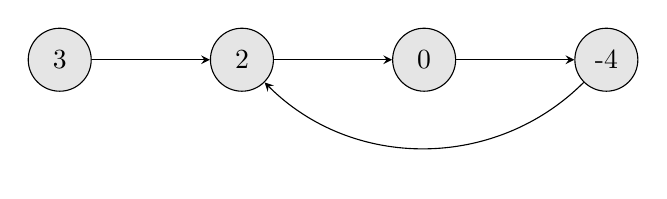
\begin{tikzpicture}
[mynode/.style={draw,circle,minimum size=8mm, fill=gray!20!}]
\node(){};
\node[mynode](3) {3};
\node[mynode](2)[right=15mm of 3] {2};
\node[mynode](0)[right=15mm of 2] {0};
\node[mynode](M4)[right=15mm of 0] {-4};
\draw[>=stealth,->] (3) -- (2);
\draw[>=stealth,->] (2) -- (0);
\draw[>=stealth,->] (0) -- (M4);
\draw[>=stealth,->] (M4) to[bend left=45] (2);
\end{tikzpicture}
\end{figure}
\textbf{Output}: \texttt{true}
\\
\textbf{Explanation}: There is a cycle in the linked list, where tail connects to the second node.
\end{flushleft}
\paragraph{Example 2:}
\begin{flushleft}
\textbf{Input}: $P=0$, $L$ is shown as below
\begin{figure}[H]
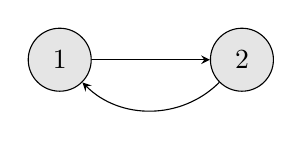
\begin{tikzpicture}
[mynode/.style={draw,circle,minimum size=8mm, fill=gray!20!}]
\node(){};
\node[mynode](1) {1};
\node[mynode](2)[right=15mm of 1] {2};
\draw[>=stealth,->] (1) -- (2);
\draw[>=stealth,->] (2) to[bend left=45] (1);
\end{tikzpicture}
\end{figure}
\textbf{Output}: \texttt{true}
\\
\textbf{Explanation}: There is a cycle in the linked list, where tail connects to the first node.
\end{flushleft}
\paragraph{Example 3:}
\begin{flushleft}
\textbf{Input}: $P=-1$, $L$ is
\begin{figure}[H]
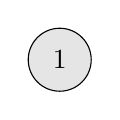
\begin{tikzpicture}
[mynode/.style={draw,circle,minimum size=8mm, fill=gray!20!}]
\node(){};
\node[mynode](1) {1};
\end{tikzpicture}
\end{figure}
\textbf{Output}: \texttt{false}
\\
\textbf{Explanation}: There is no cycle in the linked list.
\end{flushleft}
\paragraph{Follow up:}
\begin{itemize}
\item Can you solve it using $O(1)$ (i.e. constant) memory?
\end{itemize}
\subsection{Two Pointers}
Considering two pointers at different speed - a slow pointer and a fast pointer. The slow pointer moves one step at a time while the fast pointer moves two steps at a time.
\par
If there is no cycle in the list, the fast pointer will eventually reach the end and we can return \texttt{false} in this case.
\par
Now consider a cyclic list and imagine the slow and fast pointers are two runners racing around a circle track. The fast runner will eventually meet the slow runner. Why? Consider this case --- The fast runner is just one step behind the slow runner. In the next iteration, they both increment one and two steps respectively and meet each other.
\par
How about other cases? For example, we have not considered cases where the fast runner is two or three steps behind the slow runner yet. This is simple, because in the next or next's next iteration, this case will be reduced to case mentioned above.
\setcounter{algorithm}{0}
\begin{algorithm}[H]
\caption{Two Pointers}
\begin{algorithmic}[1]
\Procedure{HasCycle}{$H$}
\If{$H=\texttt{null}$}
\State \Return \texttt{false} \Comment Empty list
\EndIf
\State $F:=H$ \Comment The fast pointer
\State $S:=H$ \Comment The slow pointer
\While{$F\neq \texttt{null}$ \textbf{and} $F.\texttt{next}\neq \texttt{null}$}
\State $F\gets F.\texttt{next}$
\State $F\gets F.\texttt{next}$ \Comment $F$ move forward two steps
\State $S\gets S.\texttt{next}$ \Comment $S$ move forward one step
\If{$F=S$}
\State \Return \texttt{true}
\EndIf
\EndWhile
\State \Return \texttt{false}
\EndProcedure
\end{algorithmic}
\end{algorithm}
\section{142 --- Linked List Cycle II}
Given a linked list with head node $H$, return the node where the cycle begins. If there is no cycle, return \texttt{null}.
\par
To represent a cycle in the given linked list, we use an integer $P$ which represents the position (0-indexed) in the linked list where tail connects to. If $P$ is $-1$, then there is no cycle in the linked list.
\par
\textbf{Note}: Do not modify the linked list.
\paragraph{Example 1:}
\begin{flushleft}
\textbf{Input}:$P = 1$, $L$ is shown as below
\begin{figure}[H]
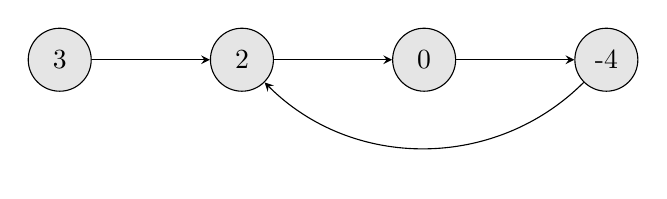
\begin{tikzpicture}
[mynode/.style={draw,circle,minimum size=8mm, fill=gray!20!}]
\node(){};
\node[mynode](3) {3};
\node[mynode](2)[right=15mm of 3] {2};
\node[mynode](0)[right=15mm of 2] {0};
\node[mynode](M4)[right=15mm of 0] {-4};
\draw[>=stealth,->] (3) -- (2);
\draw[>=stealth,->] (2) -- (0);
\draw[>=stealth,->] (0) -- (M4);
\draw[>=stealth,->] (M4) to[bend left=45] (2);
\end{tikzpicture}
\end{figure}
\textbf{Output}: tail connects to node index 1
\\
\textbf{Explanation}: There is a cycle in the linked list, where tail connects to the second node.
\end{flushleft}
\paragraph{Example 2:}
\begin{flushleft}
\textbf{Input}: $P=0$, $L$ is shown as below
\begin{figure}[H]
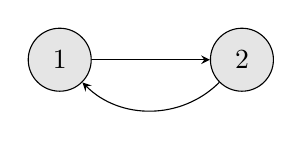
\begin{tikzpicture}
[mynode/.style={draw,circle,minimum size=8mm, fill=gray!20!}]
\node(){};
\node[mynode](1) {1};
\node[mynode](2)[right=15mm of 1] {2};
\draw[>=stealth,->] (1) -- (2);
\draw[>=stealth,->] (2) to[bend left=45] (1);
\end{tikzpicture}
\end{figure}
\textbf{Output}: tail connects to node index 0
\\
\textbf{Explanation}: There is a cycle in the linked list, where tail connects to the first node.
\end{flushleft}
\paragraph{Example 3:}
\begin{flushleft}
\textbf{Input}: $P=-1$, $L$ is
\begin{figure}[H]
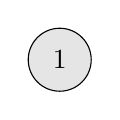
\begin{tikzpicture}
[mynode/.style={draw,circle,minimum size=8mm, fill=gray!20!}]
\node(){};
\node[mynode](1) {1};
\end{tikzpicture}
\end{figure}
\textbf{Output}: no cycle
\\
\textbf{Explanation}: There is no cycle in the linked list.
\end{flushleft}
\paragraph{Follow up:}
\begin{itemize}
\item Can you solve it without using extra space?
\end{itemize}
\subsection{Two Pointers}
首先还是用快慢指针确定是否是存在circle的linked list。如果是,则在两个指针相遇处,将另外一个指针重新指向list的header,然后两个指针每次都只前进一步,直至相遇,这时候的相遇处就是cycle begin的位置。

因为快指针每次走2,慢指针每次走1,快指针走的距离是慢指针的两倍。而快指针又比慢指针多走了一圈。所以 \fcj{head} 到loop的起点以及loop的起点到他们相遇的点的距离 与loop的长度相等。

当重新开始时,head移动到loop起点与相遇点到loop起点的距离也是相等的,相当于他们同时减掉了loop的起点到他们相遇的点的距离

\setcounter{lstlisting}{0}
\begin{lstlisting}[style=customc, caption={Two Pointers}]
ListNode *detectCycle( ListNode *head )
{
    //detect cycle
    auto slow = head;
    auto fast = head;
    while( fast && fast->next )
    {
        slow = slow->next;
        fast = fast->next->next;
        if( slow == fast )
        {
            break;
        }
    }
    //no cycle
    if( !fast || !fast->next )
    {
        return nullptr;
    }
    //find the meeting point
    slow = head;
    while( slow != fast )
    {
        slow = slow->next;
        fast = fast->next;
    }
    return fast;
}
\end{lstlisting}
\section{143 --- Reorder List}
Given a singly linked list $L$: 
\begin{figure}[H]
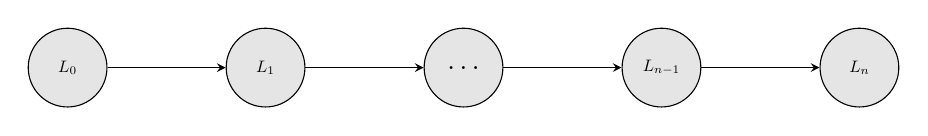
\begin{tikzpicture}
[mynode/.style={draw,circle,minimum size=10mm, fill=gray!20!}]
\node(){};
\node[mynode](0) {\scalebox{0.6}{$L_0$}};
\node[mynode](1)[right=15mm of 0] {\scalebox{0.6}{$L_1$}};
\node[mynode](2)[right=15mm of 1] {$\ldots$};
\node[mynode](n1)[right=15mm of 2] {\scalebox{0.6}{$L_{n-1}$}};
\node[mynode](n2)[right=15mm of n1] {\scalebox{0.6}{$L_n$}};
\draw[>=stealth,->] (0) -- (1);
\draw[>=stealth,->] (1) -- (2);
\draw[>=stealth,->] (2) -- (n1);
\draw[>=stealth,->] (n1) -- (n2);
\end{tikzpicture}
\end{figure}
reorder it to:
\begin{figure}[H]
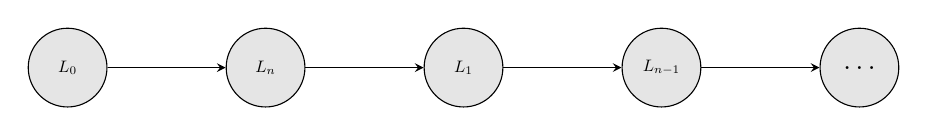
\begin{tikzpicture}
[mynode/.style={draw,circle,minimum size=10mm, fill=gray!20!}]
\node(){};
\node[mynode](0) {\scalebox{0.6}{$L_0$}};
\node[mynode](n2)[right=15mm of 0] {\scalebox{0.6}{$L_n$}};
\node[mynode](1)[right=15mm of n2] {\scalebox{0.6}{$L_1$}};
\node[mynode](n1)[right=15mm of 1] {\scalebox{0.6}{$L_{n-1}$}};
\node[mynode](2)[right=15mm of n1] {$\ldots$};
\draw[>=stealth,->] (0) -- (n2);
\draw[>=stealth,->] (n2) -- (1);
\draw[>=stealth,->] (1) -- (n1);
\draw[>=stealth,->] (n1) -- (2);
\end{tikzpicture}
\end{figure}
You may \textbf{not} modify the values in the list's nodes, only nodes itself may be changed.
\paragraph{Example 1:}
\begin{flushleft}
Given:
\begin{figure}[H]
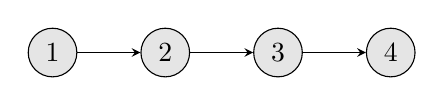
\begin{tikzpicture}
[mynode/.style={draw,circle,minimum size=5mm, fill=gray!20!}]
\node(){};
\node[mynode](1) {1};
\node[mynode](2)[right=8mm of 1] {2};
\node[mynode](3)[right=8mm of 2] {3};
\node[mynode](4)[right=8mm of 3] {4};
\draw[>=stealth,->] (1) -- (2);
\draw[>=stealth,->] (2) -- (3);
\draw[>=stealth,->] (3) -- (4);
\end{tikzpicture}
\end{figure}
Reorder to:
\begin{figure}[H]
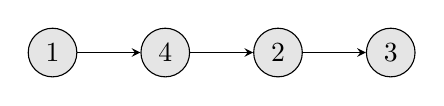
\begin{tikzpicture}
[mynode/.style={draw,circle,minimum size=5mm, fill=gray!20!}]
\node(){};
\node[mynode](1) {1};
\node[mynode](4)[right=8mm of 1] {4};
\node[mynode](2)[right=8mm of 4] {2};
\node[mynode](3)[right=8mm of 2] {3};
\draw[>=stealth,->] (1) -- (4);
\draw[>=stealth,->] (4) -- (2);
\draw[>=stealth,->] (2) -- (3);
\end{tikzpicture}
\end{figure}
\end{flushleft}
\paragraph{Example 2:}
\begin{flushleft}
Given:
\begin{figure}[H]
\begin{tikzpicture}
[mynode/.style={draw,circle,minimum size=5mm, fill=gray!20!}]
\node(){};
\node[mynode](1) {1};
\node[mynode](2)[right=8mm of 1] {2};
\node[mynode](3)[right=8mm of 2] {3};
\node[mynode](4)[right=8mm of 3] {4};
\node[mynode](5)[right=8mm of 4] {5};
\draw[>=stealth,->] (1) -- (2);
\draw[>=stealth,->] (2) -- (3);
\draw[>=stealth,->] (3) -- (4);
\draw[>=stealth,->] (4) -- (5);
\end{tikzpicture}
\end{figure}
Reorder to:
\begin{figure}[H]
\begin{tikzpicture}
[mynode/.style={draw,circle,minimum size=5mm, fill=gray!20!}]
\node(){};
\node[mynode](1) {1};
\node[mynode](5)[right=8mm of 1] {5};
\node[mynode](2)[right=8mm of 5] {2};
\node[mynode](4)[right=8mm of 2] {4};
\node[mynode](3)[right=8mm of 4] {3};
\draw[>=stealth,->] (1) -- (5);
\draw[>=stealth,->] (5) -- (2);
\draw[>=stealth,->] (2) -- (4);
\draw[>=stealth,->] (4) -- (3);
\end{tikzpicture}
\end{figure}
\end{flushleft}
\subsection{Two Pointers + Reverse}
首先用快慢指针找到链表的中间位置的node,然后从这个位置,将这个链表断开。然后对后半部分的链表进行reverse操作,最后合并两个链表。
\setcounter{lstlisting}{0}
\begin{lstlisting}[style=customc, caption={Two Pointers}]
void reorderList( ListNode* head )
{
    if( !head )
    {
        return;
    }
    //find middle node
    auto slow = head;
    auto fast = head;
    while( fast && fast->next )
    {
        slow = slow->next;
        fast = fast->next->next;
    }
    //right is the start of right half
    auto right = slow->next;
    //break left and right
    slow->next = nullptr;
    //reverse right half
    ListNode* pre = nullptr;
    auto cur = right;
    while( cur )
    {
        auto next = cur->next;
        cur->next = pre;
        pre = cur;
        cur = next;
    }
    //interleave with left and right
    auto left = head;
    right = pre;
    while( left && right )
    {
        //change left->next
        auto next = left->next;
        left->next = right;
        left = next;
        //change right->next
        next = right->next;
        right->next = left;
        right = next;
    }

}
\end{lstlisting}
\section{144 --- Binary Tree Preorder Traversal}
Given a binary tree with root node $R$, return the preorder traversal of its nodes' values.
\paragraph{Example:}
\begin{flushleft}
\textbf{Input}:
\begin{figure}[H]
\begin{tikzpicture}
[mynode/.style={draw,circle,minimum size=5mm, fill=gray!20!}]
\node(){};
\node[mynode](1) {1};
\node[mynode](2)[below=8mm of 1, xshift=8mm] {2};
\node[mynode](3)[below=8mm of 2, xshift=-8mm] {3};
\draw[>=stealth,->] (1) -- (2);
\draw[>=stealth,->] (2) -- (3);
\end{tikzpicture}
\end{figure}
\textbf{Output}: $[1,2,3]$
\end{flushleft}
\paragraph{Follow up:}
\begin{itemize}
\item Recursive solution is trivial, could you do it iteratively?
\end{itemize}
\subsection{Iterative With Stack}
How to traverse the tree
There are two general strategies to traverse a tree:
\begin{itemize}
    \item Breadth First Search (BFS): We scan through the tree level by level, following the order of height, from top to bottom. The nodes on higher level would be visited before the ones with lower levels.
    \item Depth First Search (DFS): In this strategy, we adopt the depth as the priority, so that one would start from a root and reach all the way down to certain leaf, and then back to root to reach another branch.
    \par
    The DFS strategy can further be distinguished as \textbf{preorder}, \textbf{inorder}, and \textbf{postorder} depending on the relative order among the root node, left node and right node.
\end{itemize}
In iterative approach, we simulate the recursive process, i.e., start from the root and then at each iteration pop the current node out of the stack and push its child nodes. In the implemented strategy we push nodes into output list following the order \fcj{top} $\rightarrow$ \fcj{bottom} and \fcj{left} $\rightarrow$ \fcj{right}, that naturally reproduces preorder traversal.

\setcounter{lstlisting}{0}
\begin{lstlisting}[style=customc, caption={Iterative Approach With Stack 1}]
vector<int> preorderTraversal( TreeNode* root )
{
    vector<int> ans;
    if( !root )
    {
        return ans;
    }
    stack<TreeNode*> stk;
    stk.push( root );
    while( !stk.empty() )
    {
        //visit current node first
        auto t = stk.top();
        stk.pop();
        ans.push_back( t->val );
        //add right node
        if( t->right )
        {
            stk.push( t->right );
        }
        //add left node
        if( t->left )
        {
            stk.push( t->left );
        }
    }
    return ans;
}
\end{lstlisting}

Another iterative approach uses a auxiliary node $p$ which is initialized as \fcj{root} at start. This approach can be seen as a template also for postorder and inorder traverse. 

In this approach, the \fcj{while} loop will check if the stack is empty or $p$ is a null node. If one condition is not met, then add non \fcj{null} node $p$ into the stack with adding the value of $p$ to the output. Then we change $p$ to its left child (when $p$ is a non \fcj{null} node). 

If $p$ is a \fcj{null} node, we get the top node $t$ from the stack and set $p$ to the right child of $t$.


\begin{lstlisting}[style=customc, caption={Iterative Approach With Stack 2}]
vector<int> preorderTraversal( TreeNode* root )
{
    vector<int> ans;
    if( !root )
    {
        return ans;
    }
    stack<TreeNode*> stk;
    auto p = root;
    while( !stk.empty() || p )
    {
        if( p )
        {
            //add current node to the stack
            //for future right child traverse
            stk.push( p );
            //we are in preorder
            //get p's value first
            ans.push_back( p->val );
            //change p to its left child
            p = p->left;
        }
        else
        {
            //p is a null node
            //get top node of the stack
            auto t = stk.top();
            stk.pop();
            //change p to its right child
            p = t->right;
        }
    }
    return ans;
}
\end{lstlisting}

\subsection{Morris Traversal}
The idea is to go down from the node to its predecessor $P$, and each predecessor $P$ will be visited twice. Suppose we are at node $T_0$, from this node we check if we can go left
\begin{itemize}
\item If the left child of $T_0$ exists, go right from the right child node of the left child until end. When we visit a leaf (node's predecessor) \textbf{1st time}, it has a zero right child, so we update output and establish the pseudo link \fcj{P.right=T0} to mark the fact the predecessor is visited. When we visit the same predecessor \textbf{the 2nd time}, it already points to $T_0$, thus we remove pseudo link and move right to the next node.
\item If the left child of $T_0$ is \fcj{null}, update output and move right to next node.
\end{itemize}
An example with detailed steps is shown as following:
\begin{figure}[H]
\begin{tikzpicture}
[mynode/.style={draw,circle,minimum size=5mm, fill=gray!20!}]
\node(){};
\node[mynode](1)[fill=red!20!] {1};
\node[mynode](2)[below=8mm of 1, xshift=-10mm] {2};
\node[mynode](5)[below=8mm of 1, xshift=10mm] {5};
\node[mynode](3)[below=8mm of 2, xshift=-8mm] {3};
\node[mynode](4)[below=8mm of 2, xshift=8mm] {4};
\draw[>=stealth,->] (1) -- (2);
\draw[>=stealth,->] (1) -- (5);
\draw[>=stealth,->] (2) -- (3);
\draw[>=stealth,->] (2) -- (4);
\end{tikzpicture}
\end{figure}
Starting from node 1. The status is: $T_0 = 1$. Is left child of $T_0$ \fcj{null}? No, then go left. 
\begin{figure}[H]
\begin{tikzpicture}
[mynode/.style={draw,circle,minimum size=5mm, fill=gray!20!}]
\node(){};
\node[mynode](1)[fill=red!20!] {1};
\node[mynode](2)[below=8mm of 1, xshift=-10mm, fill=blue!20!] {2};
\node[mynode](5)[below=8mm of 1, xshift=10mm] {5};
\node[mynode](3)[below=8mm of 2, xshift=-8mm] {3};
\node[mynode](4)[below=8mm of 2, xshift=8mm] {4};
\draw[>=stealth,->] (1) -- (2);
\draw[>=stealth,->] (1) -- (5);
\draw[>=stealth,->] (2) -- (3);
\draw[>=stealth,->] (2) -- (4);
\end{tikzpicture}
\end{figure}
Current Status: $T_0 = 1$, $P \gets 2$. Go right of $P$ until you meet \fcj{null} or current node $T_0$
\begin{figure}[H]
\begin{tikzpicture}
[mynode/.style={draw,circle,minimum size=5mm, fill=gray!20!}]
\node(){};
\node[mynode](1)[fill=red!20!] {1};
\node[mynode](2)[below=8mm of 1, xshift=-10mm, fill=blue!20!] {2};
\node[mynode](5)[below=8mm of 1, xshift=10mm] {5};
\node[mynode](3)[below=8mm of 2, xshift=-8mm] {3};
\node[mynode](4)[below=8mm of 2, xshift=8mm,fill=blue!20!] {4};
\draw[>=stealth,->] (1) -- (2);
\draw[>=stealth,->] (1) -- (5);
\draw[>=stealth,->] (2) -- (3);
\draw[>=stealth,->] (2) -- (4);
\end{tikzpicture}
\end{figure}
Current Status: $T_0 = 1$, $P \gets 4$, \fcj{P.right=null}. Now the right traverse reaches end, then
\begin{enumerate}
\item Add $T_0$'s value to the output
\item Link \fcj{P.right} to $T_0$, i.e., \fcj{4.right=1}.
\item Move $T_0$ to its left child, i.e. 2
\end{enumerate}
Now, output is $[1]$
\begin{figure}[H]
\begin{tikzpicture}
[mynode/.style={draw,circle,minimum size=5mm, fill=gray!20!}]
\node(){};
\node[mynode](1) {1};
\node[mynode](2)[below=8mm of 1, xshift=-10mm, fill=red!20!] {2};
\node[mynode](5)[below=8mm of 1, xshift=10mm] {5};
\node[mynode](3)[below=8mm of 2, xshift=-8mm] {3};
\node[mynode](4)[below=8mm of 2, xshift=8mm] {4};
\draw[>=stealth,->] (1) -- (2);
\draw[>=stealth,->] (1) -- (5);
\draw[>=stealth,->] (2) -- (3);
\draw[>=stealth,->] (2) -- (4);
\draw[>=stealth,->] (4) to[bend right=15] (1);
\end{tikzpicture}
\end{figure}
Current Status: $T_0 = 2$. Is left child of the node is \fcj{null}? No, then go left.
\begin{figure}[H]
\begin{tikzpicture}
[mynode/.style={draw,circle,minimum size=5mm, fill=gray!20!}]
\node(){};
\node[mynode](1) {1};
\node[mynode](2)[below=8mm of 1, xshift=-10mm, fill=red!20!] {2};
\node[mynode](5)[below=8mm of 1, xshift=10mm] {5};
\node[mynode](3)[below=8mm of 2, xshift=-8mm, fill=blue!20!] {3};
\node[mynode](4)[below=8mm of 2, xshift=8mm] {4};
\draw[>=stealth,->] (1) -- (2);
\draw[>=stealth,->] (1) -- (5);
\draw[>=stealth,->] (2) -- (3);
\draw[>=stealth,->] (2) -- (4);
\draw[>=stealth,->] (4) to[bend right=15] (1);
\end{tikzpicture}
\end{figure}
Current Status: $T_0 = 2$, $P = 3$. Go right of $P$ until you meet \fcj{null} or $T_0$. Since the right of 3 is \fcj{null}, then
\begin{enumerate}
\item Add $T_0$'s value to the output
\item Link \fcj{P.right=T0}, i.e., \fcj{3.right = 2}.
\item Move $T_0$ to its left child, i.e. 3
\end{enumerate}
Now, output is $[1,2]$
\begin{figure}[H]
\begin{tikzpicture}
[mynode/.style={draw,circle,minimum size=5mm, fill=gray!20!}]
\node(){};
\node[mynode](1) {1};
\node[mynode](2)[below=8mm of 1, xshift=-10mm] {2};
\node[mynode](5)[below=8mm of 1, xshift=10mm] {5};
\node[mynode](3)[below=8mm of 2, xshift=-8mm, fill=red!20!] {3};
\node[mynode](4)[below=8mm of 2, xshift=8mm] {4};
\draw[>=stealth,->] (1) -- (2);
\draw[>=stealth,->] (1) -- (5);
\draw[>=stealth,->] (2) -- (3);
\draw[>=stealth,->] (2) -- (4);
\draw[>=stealth,->] (4) to[bend right=15] (1);
\draw[>=stealth,->] (3) to[bend right=30] (2);
\end{tikzpicture}
\end{figure}
Current Status: $T_0 = 3$. Is left child of $T_0$ is \fcj{null}? Yes, then
\begin{enumerate}
\item Add $T_0$'s value to the output
\item Move to the right child of $T_0$, which is a 2.
\end{enumerate}
Now, output is $[1,2,3]$
\begin{figure}[H]
\begin{tikzpicture}
[mynode/.style={draw,circle,minimum size=5mm, fill=gray!20!}]
\node(){};
\node[mynode](1) {1};
\node[mynode](2)[below=8mm of 1, xshift=-10mm,fill=red!20!] {2};
\node[mynode](5)[below=8mm of 1, xshift=10mm] {5};
\node[mynode](3)[below=8mm of 2, xshift=-8mm] {3};
\node[mynode](4)[below=8mm of 2, xshift=8mm] {4};
\draw[>=stealth,->] (1) -- (2);
\draw[>=stealth,->] (1) -- (5);
\draw[>=stealth,->] (2) -- (3);
\draw[>=stealth,->] (2) -- (4);
\draw[>=stealth,->] (4) to[bend right=15] (1);
\draw[>=stealth,->] (3) to[bend right=30] (2);
\end{tikzpicture}
\end{figure}
Current Status: $T_0 = 2$. Is left child of $T_0$ is \fcj{null}? No, then go left. 
\begin{figure}[H]
\begin{tikzpicture}
[mynode/.style={draw,circle,minimum size=5mm, fill=gray!20!}]
\node(){};
\node[mynode](1) {1};
\node[mynode](2)[below=8mm of 1, xshift=-10mm,fill=red!20!] {2};
\node[mynode](5)[below=8mm of 1, xshift=10mm] {5};
\node[mynode](3)[below=8mm of 2, xshift=-8mm, fill=blue!20!] {3};
\node[mynode](4)[below=8mm of 2, xshift=8mm] {4};
\draw[>=stealth,->] (1) -- (2);
\draw[>=stealth,->] (1) -- (5);
\draw[>=stealth,->] (2) -- (3);
\draw[>=stealth,->] (2) -- (4);
\draw[>=stealth,->] (4) to[bend right=15] (1);
\draw[>=stealth,->] (3) to[bend right=30] (2);
\end{tikzpicture}
\end{figure}
Current Status: $T_0 = 2$, $P = 3$. Go right of $P$ until you meet \fcj{null} or $T_0$. Now, go right of 3 will meet 2, so
\begin{enumerate}
\item \textbf{Delete link} \fcj{P.right=T0}, i.e., \fcj{3.right=2}
\item Move to right child of $T_0$, i.e., 4.
\end{enumerate}
\begin{figure}[H]
\begin{tikzpicture}
[mynode/.style={draw,circle,minimum size=5mm, fill=gray!20!}]
\node(){};
\node[mynode](1) {1};
\node[mynode](2)[below=8mm of 1, xshift=-10mm] {2};
\node[mynode](5)[below=8mm of 1, xshift=10mm] {5};
\node[mynode](3)[below=8mm of 2, xshift=-8mm] {3};
\node[mynode](4)[below=8mm of 2, xshift=8mm, fill=red!20!] {4};
\draw[>=stealth,->] (1) -- (2);
\draw[>=stealth,->] (1) -- (5);
\draw[>=stealth,->] (2) -- (3);
\draw[>=stealth,->] (2) -- (4);
\draw[>=stealth,->] (4) to[bend right=15] (1);
\draw[>=stealth,->] (3) to[bend right=30] (2);
\end{tikzpicture}
\end{figure}
Current Status: $T_0 = 4$. Is left child of $T_0$ \fcj{null}? Yes, then
\begin{enumerate}
\item Add $T_0$'s value to output.
\item Move to the right child of $T_0$, which is 1.
\end{enumerate}
Now, output is $[1,2,3,4]$
\begin{figure}[H]
\begin{tikzpicture}
[mynode/.style={draw,circle,minimum size=5mm, fill=gray!20!}]
\node(){};
\node[mynode](1)[fill=red!20!] {1};
\node[mynode](2)[below=8mm of 1, xshift=-10mm] {2};
\node[mynode](5)[below=8mm of 1, xshift=10mm] {5};
\node[mynode](3)[below=8mm of 2, xshift=-8mm] {3};
\node[mynode](4)[below=8mm of 2, xshift=8mm] {4};
\draw[>=stealth,->] (1) -- (2);
\draw[>=stealth,->] (1) -- (5);
\draw[>=stealth,->] (2) -- (3);
\draw[>=stealth,->] (2) -- (4);
\draw[>=stealth,->] (4) to[bend right=15] (1);
\end{tikzpicture}
\end{figure}
Current Status: $T_0 = 1$. Is left child of $T_0$ is \fcj{null}? No, then go left. 
\begin{figure}[H]
\begin{tikzpicture}
[mynode/.style={draw,circle,minimum size=5mm, fill=gray!20!}]
\node(){};
\node[mynode](1)[fill=red!20!] {1};
\node[mynode](2)[below=8mm of 1, xshift=-10mm, fill=blue!20!] {2};
\node[mynode](5)[below=8mm of 1, xshift=10mm] {5};
\node[mynode](3)[below=8mm of 2, xshift=-8mm] {3};
\node[mynode](4)[below=8mm of 2, xshift=8mm] {4};
\draw[>=stealth,->] (1) -- (2);
\draw[>=stealth,->] (1) -- (5);
\draw[>=stealth,->] (2) -- (3);
\draw[>=stealth,->] (2) -- (4);
\draw[>=stealth,->] (4) to[bend right=15] (1);
\end{tikzpicture}
\end{figure}
Current Status: $T_0 = 1$, $P = 2$. Go right of $P$ until we meet \fcj{null} or $T_0$.
\begin{figure}[H]
\begin{tikzpicture}
[mynode/.style={draw,circle,minimum size=5mm, fill=gray!20!}]
\node(){};
\node[mynode](1)[fill=red!20!] {1};
\node[mynode](2)[below=8mm of 1, xshift=-10mm, fill=blue!20!] {2};
\node[mynode](5)[below=8mm of 1, xshift=10mm] {5};
\node[mynode](3)[below=8mm of 2, xshift=-8mm] {3};
\node[mynode](4)[below=8mm of 2, xshift=8mm, fill=blue!20!] {4};
\draw[>=stealth,->] (1) -- (2);
\draw[>=stealth,->] (1) -- (5);
\draw[>=stealth,->] (2) -- (3);
\draw[>=stealth,->] (2) -- (4);
\draw[>=stealth,->] (4) to[bend right=15] (1);
\end{tikzpicture}
\end{figure}
Current Status: $T_0 = 1$, $P = 4$, \fcj{P.right=T0}. We meet $T_0$, therefore
\begin{enumerate}
\item Delete link \fcj{P.right=T0}, (i.e. \fcj{4.right=1}).
\item Move to right child of $T_0$, i.e., 5.
\end{enumerate}
\begin{figure}[H]
\begin{tikzpicture}
[mynode/.style={draw,circle,minimum size=5mm, fill=gray!20!}]
\node(){};
\node[mynode]{1};
\node[mynode](2)[below=8mm of 1, xshift=-10mm] {2};
\node[mynode](5)[below=8mm of 1, xshift=10mm, fill=red!20!] {5};
\node[mynode](3)[below=8mm of 2, xshift=-8mm] {3};
\node[mynode](4)[below=8mm of 2, xshift=8mm] {4};
\draw[>=stealth,->] (1) -- (2);
\draw[>=stealth,->] (1) -- (5);
\draw[>=stealth,->] (2) -- (3);
\draw[>=stealth,->] (2) -- (4);
\end{tikzpicture}
\end{figure}
Current Status: $T_0 = 5$. Is left child of $T_0$ \fcj{null}? Yes, then
\begin{enumerate}
\item Add $T_0$'s value to output.
\item Move to right child of $T_0$
\end{enumerate}
Since we reach a \fcj{null} node, the whole process is finished.


\begin{lstlisting}[style=customc, caption={Morris Traversal}]
vector<int> preorderTraversal( TreeNode* root )
{
    vector<int> ans;
    auto node = root;
    while( node )
    {
        if( !node->left )
        {
            //no left child
            //we output current node's value
            ans.push_back( node->val );
            //and move to the right child
            node = node->right;
        }
        else
        {
            //we have to link the rightmost child of node
            //with it
            auto t = node->left;
            while( t->right && ( t->right != node ) )
            {
                t = t->right;
            }
            if( !t->right )
            {
                //first time to traverse node's child tree
                ans.push_back( node->val );
                t->right = node;
                //traverse node's left child
                node = node->left;
            }
            else
            {
                //second time to traverse node's child tree
                //this time left child tree has been visited
                //we first set t->right to null
                t->right = nullptr;
                //traverse node's right child
                node = node->right;
            }//end(t->right)
        }//end(node->left)
    }//end(while)

    return ans;
}
\end{lstlisting}
\section{145 --- Binary Tree Postorder Traversal}
Given a binary tree $R$, return the \textit{postorder} traversal of its nodes' values.
\paragraph{Example:}
\begin{flushleft}
\textbf{Input}:
\begin{figure}[H]
\begin{tikzpicture}
[mynode/.style={draw,circle,minimum size=5mm, fill=gray!20!}]
\node(){};
\node[mynode](1) {1};
\node[mynode](2)[below=8mm of 1, xshift=8mm] {2};
\node[mynode](3)[below=8mm of 2, xshift=-8mm] {3};
\draw[>=stealth,->] (1) -- (2);
\draw[>=stealth,->] (2) -- (3);
\end{tikzpicture}
\end{figure}
\textbf{Output}: $[3,2,1]$
\end{flushleft}
\paragraph{Follow up:}
\begin{itemize}
\item Recursive solution is trivial, could you do it iteratively?
\end{itemize}
\subsection{Stack}
和preorder一样,也有两种iterative的方法: stack和morris traversal。stack 的 output 过程和 preorder 类似,唯一不同的是需要先把left child放入stack中,另外最后要把得到的数组进行reverse。因为插入的过程中,当前节点的值都放在最前面了。

\setcounter{lstlisting}{0}
\begin{lstlisting}[style=customc, caption={Iteraive Apporach 1}]
vector<int> postorderTraversal( TreeNode* root )
{
    if( !root )
    {
        return {};
    }
    stack<TreeNode*> stk;
    stk.push( root );
    vector<int> ans;
    while( !stk.empty() )
    {
        auto t = stk.top();
        stk.pop();
        //we push left child first
        if( t->left )
        {
            stk.push( t->left );
        }
        //push right child second
        if( t->right )
        {
            stk.push( t->right );
        }
        //add current node's value
        ans.push_back( t->val );
    }
    //the sequence in the adding is root, right, left
    //thus after reverse, the sequence is left, right, root
    reverse( begin( ans ), end( ans ) );
    return ans;
}
\end{lstlisting}

The second approach using stack is with an auxiliary node $p$.

\begin{lstlisting}[style=customc, caption={Stack With Auxiliary Node}]
vector<int> postorderTraversal( TreeNode* root )
{
    if( !root )
    {
        return {};
    }
    stack<TreeNode*> stk;
    auto p = root;
    vector<int> ans;
    while( !stk.empty() || p )
    {
        if( p )
        {
            stk.push( p );
            //add current node's value to the output
            ans.push_back( p->val );
            //we visit right child tree first
            p = p->right;
        }
        else
        {
            auto t = stk.top();
            stk.pop();
            //visit left child tree
            p = t->left;
        }
    }
    //we need to reverse the output
    //since the sequence is root,right,left
    reverse( begin( ans ), end( ans ) );
    return ans;
}
\end{lstlisting} 

%\subsection{Morris Traversal}
%和Preorder方法类似,但是需要做改动,即,这时候需要看其right child是否存在,如果存在,则一直向左,然后建立link。如果不存在,则进入left child,并输出当前节点。
\section{146 --- LRU Cache}
Design and implement a data structure for \textcolor{red}{Least Recently Used (LRU)} cache. It should support the following operations: \fcj{get} and \fcj{put}.
\begin{itemize}
    \item \fcj{get(key)} --- Get the value (will always be positive) of the key if the key exists in the cache, otherwise return $-1$.
    \item \fcj{put(key, value)} --- Set or insert the value if the key is not already present. When the cache reached its capacity, it should invalidate the least recently used item before inserting a new item.
\end{itemize}
\paragraph{Example:}
\begin{flushleft}
\fcj{LRUCache cache = new LRUCache( 2 /* capacity */ );}

\fcj{cache.put(1, 1);}

\fcj{cache.put(2, 2);}

\fcj{cache.get(1);       // returns 1}

\fcj{cache.put(3, 3);    // evicts key 2}

\fcj{cache.get(2);       // returns -1 (not found)}

\fcj{cache.put(4, 4);    // evicts key 1}

\fcj{cache.get(1);       // returns -1 (not found)}

\fcj{cache.get(3);       // returns 3}

\fcj{cache.get(4);       // returns 4}


\end{flushleft}
\paragraph{Follow up:}
\begin{itemize}
    \item Could you do both operations in $O(1)$ time complexity?
\end{itemize}

\subsection{Hash Table Plus Double Linked List}
为了能够在$O(1)$的时间复杂度情况下,实现这两个函数,首先需要用一个hash table来建立key和value的映射。但是仅有这个还不够,为了能够在$O(1)$时间内获取LRU item,必须借助链表,将LRU item放置在链表队尾,而刚刚进行 \fcj{get} 和 \fcj{put} 操作的key则要放在链表的队头。
\begin{itemize}
    \item \fcj{get}: 首先看查询的key是否在hash table中,如果不存在,返回$-1$。否则,则把这个key和其对应的value从链表中删除,然后放置在链表的头位置。
    \item \fcj{put}: 首先看要放入的key是否在hash table中,
    \begin{enumerate}
        \item 如果存在,则同样把这个key和value组成的元素从链表中删除,然后放置在链表的头位置,然后退出。
        \item 反之,则将这个key和对应的value插入到hash table中,同时,在链表的头位置插入这对key和value组成的元素。同时检查是否超出允许的最大个数,如果超出了,将list队尾的key从hash table中删除,然后删除队尾元素。
    \end{enumerate}
\end{itemize}

\setcounter{lstlisting}{0}
\begin{lstlisting}[style=customc, caption={Hash Table With Linked List}]
class LRUCache
{
public:
    LRUCache( int capacity )
    {
        max_c = capacity;
    }
    int get( int key )
    {
        auto it = m.find( key );
        if( it == m.end() )
        {
            return -1;
        }
        //remove the (key,value) and put into the
        //begin of the list
        cache.splice( cache.begin(), cache, it->second );
        return it->second->second;
    }
    void put( int key, int value )
    {
        auto it = m.find( key );
        //this key exists
        if( it != m.end() )
        {
            //remove from the hash map
            //since the position in the list
            //is changed
            cache.erase( it->second );
        }
        //add (key,value) to the begin
        cache.emplace_front( key, value );
        m[key] = cache.begin();
        if( m.size() > max_c )
        {
            //remove the LRU
            int remove_key = cache.back().first;
            m.erase( remove_key );
            cache.pop_back();
        }
    }
    int max_c;
    list<pair<int, int>> cache;
    unordered_map<int, list<pair<int, int>>::iterator> m;
};
\end{lstlisting}

\section{147 --- Insertion Sort List}
Sort a linked list using insertion sort.  The partial sorted list initially contains only the first element in the list. With each iteration, one element is removed from the input data and inserted in-place into the sorted list
\par
Algorithm of Insertion Sort:
\begin{itemize}
    \item Insertion sort iterates, consuming one input element each repetition, and growing a sorted output list.
    \item At each iteration, insertion sort removes one element from the input data, finds the location it belongs within the sorted list, and inserts it there.
    \item It repeats until no input elements remain.
\end{itemize}
\paragraph{Example 1:}
\begin{flushleft}
\textbf{Input}:
\begin{figure}[H]
\begin{tikzpicture}
[mynode/.style={draw,circle,minimum size=8mm, fill=gray!20!}]
\node(){};
\node[mynode](1) {4};
\node[mynode](2)[right=12mm of 1] {2};
\node[mynode](3)[right=12mm of 2] {1};
\node[mynode](4)[right=12mm of 3] {3};
\draw[>=stealth,->] (1) -- (2);
\draw[>=stealth,->] (2) -- (3);
\draw[>=stealth,->] (3) -- (4);
\end{tikzpicture}
\end{figure}
\textbf{Output}: 
\begin{figure}[H]
\begin{tikzpicture}
[mynode/.style={draw,circle,minimum size=8mm, fill=gray!20!}]
\node(){};
\node[mynode](1) {1};
\node[mynode](2)[right=12mm of 1] {2};
\node[mynode](3)[right=12mm of 2] {3};
\node[mynode](4)[right=12mm of 3] {4};
\draw[>=stealth,->] (1) -- (2);
\draw[>=stealth,->] (2) -- (3);
\draw[>=stealth,->] (3) -- (4);
\end{tikzpicture}
\end{figure}
\end{flushleft}
\paragraph{Example 2:}
\begin{flushleft}
\textbf{Input}:
\begin{figure}[H]
\begin{tikzpicture}
[mynode/.style={draw,circle,minimum size=8mm, fill=gray!20!}]
\node(){};
\node[mynode](1) {$-1$};
\node[mynode](2)[right=12mm of 1] {5};
\node[mynode](3)[right=12mm of 2] {3};
\node[mynode](4)[right=12mm of 3] {4};
\node[mynode](5)[right=12mm of 4] {0};
\draw[>=stealth,->] (1) -- (2);
\draw[>=stealth,->] (2) -- (3);
\draw[>=stealth,->] (3) -- (4);
\draw[>=stealth,->] (4) -- (5);
\end{tikzpicture}
\end{figure}
\textbf{Output}: 
\begin{figure}[H]
\begin{tikzpicture}
[mynode/.style={draw,circle,minimum size=8mm, fill=gray!20!}]
\node(){};
\node[mynode](1) {$-1$};
\node[mynode](2)[right=12mm of 1] {0};
\node[mynode](3)[right=12mm of 2] {3};
\node[mynode](4)[right=12mm of 3] {4};
\node[mynode](5)[right=12mm of 4] {5};
\draw[>=stealth,->] (1) -- (2);
\draw[>=stealth,->] (2) -- (3);
\draw[>=stealth,->] (3) -- (4);
\draw[>=stealth,->] (4) -- (5);
\end{tikzpicture}
\end{figure}
\end{flushleft}
\subsection{Insertion Sort}
首先建立一个Dummy Header,这个dummy header将是排序后的链表的第一个节点。然后从当前链表的第一个节点开始,在每一次循环中,都在以dummy header开头的链表中寻找插入的位置。直至遍历完当前链表。最后返回dummy header的下一个节点作为排序后链表的头节点。

\setcounter{lstlisting}{0}
\begin{lstlisting}[style=customc, caption={Insertion Sort}]
public:
ListNode* insertionSortList( ListNode* head )
{
    //the list with dummy header
    //is the sorted list
    auto dummy = new ListNode( -1 );
    auto n = head;
    while( n )
    {
        //save next
        auto nxt = n->next;
        //in the list with dummy header
        //find the first node with value larger than
        //current node's value
        auto t = dummy;
        while( t->next && ( t->next->val <= n->val ) )
        {
            t = t->next;
        }
        //relink current node's next to t->next;
        n->next = t->next;
        //t either is dummy header or
        //a node with value no larger than n's value
        t->next = n;
        //move to the next node in the original node
        n = nxt;
    }
    auto ans = dummy->next;
    dummy->next = nullptr;
    return ans;
}
\end{lstlisting}
\section{148 --- Sort List}
Sort a linked list $H$ in $O(n\log_2 n)$ time using constant space complexity.
\paragraph{Example 1:}
\begin{flushleft}
\textbf{Input}:
\begin{figure}[H]
\begin{tikzpicture}
[mynode/.style={draw,circle,minimum size=8mm, fill=gray!20!}]
\node(){};
\node[mynode](1) {4};
\node[mynode](2)[right=12mm of 1] {2};
\node[mynode](3)[right=12mm of 2] {1};
\node[mynode](4)[right=12mm of 3] {3};
\draw[>=stealth,->] (1) -- (2);
\draw[>=stealth,->] (2) -- (3);
\draw[>=stealth,->] (3) -- (4);
\end{tikzpicture}
\end{figure}
\textbf{Output}: 
\begin{figure}[H]
\begin{tikzpicture}
[mynode/.style={draw,circle,minimum size=8mm, fill=gray!20!}]
\node(){};
\node[mynode](1) {1};
\node[mynode](2)[right=12mm of 1] {2};
\node[mynode](3)[right=12mm of 2] {3};
\node[mynode](4)[right=12mm of 3] {4};
\draw[>=stealth,->] (1) -- (2);
\draw[>=stealth,->] (2) -- (3);
\draw[>=stealth,->] (3) -- (4);
\end{tikzpicture}
\end{figure}
\end{flushleft}
\paragraph{Example 2:}
\begin{flushleft}
\textbf{Input}:
\begin{figure}[H]
\begin{tikzpicture}
[mynode/.style={draw,circle,minimum size=8mm, fill=gray!20!}]
\node(){};
\node[mynode](1) {$-1$};
\node[mynode](2)[right=12mm of 1] {5};
\node[mynode](3)[right=12mm of 2] {3};
\node[mynode](4)[right=12mm of 3] {4};
\node[mynode](5)[right=12mm of 4] {0};
\draw[>=stealth,->] (1) -- (2);
\draw[>=stealth,->] (2) -- (3);
\draw[>=stealth,->] (3) -- (4);
\draw[>=stealth,->] (4) -- (5);
\end{tikzpicture}
\end{figure}
\textbf{Output}: 
\begin{figure}[H]
\begin{tikzpicture}
[mynode/.style={draw,circle,minimum size=8mm, fill=gray!20!}]
\node(){};
\node[mynode](1) {$-1$};
\node[mynode](2)[right=12mm of 1] {0};
\node[mynode](3)[right=12mm of 2] {3};
\node[mynode](4)[right=12mm of 3] {4};
\node[mynode](5)[right=12mm of 4] {5};
\draw[>=stealth,->] (1) -- (2);
\draw[>=stealth,->] (2) -- (3);
\draw[>=stealth,->] (3) -- (4);
\draw[>=stealth,->] (4) -- (5);
\end{tikzpicture}
\end{figure}
\end{flushleft}
\subsection{Merge Sort}
由于链表的特性,Merge Sort是最适合的排序方法。首先把原链表分成左右两部分,分别对这两部分调用排序函数,然后将这两部分排序号的链表进行merge。

\setcounter{lstlisting}{0}
\begin{lstlisting}[style=customc, caption={Merge Sort}]
ListNode* sortList( ListNode* head )
{
    if( !head || !head->next )
    {
        return head;
    }
    auto slow = head;
    auto fast = head;
    auto pre = slow;
    //after the while loop
    //slow will be at the next of middle node
    //so we require a (pre) node to track the previous
    //node of slow
    //for example: 4->2->null, slow will be at 2.
    while( fast && fast->next )
    {
        pre = slow;
        slow = slow->next;
        fast = fast->next->next;
    }
    //break up the list
    pre->next = nullptr;
    //recursively sort left and right
    auto t1 = sortList( head );
    auto t2 = sortList( slow );
    //merge the result
    return merge( t1, t2 );
}
//merge routine
ListNode* merge( ListNode* l1, ListNode* l2 )
{
    auto dummy = new ListNode( -1 );
    auto merged = dummy;
    while( l1 && l2 )
    {
        if( l1->val <= l2->val )
        {
            merged->next = l1;
            l1 = l1->next;
        }
        else
        {
            merged->next = l2;
            l2 = l2->next;
        }

        merged = merged->next;
    }
    if( l1 )
    {
        merged->next = l1;
    }
    if( l2 )
    {
        merged->next = l2;
    }
    auto head = dummy->next;
    dummy->next = nullptr;
    delete dummy;
    return head;
}
\end{lstlisting}




\section{149 --- Max Points on a Line}
Given $n$ points on a 2D plane, find the maximum number of points that lie on the same straight line.
\section{150 --- Evaluate Reverse Polish Notation}
Evaluate the value of an arithmetic expression in Reverse Polish Notation.
\par
Valid operators are $+$, $-$, $\times$, $/$. Each operand may be an integer or another expression.
\paragraph{Note:}
\begin{itemize}
    \item Division between two integers should truncate toward zero.
    \item The given \texttt{RPN} expression is always valid. That means the expression would always evaluate to a result and there won't be any divide by zero operation.
\end{itemize}
\paragraph{Example 1:}
\begin{flushleft}
\textbf{Input}: $[2, 1, +, 3, \times]$
\\
\textbf{Output}: 9
\textbf{Explanation}: $((2 + 1) \times 3) = 9$
\end{flushleft}
\paragraph{Example 2:}
\begin{flushleft}
\textbf{Input}: $[4, 13, 5, /, +]$
\\
\textbf{Output}: 6
\\
\textbf{Explanation}: $(4 + (13 / 5)) = 6$
\end{flushleft}
\paragraph{Example 3:}
\begin{flushleft}
\textbf{Input}: $[10, 6, 9, 3, +, -11, \times, /, \times, 17, +, 5, +]$
\\
\textbf{Output}: 22
\\
\textbf{Explanation}:
\begin{align*}
& ((10 \times (6 / ((9 + 3) \times -11))) + 17) + 5 \\
&= ((10 \times (6 / (12 \times -11))) + 17) + 5 \\
&= ((10 \times (6 / -132)) + 17) + 5 \\
&= ((10 \times 0) + 17) + 5\\
&= (0 + 17) + 5\\
&= 17 + 5\\
&= 22\\
\end{align*}
\end{flushleft}
算法相对比较简单,用一个stack保存遇到的数字即数字运算的结果,步骤如下:
\begin{enumerate}
    \item 遍历字符串数组,遇到数字入栈
    \item 如果是操作符,则连续将栈顶的两个元素弹出,注意,对于减法和除法,第二个弹出的是左操作数,第一个弹出的是右操作数,将计算得到的结果压入栈中。
    \item 遍历完后,返回栈顶元素即为表达式结果。
\end{enumerate}
\setcounter{lstlisting}{0}
\begin{lstlisting}[style=customc, caption={Stack Based Approach}]
int evalRPN(vector<string>& tokens)
{
	stack<int> stk;
	
	for (const auto& s : tokens)
	{
		if (s[0] >= '0' && s[0] <= '9') // positive integers
		{
			int val = stoi(s);
			stk.push(val);
		}
		else if (s[0] == '-' && s.size() > 1) // negative integers with minus symbol
		{
			int val = stoi(s);
			stk.push(val);
		}
		else
		{
			int op1 = stk.top();
			stk.pop();
			int op2 = stk.top();
			stk.pop();

			switch (s[0])
			{
			case '+':
				stk.push(op1 + op2);
				break;

			case '-':
				stk.push(op2 - op1);
				break;

			case '/':
				stk.push(op2 / op1);
				break;

			case '*':
				stk.push(op1 * op2);
				break;
			}
		}
	}

	return stk.top();
}
\end{lstlisting}
%\section{151 --- Reverse Words in a String}
Given an input string $S$, reverse the string word by word.
\paragraph{Example:}
\begin{flushleft}
\textbf{Input}: \texttt{the sky is blue}
\\
\textbf{Output}: \texttt{blue is sky the}
\end{flushleft}
\paragraph{Note:}
\begin{itemize}
    \item A word is defined as a sequence of non-space characters.
    \item Input string may contain leading or trailing spaces. However, your reversed string should not contain leading or trailing spaces.
    \item You need to reduce multiple spaces between two words to a single space in the reversed string.
\end{itemize}
\paragraph{Follow up:}
\begin{itemize}
    \item For C programmers, try to solve it in-place in $O(1)$ space.
\end{itemize}    
\subsection{Two Pointers}
先整个字符串整体翻转一次,然后再分别翻转每一个单词(或者先分别翻转每一个单词,然后再整个字符串整体翻转一次),此时就能得到需要的结果了。这里采用双指针的方法或者双index的方法,假设$\alpha$是当前存储到的位置,$L$为字符串的长度。先reverse $S$,然后开始遍历$S$。遍历$S$用$\beta$,即当前访问的位置,遇到空格直接跳过,如果是非空格字符,这时候要判断$\alpha$是否为0,为0的话表示第一个单词,不用增加空格;如果不为0,说明不是第一个单词,需要在单词中间加一个空格,然后需要找到下一个单词的结束位置。这里用一个 \fcj{while} 循环来找下一个为空格的位置,在此过程中继续更新$\alpha$,相当于利用$S$的空间进行操作。找到单词的结束位置后,就reverse这个单词,然后更新$\beta$为结尾位置,最后遍历结束,最后把$\alpha$以后的部分去除掉就是最终的结果。
\setcounter{lstlisting}{0}
\begin{lstlisting}[style=customc, caption={Two Pointers}]
void reverseWords( string &s )
{
    //reverse the whole string first
    reverse( s.begin(), s.end() );
    size_t alpha = 0;
    for( size_t beta = 0; beta < s.size(); ++beta )
    {
        if( s[beta] != ' ' )
        {
            if( alpha != 0 )
            {
                //This is not the first word
                s[alpha] = ' ';
                ++alpha;
            }
            auto pos = beta;
            auto word_start = alpha;
            while( ( pos < s.size() ) && ( s[pos] != ' ' ) )
            {
                s[alpha] = s[pos];
                ++alpha;
                ++pos;
            }
            beta = pos;
            //alpha is at the next position of the last word,
            //therefore the reverse range is [word_start, alpha-1]
            reverse( s.begin() + word_start, s.begin() + alpha );
        }
    }
    s.resize( alpha );
}
\end{lstlisting}
%\section{152 --- Maximum Product Subarray}
Given an integer array $A$, find the contiguous subarray within an array (containing at least one number) which has the largest product.
\paragraph{Example 1:}
\begin{flushleft}
\textbf{Input}: \fcj{[2,3,-2,4]}

\textbf{Output}: 6

\textbf{Explanation}: \fcj{[2,3]} has the largest product 6.
\end{flushleft}

\paragraph{Example 2:}
\begin{flushleft}
\textbf{Input}: \fcj{[-2,0,-1]}

\textbf{Output}: 0

\textbf{Explanation}: The result cannot be 2, because \fcj{[-2,-1]} is not a subarray.
\end{flushleft}
\subsection{Kadane's Algorithm}
给予Kadane's algorithm,由于product受到正负数的影响,因此maintain两个变量:$x$和$y$,其中$x$是maximum subarray product ending at $i$,而$y$则是minimum subarray product ending at $i$。,同时用变量$P$代表目前为止所获得的最大product。遍历每一个数字时,首先确定当前数字$A[i]$,$x\times A[i]$和$y\times A[i]$三者中的最大值,由于这时候$x$会更新到这三者中的最大值,因此每次更新前将$x$保存到一个临时变量$z$中。然后确定数字$A[i]$, $z\times A[i]$和$y\times A[i]$三者中的最小值,将$y$更新为这个最小值。最后更新$P$为$P$和更新后的$x$两者中的最大值。遍历结束后,$P$即为所求最大product。
\setcounter{lstlisting}{0}
\begin{lstlisting}[style=customc, caption={Modified Kadane's Algorithm}]
int maxProduct( vector<int>& A )
{
	//x: max_ending_here
	int max_ending_here = A[0];
	//y: min_endign_here
	int min_ending_here = A[0];
	//P: max_so_far
	int max_so_far = A[0];

	for ( size_t i = 1; i < A.size(); ++i )
	{
		//save current alpha to a temp variable
		//z: cur_max
		int cur_max = max_ending_here;

		//update x
		max_ending_here = ( max )( A[i], min_ending_here * A[i] );
		max_ending_here = ( max )( max_ending_here, cur_max * A[i] );

		//update y
		min_ending_here = ( min )( A[i], min_ending_here * A[i] );
		min_ending_here = ( min )( min_ending_here, cur_max * A[i] );

		//update P
		max_so_far = ( max )( max_so_far, max_ending_here );
	}

	return max_so_far;
}
\end{lstlisting}
%\section{153 --- Find Minimum in Rotated Sorted Array}
Suppose an array $A$ sorted in ascending order is rotated at some pivot unknown to you beforehand. (i.e., $[0,1,2,4,5,6,7]$ might become  $[4,5,6,7,0,1,2]$).
\par
Find the minimum element.
\par
You may assume no duplicate exists in the array.
\paragraph{Example 1:}
\begin{flushleft}
\textbf{Input}: $[3,4,5,1,2]$
\\
\textbf{Output}: 1
\end{flushleft}
\paragraph{Example 2:}
\begin{flushleft}
\textbf{Input}: $[4,5,6,7,0,1,2]$
\\
\textbf{Output}: 0
\end{flushleft}
\subsection{Binary Search}
\begin{CJK*}{UTF8}{gbsn}
基于二分搜索,假设$l$, $r$是当前搜索的边界,那么位于中间位置$m=(l+r)/2$的数$A[m]$。如果这个数比$A[r]$大,那么表明最小值出现在$A[m+1\ldots r]$j区间内,如果比$A[r]$小,则最小值出现在$A[l\ldots m]$中。而题目中给出了没有重复的数字条件,因此不需要考虑$A[m]$和$A[r]$相等的情况。
\end{CJK*}
\setcounter{lstlisting}{0}
\begin{lstlisting}[style=customc, caption={Binary Search}]
int findMin( vector<int>& A )
{
	//right boundary of searching
	int r = static_cast< int >( A.size() - 1 ); 
	//left boundary of searching
	int l = 0;

	//We need l to be a valid index 
	//so the condition is (l < r)
	//not (l<=r)
	while ( l < r )
	{
		int mid = ( l + r ) / 2;

		if ( A[mid] > A[r] )
		{
			//The minimum is in [mid+1,r]
			l = mid + 1;
		}
		else
		{
			//The minimum is in [l, mid]
			r = mid;
		}
	}

	return A[l];
}
\end{lstlisting}

%\section{154 --- Find Minimum in Rotated Sorted Array II}
Suppose an array $A$ sorted in ascending order is rotated at some pivot unknown to you beforehand. (i.e.,  $[0,1,2,4,5,6,7]$ might become  $[4,5,6,7,0,1,2]$).
\par
Find the minimum element.
\par
The array may contain \textbf{duplicates}.
\paragraph{Example 1:}
\begin{flushleft}
\textbf{Input}: $[1,3,5]$
\\
\textbf{Output}: 1
\end{flushleft}
\paragraph{Example 2:}
\begin{flushleft}
\textbf{Input}: $[2,2,2,0,1]$
\\
\textbf{Output}: 0
\end{flushleft}
\paragraph{Note:}
\begin{itemize}
    \item This is a follow up problem to \textcolor{blue}{\textsc{Find Minimum in Rotated Sorted Array}}.
    \item Would allow duplicates affect the run-time complexity? How and why?
\end{itemize}
\subsection{Binary Search}
\begin{CJK*}{UTF8}{gbsn}
这里和153基本类似,不过这里允许重复数字存在。因此算法和153基本类似,唯一不同的是,当$A[m]=A[r]$时,需要将$r$往左移动一个位置,然后继续进行比较。由于重复元素的存在,当然$A[m]=A[r]$时,实际上就成了线性搜索,特别的,当$A$中所有数字都相等时,时间复杂度就是$O(n)$。
\end{CJK*}
\setcounter{lstlisting}{0}
\begin{lstlisting}[style=customc, caption={Binary Search}]
int findMin( vector<int>& A )
{
	//right boundry of searching
	int r = static_cast< int >( A.size() - 1 ); 
	//left boundry of searching
	int l = 0;

	//We need l to be a valid index 
	//so the condition is (l < r)
	//not (l<=r)
	while ( l < r )
	{
		int mid = ( l + r ) / 2;

		if ( A[mid] > A[r] )
		{
			//The minimum is in [mid+1,r]
			l = mid + 1;
		}
		else if( A[mid] < A[r] )
		{
			//The minimum is in [l, mid]
			r = mid;
		}
		else  // A[m]=A[r]
		{
			//Left move r by one index
			--r;
		}
	}

	return A[l];
}
\end{lstlisting}
%\section{155 --- Min Stack}
Design a stack that supports \texttt{push}, \texttt{pop}, \texttt{top}, and retrieving the minimum element in constant time.
\begin{itemize}
\item \fcj{push(x)} --- Push element x onto stack.
\item \fcj{pop()} --- Removes the element on top of the stack.
\item \fcj{top()} --- Get the top element.
\item \fcj{getMin()} --- Retrieve the minimum element in the stack.
\end{itemize}
\paragraph{Example:}
\begin{flushleft}


\fcj{MinStack minStack = new MinStack();}

\fcj{minStack.push(-2);}

\fcj{minStack.push(0);}

\fcj{minStack.push(-3);}

\fcc{minStack.getMin();   // Returns -3.}

\fcj{minStack.pop();}

\fcj{minStack.top();      // Returns 0.}

\fcj{minStack.getMin();   // Returns -2.}
\end{flushleft}

\subsection{One Stack}

这里涉及到如何利用stack的特性的技巧,为了得到stack中的最小值,同时又能保证弹出操作能够正确的更新最小值,可以将当前最小值和要压入的值一起放入stack中,一种做法是先放入当前值,在放入当前最小值,这样栈顶就是最小值。这样,当弹出时,需要弹出两个。然后如果栈不为空,就用栈顶元素更新最小值。

而对于\fcj{top()},由于栈顶元素是最小值,因此需要先把当前栈顶元素弹出,然后获得剩下的栈的栈顶元素,再把弹出的最小值重新压入栈中。

\setcounter{lstlisting}{0}
\begin{lstlisting}[style=customc, caption={Push Two Values At Same Time}]
class MinStack
{
public:
	/** initialize your data structure here. */
	MinStack ()
	{
		m_min = -1;
	}

	void push ( int x )
	{
		if( m_stk.empty () )
		{
			//This is the first time
			//to push into stack
			m_min = x;
		}
		else
		{
			//Update current minimum value
			m_min = ( min ) ( x, m_min );
		}

		//Push x first
		m_stk.push ( x );
		//Push current minimum value
		m_stk.push ( m_min );
	}

	void pop ()
	{
		if( !m_stk.empty () )
		{
			//Pop minimum value
			m_stk.pop ();
			//Pop actual value
			m_stk.pop ();

			if( !m_stk.empty () )
			{
				//Update current minimum value
				m_min = m_stk.top ();
			}
		}
	}

	int top ()
	{
		//we have to pop current top first
		//because it is m_min
		m_stk.pop ();
		//This is the actual top
		int x = m_stk.top ();
		//Push m_min to stack again
		m_stk.push ( m_min );
		return x;
	}

	int getMin ()
	{
		return m_min;
	}

	// The minimum value in the stack
	int m_min;
	// The stack
	stack<int> m_stk;
};
\end{lstlisting}

\subsection{Two Stacks}
We can use two stacks: one is used to store numbers and the other to store minimum number so far.

\begin{lstlisting}[style=customc, caption={Two Stacks}]
class MinStack
{
public:
    /** initialize your data structure here. */
    MinStack() {}
    void push( int x )
    {
        stk.push( x );
        if( aux.empty() )
        {
            aux.push( x );
        }
        else
        {
            int t = aux.top();
            //add minimum number so far
            aux.push( ( min )( x, t ) );
        }
    }
    void pop()
    {
        if( stk.empty() )
        {
            return;
        }
        stk.pop();
        aux.pop();
    }
    int top()
    {
        return stk.top();
    }
    int getMin()
    {
        return aux.top();
    }
    stack<int> stk;
    stack<int> aux;
};
\end{lstlisting}
%\section{156 --- Binary Tree Upside Down}
Given a binary tree with root $R$, where all the right nodes are either leaf nodes with a sibling (a left node that shares the same parent node) or empty, flip it upside down and turn it into a tree where the original right nodes turned into left leaf nodes. Return the new root.
\paragraph{For example:}
\begin{flushleft}
Given a binary tree
\begin{figure}[H]
\begin{tikzpicture}
[mynode/.style={draw,circle,minimum size=5mm, fill=gray!20!}]
\node(){};
\node[mynode](1) {1};
\node[mynode](2)[below=8mm of 1, xshift=-8mm] {2};
\node[mynode](3)[below=8mm of 1, xshift=8mm] {3};
\node[mynode](4)[below=8mm of 2, xshift=-8mm] {4};
\node[mynode](5)[below=8mm of 2, xshift=8mm] {5};
\draw[>=stealth,->] (1) -- (2);
\draw[>=stealth,->] (1) -- (3);
\draw[>=stealth,->] (2) -- (4);
\draw[>=stealth,->] (2) -- (5);
\end{tikzpicture}
\end{figure}
return the root of the binary tree
\begin{figure}[H]
\begin{tikzpicture}
[mynode/.style={draw,circle,minimum size=5mm, fill=gray!20!}]
\node(){};
\node[mynode](1) {4};
\node[mynode](2)[below=8mm of 1, xshift=-8mm] {5};
\node[mynode](3)[below=8mm of 1, xshift=8mm] {2};
\node[mynode](4)[below=8mm of 3, xshift=-8mm] {3};
\node[mynode](5)[below=8mm of 3, xshift=8mm] {1};
\draw[>=stealth,->] (1) -- (2);
\draw[>=stealth,->] (1) -- (3);
\draw[>=stealth,->] (3) -- (4);
\draw[>=stealth,->] (3) -- (5);
\end{tikzpicture}
\end{figure}
\end{flushleft}
\subsection{Recursive Approach}

对于一个根节点来说,目标是将其左子节点变为根节点,右子节点变为左子节点,原来的根节点变为右子节点,那么我们判断这个root是否存在,且其有没有left child node,如果不满足这两个条件的话,直接返回即可,否则对left child node调用递归函数,直到到达most left开始翻转,翻转好most left child node后,开始回到上一个left child node继续翻转即可,直至翻转完The whole tree。

另外注意到题目中给出的特性,所有的右节点要么没有,要么就是叶子节点并且一定有个兄弟节点。

%\setcounter{algorithm}{0}
%\begin{algorithm}[H]
%\caption{Recursive Approach}
%\begin{algorithmic}[1]
%\Procedure{UpsideDownBinaryTree}{$R$}
%\If{$R=\texttt{null}$ \textbf{or} $R.\texttt{left}=\texttt{null}$}
%\State \Return $R$ \Comment root or left child is empty
%\EndIf
%\State $l:=R.\texttt{left}$ \Comment The left child node of current root $R$
%\State $r:=R.\texttt{right}$ \Comment The right child node of current root $R$
%\State $\hat{R}:=\texttt{UpsideDownBinaryTree}(l)$ \Comment Recursively operating on left tree
%\State $l.\texttt{left}\gets r$ \Comment Change left child node of $l$ to $r$
%\State $l.\texttt{right}\gets R$ \Comment Change right child node $l$ to $R$
%\State $R.\texttt{left}\gets\texttt{null}$ \Comment Set left and right child nodes of current root $R$ to empty
%\State $R.\texttt{right}\gets\texttt{null}$
%\State \Return $\hat{R}$
%\EndProcedure
%\end{algorithmic}
%\end{algorithm}
\setcounter{lstlisting}{0}
\begin{lstlisting}[style=customc, caption={Recursive Approach}]
TreeNode *upsideDownBinaryTree( TreeNode *root )
{
    if( !root || !root->left )
    {
        return root;
    }
    //save left child node
    auto l = root->left;
    //save right child node
    auto r = root->right;
    //Recursive call the function to get the
    //root of upside-down left child tree
    auto ans = upsideDownBinaryTree( l );
    //left's left child node is its parent's right child: right
    l->left = r;
    //left's right child node is its parent: root
    l->right = root;
    //root become leaf
    root->left = nullptr;
    root->right = nullptr;
    //This is the new root of the changed tree
    return ans;
}
\end{lstlisting}

\subsection{Iterative}
In this approach, we visit each left child node and change its left and child node. More specifically, suppose we are visiting a node $t$ and its parent node is $p$

\begin{enumerate}
\item Change \fcj{t->left} to \fcj{p->right}.
\item Change \fcj{t->right} to \fcj{p}.
\end{enumerate}

Thus, we need to save current node and its right node before moving to current node's left child.


\begin{lstlisting}[style=customc, caption={Iterative}]
TreeNode* upsideDownBinaryTree( TreeNode* root )
{
    //save right child of last visited node
    TreeNode* x = nullptr;
    //save last visited node
    TreeNode* y = nullptr;
    auto node = root;
    while( node )
    {
        //save left child as next
        //for successive visit
        auto next = node->left;
        //change left child to the right child of its parent
        //i.e. the sibling: x
        node->left = x;
        //save its right child to x
        x = node->right;
        //change right child to its parent: y
        node->right = y;
        //save node to y
        y = node;
        //move to its previous left child
        node = next;
    }
    //now y is the new root
    return y;
}
\end{lstlisting}

%\section{157 --- Read N Characters Given Read4}
Given a file and assume that you can only read the file using a given method \fcj{read4}, implement a method to read $n$ characters.
 

\paragraph{Method read4:}

\begin{flushleft}
The API \fcj{read4} reads 4 consecutive characters from the file, then writes those characters into the buffer array \fcj{buf}.

The return value is the number of actual characters read.

Note that \fcj{read4()} has its own file pointer, much like \fcj{FILE *fp} in C.

Definition of \fcj{read4}: \fcj{int read4(char[] buf)}
\end{flushleft}

\paragraph{Note:} 

\begin{itemize}
\item \fcj{buf[]} is destination not source, the results from \fcj{read4} will be copied to \fcj{buf[]}
\end{itemize}

Below is a high level example of how read4 works:

\begin{flushleft}
\fcj{File file("abcdefghijk"); // initially file pointer (fp) points to 'a'}

\fcj{char[] buf = new char[4]; // Create buffer with enough space to store characters}

\fcj{read4(buf); // read4 returns 4. Now buf = "abcd", fp points to 'e'}

\fcj{read4(buf); // read4 returns 4. Now buf = "efgh", fp points to 'i'}

\fcj{read4(buf); // read4 returns 3. Now buf = "ijk", fp points to end of file}
\end{flushleft}
 
\paragraph{Method read:}

\begin{flushleft}
By using the \fcj{read4} method, implement the method \fcj{read} that reads $n$ characters from the file and store it in the buffer array \fcj{buf}. Consider that you \textbf{cannot} manipulate the file directly.

The return value is the number of actual characters read.

Definition of \fcj{read}: \fcj{int read(char[] buf, int n)}
\end{flushleft}

\paragraph{Note:} 

\begin{itemize}
\item \fcj{buf[]} is destination not source, you will need to write the results to \fcj{buf[]}.
\end{itemize}
 

\paragraph{Example 1:}

\begin{flushleft}
\textbf{Input}: \fcj{file = "abc"}, $n = 4$

\textbf{Output}: 3

\textbf{Explanation}: 

After calling your \fcj{read} method, \fcj{buf} should contain \fcj{"abc"}. We read a total of 3 characters from the file, so return 3. Note that \fcj{"abc"} is the file's content, not \fcj{buf}. \fcj{buf} is the destination buffer that you will have to write the results to.

\end{flushleft}
\paragraph{Example 2:}

\begin{flushleft}
\textbf{Input}: \fcj{file = "abcde"}, $n = 5$

\textbf{Output}: 5

\textbf{Explanation}: 

After calling your \fcj{read} method, buf should contain \fcj{"abcde"}. We read a total of 5 characters from the file, so return 5.

\end{flushleft}

\paragraph{Example 3:}

\begin{flushleft}
\textbf{Input}: \fcj{file = "abcdABCD1234"}, $n = 12$

\textbf{Output}: 12

\textbf{Explanation}: After calling your read method, \fcj{buf} should contain \fcj{"abcdABCD1234"}. We read a total of 12 characters from the file, so return 12.
\end{flushleft}

\paragraph{Example 4:}

\begin{flushleft}
\textbf{Input}: \fcj{file = "leetcode"}, $n = 5$

\textbf{Output}: 5

\textbf{Explanation}: After calling your read method, \fcj{buf} should contain \fcj{"leetc"}. We read a total of 5 characters from the file, so return 5.
\end{flushleft}
 

\paragraph{Note:}

\begin{itemize}
\item Consider that you cannot manipulate the file directly, the file is only accessible for \fcj{read4} but not for \fcj{read}.
\item The \fcj{read} function will only be called once for each test case.
\item You may assume the destination buffer array, \fcj{buf}, is guaranteed to have enough space for storing $n$ characters.
\end{itemize}
\subsection{Analysis}

比较简单的题目,每次调用\fcj{read4},直到返回值变为零,表示已经全部读完。另外每次调用\fcj{read4}的时候,将\fcj{p}指针根据返回值调整到下一个开始读取的位置。

%\setcounter{algorithm}{0}
%\begin{algorithm}[H]
%\caption{Implementation read By read4}
%\begin{algorithmic}[1]
%\Procedure{Read}{$p, n$}
%\State $x:=0$ \Comment The read result of each calling \texttt{read4}
%\While{$\texttt{true}$}
%\State $y:= \texttt{read4(p+x)}$ \Comment $y$ is the count of characters read from the file
%\If{$y = 0$}
%\State \texttt{break} \Comment Finished reading from the file
%\EndIf
%\State $x\gets x+y$ \Comment Update current total counts of characters 
%\EndWhile
%\State \Return $\min(x, n)$ \Comment The file may contain less than $n$ characters
%\EndProcedure
%\end{algorithmic}
%\end{algorithm}

\setcounter{lstlisting}{0}
\begin{lstlisting}[style=customc, caption={Pointer}]
// Forward declaration of the read4 API.
int read4( char *buf );
/**
 * @param buf Destination buffer
 * @param n   Number of characters to read
 * @return    The number of actual characters read
 */
int read( char *buf, int n )
{
    int total = 0;
    while( total < n )
    {
        int x = read4( buf );
        if( x == 0 )
        {
            //no content
            break;
        }
        //add to total
        total += x;
        //move the buffer pointer
        buf += x;
    }
    //total may be large than n
    //we return the minimum of total and n
    return ( min )( total, n );
}
\end{lstlisting}
%\section{158 --- Read N Characters Given Read4 II - Call multiple times }
The API: \texttt{int read4(char *buf)} reads 4 characters at a time from a file.
\par
The return value is the actual number of characters read.
\par
For example, it returns 3 if there is only 3 characters left in the file.
\par
By using the read4 API, implement the function \texttt{int read(char *p, int n)} that reads $n$ characters from the file.
\paragraph{Note:}
\begin{itemize}
\item The \texttt{read} function may be called \texttt{multiple} times..
\end{itemize}
\subsection{Analysis}
\begin{CJK*}{UTF8}{gbsn}
这道题是之前157 --- \textbf{Read N Characters Given Read4}的拓展,不同点在于这里\texttt{read}函数可以调用多次,那么难度就增加了,例如:要读取的文件buffer为\texttt{ab},然后执行read(1),read(2),那么第一次调用\texttt{read(1)}后,从buffer中读出一个字符,那么就是第一个字符\texttt{a},然后又调用了一个\texttt{read(2)},但是buffer中只剩一个\texttt{b}了,所以就把取出的结果就是\texttt{b}。
\par
另外一个例子更能说明不同: 文件的buffer为\texttt{a}, 分别执行\texttt{read(0)},\texttt{read(1)},\texttt{read(2)}。第一次调用read(0),不会读取任何字符。第二次调用\texttt{read(1)},取一个字符,而buffer中只有一个字符\texttt{a},因此返回\texttt{a}。然后调用read(2),但是这时候buffer中没有字符了,所以同样不会读取任何字符。
\end{CJK*}
%\section{159 --- Longest Substring with At Most Two Distinct Characters}
Given a string $S$, find the length of the longest substring $T$ that contains at most two distinct characters.
\par
\paragraph{Example:}
\begin{flushleft}
\textbf{Input}: $S = \texttt{eceba}$
\\
\textbf{Output}: $T=\texttt{ece}$ and its length is 3.
\end{flushleft}
%\section{160 --- Intersection of Two Linked Lists}
Write a program to find the node at which the intersection of two singly linked lists begins.
\par
For example, the following two linked lists:
\begin{figure}[H]
\begin{tikzpicture}
[mynode/.style={draw,circle,minimum size=1cm, fill=gray!20!}]
\node(){};
\node[minimum size=1cm](A) {A:};
\node[minimum size=1cm](E)[right=8mm of A] {};
\node[mynode](a1)[right=8mm of E] {$a_1$};
\node[mynode](a2)[right=8mm of a1] {$a_2$};
\node[minimum size=1cm](B) [below=1.6cm of A]{B:};
\node[mynode](b1)[right=8mm of B] {$b_1$};
\node[mynode](b2)[right=8mm of b1] {$b_2$};
\node[mynode](b3)[right=8mm of b2] {$b_3$};
\node[mynode](c1)[right=8mm of b3, yshift=1.2cm] {$c_1$};
\node[mynode](c2)[right=8mm of c1] {$c_2$};
\node[mynode](c3)[right=8mm of c2] {$c_3$};
\draw[>=stealth,->] (a1) -- (a2);
\draw[>=stealth,->] (a2) to[bend left=15] (c1);
\draw[>=stealth,->] (b1) -- (b2);
\draw[>=stealth,->] (b2) -- (b3);
\draw[>=stealth,->] (b3) to[bend right=15] (c1);
\draw[>=stealth,->] (a2) to[bend left=15] (c1);
\draw[>=stealth,->] (c1) -- (c2);
\draw[>=stealth,->] (c2) -- (c3);
\end{tikzpicture}
\end{figure}

begin to intersect at node $c_1$.
\paragraph{Example 1:}
\begin{flushleft}
\textbf{Input}:
\\
\begin{figure}[H]
\begin{tikzpicture}
[mynode/.style={draw,circle,minimum size=1cm, fill=gray!20!}]
\node(){};
\node[minimum size=1cm](A) {A:};
\node[minimum size=1cm](E)[right=8mm of A] {};
\node[mynode](a1)[right=8mm of E] {4};
\node[mynode](a2)[right=8mm of a1] {1};
\node[minimum size=1cm](B) [below=1.6cm of A]{B:};
\node[mynode](b1)[right=8mm of B] {5};
\node[mynode](b2)[right=8mm of b1] {0};
\node[mynode](b3)[right=8mm of b2] {1};
\node[mynode](c1)[right=8mm of b3, yshift=1.2cm] {8};
\node[mynode](c2)[right=8mm of c1] {4};
\node[mynode](c3)[right=8mm of c2] {5};
\draw[>=stealth,->] (a1) -- (a2);
\draw[>=stealth,->] (a2) to[bend left=15] (c1);
\draw[>=stealth,->] (b1) -- (b2);
\draw[>=stealth,->] (b2) -- (b3);
\draw[>=stealth,->] (b3) to[bend right=15] (c1);
\draw[>=stealth,->] (a2) to[bend left=15] (c1);
\draw[>=stealth,->] (c1) -- (c2);
\draw[>=stealth,->] (c2) -- (c3);
\end{tikzpicture}
\end{figure}
\textbf{Output}: Reference of the node with value $= 8$
\\
\textbf{Input Explanation}: The intersected node's value is 8 (note that this must not be 0 if the two lists intersect). From the head of $A$, it reads as $[4,1,8,4,5]$. From the head of $B$, it reads as $[5,0,1,8,4,5]$. There are 2 nodes before the intersected node in $A$; There are 3 nodes before the intersected node in $B$.
\end{flushleft}

\paragraph{Example 2:}
\begin{flushleft}
\textbf{Input}:
\begin{figure}[H]
\begin{tikzpicture}
[mynode/.style={draw,circle,minimum size=1cm, fill=gray!20!}]
\node(){};
\node[minimum size=1cm](A) {A:};
\node[mynode](a1)[right=8mm of A] {0};
\node[mynode](a2)[right=8mm of a1] {9};
\node[mynode](a3)[right=8mm of a2] {1};
\node[minimum size=1cm](B) [below=1.6cm of A]{B:};
\node[minimum size=1cm](E1)[right=8mm of B] {};
\node[minimum size=1cm](E2)[right=8mm of E1] {};
\node[mynode](b1)[right=8mm of E2] {3};
\node[mynode](c1)[right=8mm of b3, yshift=1.2cm] {2};
\node[mynode](c2)[right=8mm of c1] {4};
\draw[>=stealth,->] (a1) -- (a2);
\draw[>=stealth,->] (a2) -- (a3);
\draw[>=stealth,->] (a3) to[bend left=15] (c1);
\draw[>=stealth,->] (b1) to[bend right=15] (c1);
\draw[>=stealth,->] (c1) -- (c2);
\end{tikzpicture}
\end{figure}
\textbf{Output}: Reference of the node with value $= 2$
\\
\textbf{Input Explanation}: The intersected node's value is 2 (note that this must not be 0 if the two lists intersect). From the head of $A$, it reads as $[0,9,1,2,4]$. From the head of $B$, it reads as $[3,2,4]$. There are 3 nodes before the intersected node in $A$; There are 1 node before the intersected node in $B$.
\end{flushleft}

\paragraph{Example 3:}
\begin{flushleft}
\textbf{Input}:
\\
\begin{figure}[H]
\begin{tikzpicture}
[mynode/.style={draw,circle,minimum size=1cm, fill=gray!20!}]
\node(){};
\node[minimum size=1cm](A) {A:};
\node[mynode](a1)[right=8mm of A] {2};
\node[mynode](a2)[right=8mm of a1] {6};
\node[mynode](a3)[right=8mm of a2] {4};
\node[minimum size=1cm](B) [below=1.6cm of A]{B:};
\node[minimum size=1cm](E)[right=8mm of B] {};
\node[mynode](b1)[right=8mm of E] {1};
\node[mynode](b2)[right=8mm of b1] {5};
\draw[>=stealth,->] (a1) -- (a2);
\draw[>=stealth,->] (a2) -- (a3);
\draw[>=stealth,->] (b1) -- (b2);
\end{tikzpicture}
\end{figure}
\textbf{Output}: Reference of the node with value $= 8$
\\
\textbf{Input Explanation}: From the head of $A$, it reads as $[2,6,4]$. From the head of $B$, it reads as $[1,5]$. Since the two lists do not intersect, intersectVal must be 0
\\.
\textbf{Explanation}: The two lists do not intersect, so return \texttt{null}.
\end{flushleft}
\paragraph{Notes:}
\begin{itemize}
\item If the two linked lists have no intersection at all, return \texttt{null}.
\item The linked lists must retain their original structure after the function returns.
\item You may assume there are no cycles anywhere in the entire linked structure.
\item Your code should preferably run in $O(n)$ time and use only $O(1)$ memory.
\end{itemize}
\subsection{Two Pointers}
\begin{itemize}
\item Maintain two pointers $x$ and $y$ initialized at the head of $A$ and $B$, respectively. Then let them both traverse through the lists, one node at a time.
\item When $x$ reaches the end of a list, then redirect it to the head of $B$; similarly when $y$ reaches the end of a list, redirect it the head of $A$.
\item If at any point $x$ meets $y$, then $x/y$ is the intersection node.
\item If two lists have intersection, then their last nodes must be the same one. So when $x$ or $y$ reaches the end of a list, record the last element of $A$ and $B$ respectively. If the two last elements are not the same one, then the two lists have no intersections.
\end{itemize}
\setcounter{lstlisting}{0}
\begin{lstlisting}[style=customc, caption={Reference Code}]
ListNode *getIntersectionNode( ListNode *headA, ListNode *headB ) {

    auto x = headA;
    auto y = headB;

    if( !x || !y )
    {
        return nullptr;
    }

    ListNode* lastA = nullptr;

    while( x->next )
    {
        x = x->next;
    }

    while( y->next )
    {
        y = y->next;
    }

	// A and B have no intersection
    if( x != y )
    {
        return nullptr;
    }

    x = headA;
    y = headB;

    int x0 = 0;
    int y0 = 1;

    ListNode* A[2]  = {headA, headB};

    while( x != y )
    {
        x = x->next;

        if( !x )
        {
            x0 = 1 - x0;
            x = A[x0];
        }

        y = y->next;

        if( !y )
        {
            y0 = 1 - y0;
            y = A[y0];
        }
    }

    return x;
}
\end{lstlisting}
%\section{161 --- One Edit Distance}
Given two strings $S$ and $T$, determine if they are both one edit distance apart.
\subsection{Analysis}

分下面三种情况:
\begin{enumerate}
\item 两个字符串的长度之差大于1,那么直接返回\texttt{false}.
\item 两个字符串的长度之差等于1,那么长的那个字符串去掉一个字符,剩下的应该和短的字符串相同
\item 两个字符串的长度之差等于0,那么两个字符串对应位置的字符只能有一处不同。
\end{enumerate}

\setcounter{lstlisting}{0}
\begin{lstlisting}[style=customc, caption={Reference Code}]
bool isOneEditDistance( string s, string t )
{
    if( s.size() < t.size() )
    {
        swap( s, t );
    }
    int m = s.size(), n = t.size(), diff = m - n;

    if( diff >= 2 )
    {
        return false;
    }
    else
        if( diff == 1 )
        {
            for( int i = 0; i < n; ++i )
            {
                if( s[i] != t[i] )
                {
                    return s.substr( i + 1 ) == t.substr( i );
                }
            }
            return true;
        }
        else
        {
            int count = 0;
            
            for( int i = 0; i < m; ++i )
            {
                if( s[i] != t[i] )
                {
                    ++count;
                }
            }

            return count == 1;
        }
}
\end{lstlisting}
%\section{162 --- Find Peak Element}
A peak element is an element that is greater than its neighbors.
\par
Given an input array $A$, where $A[i] \neq A[i+1]$, find a peak element and return its index.
\par
The array may contain multiple peaks, in that case return the index to any one of the peaks is fine.
\par
You may imagine that $A[-1] = A[n] = -\infty$.
\paragraph{Example 1:}
\begin{flushleft}
\textbf{Input}: $A = [1,2,3,1]$
\\
\textbf{Output}: 2
\\
\textbf{Explanation}: 3 is a peak element and your function should return the index number 2.
\end{flushleft}
\paragraph{Example 2:}
\begin{flushleft}
\textbf{Input}: $A = [1,2,1,3,5,6,4]$
\\
\textbf{Output}: 1 or 5 
\\
\textbf{Explanation}: Your function can return either index number 1 where the peak element is 2, or index number 5 where the peak element is 6.
\end{flushleft}
\paragraph{Note:}
\begin{itemize}
\item Your solution should be in logarithmic complexity.
\end{itemize}
\subsection{Recursive Binary Search}
We can view any given sequence in $A$ as alternating ascending and descending sequences. By making use of this, and the fact that we can return any peak as the result, we can make use of \textbf{Binary Search} to find the required peak element.
\par
In case of simple Binary Search, we work on a sorted sequence of numbers and try to find out the required number by reducing the search space at every step. In this case, we use a modification of this simple Binary Search to our advantage. We start off by finding the middle element $M$ from the given array $A$. If this element happens to be lying in a descending sequence of numbers. or a local falling slope(found by comparing $A[i]$ to its right neighbor), it means that the peak will always lie towards the left of this element. Thus, we reduce the search space to the left of $M$(including itself) and perform the same process on left subarray.
\par
If the middle element $M$ lies in an ascending sequence of numbers, or a rising slope(found by comparing $A[i]$ to its right neighbor), it obviously implies that the peak lies towards the right of this element. Thus, we reduce the search space to the right of $M$ (\textbf{not} including $M$) and perform the same process on the right subarray.
\par
In this way, we keep on reducing the search space till we eventually reach a state where only one element is remaining in the search space. This single element is the \textbf{peak element}.
\par
To see how it works, consider the three cases discussed above again.
\begin{enumerate}
\item $A=[5,4,3,2,1]$: In this case, we firstly find 3 as the middle element. Since it lies on a falling slope ($3>2$), we reduce the search space to $[5, 4, 3]$. For this subarray, 4 happens to be the middle element, which again lies on a falling slope ($4 > 3$), reducing the search space to $[5, 4]$. Now, 5 acts as the middle element and it lies on a falling slope ($5>4$), reducing the search space to $[5]$ only. Thus, 5 is returned as the peak correctly.
\item $A=[1,2,3,4,5]$:  In this case, we firstly find $3$ as the middle element. Since it lies on a rising slope ($3 < 4$), we reduce the search space to $[4, 5]$. Now, $4$ acts as the middle element for this subarray and it lies on a rising slope ($4< 5$), reducing the search space to $[5]$ only. Thus, 5 is returned as the peak correctly.
\item $A=[2,3,4,5,1]$: In this case, the peak lies somewhere in the middle. The first middle element is $4$. It lies on a rising slope ($4<5$), indicating that the peak lies towards its right. Thus, the search space is reduced to $[5, 1]$. Now, 5 happens to be the on a falling slope ($5 > 1$), reducing the search space to $[5]$ only. Thus, 5 is identified as the peak element correctly.
\end{enumerate}
\setcounter{algorithm}{0}
\setcounter{algorithm}{0}
\begin{algorithm}[H]
\caption{Binary Search}
\begin{algorithmic}[1]
\Procedure{FindPeakElement}{$A, L$}
\State $l:=0$
\State $r:=L-1$
\While{$l < r$}
\State $m:=(l+r)/2$
\If{$A[m] < A[m+1]$} \Comment In a rising slope
\State $l\gets m+1$
\Else \Comment In a falling slope
\State $r\gets m$ 
\EndIf
\algstore{162algo}
\end{algorithmic}
\end{algorithm}
\begin{algorithm}[H]
\begin{algorithmic}[1]
\algrestore{162algo}
\EndWhile
\State \Return $l$
\EndProcedure
\end{algorithmic}
\end{algorithm}
\setcounter{lstlisting}{0}
\begin{lstlisting}[style=customc, caption={Reference Code}]
int findPeakElement ( vector<int>& nums )
{

	int l = 0;
	int r = static_cast< int >( nums.size () ) - 1;

	while( l < r )
	{
		int mid = ( l + r ) / 2;

		if( nums[mid] < nums[mid + 1] )
		{
			l = mid + 1;
		}
		else
		{
			r = mid;
		}
	}

	return l;
}
\end{lstlisting}
%\section{163 --- Missing Ranges}
Given a sorted integer array $A$ where the range of elements are $[0, 99]$ inclusive, return its missing ranges.
\par
For example, given $[0, 1, 3, 50, 75]$, return $[2, 4\to49, 51\to74, 76\to99]$
%\section{164 --- Maximum Gap}
Given an unsorted array $A$, find the maximum difference between the successive elements in its sorted form.
\par
Return 0 if the array contains less than 2 elements.
\paragraph{Example 1:}
\begin{flushleft}
\textbf{Input}: $[3,6,9,1]$
\\
\textbf{Output}: 3
\\
\textbf{Explanation}: The sorted form of the array is $[1,3,6,9]$, either $(3,6)$ or $(6,9)$ has the maximum difference 3.
\end{flushleft}
\paragraph{Example 2:}
\begin{flushleft}
\textbf{Input}: $[10]$
\\
\textbf{Output}: 0
\\
\textbf{Explanation}: The array contains less than 2 elements, therefore return 0.
\end{flushleft}
\paragraph{Note:}
\begin{itemize}
    \item You may assume all elements in the array are non-negative integers and fit in the 32-bit signed integer range.
    \item Try to solve it in linear time/space.
\end{itemize}


\subsection{Bucket Sort}
Suppose for each of the $n$ elements in our array, there was a bucket. Then each element would occupy one bucket. Now If we reduced the number of buckets, some buckets would have to accommodate more than one element.

Suppose all elements of the array are sorted and have a uniform gap between them. This means every adjacent pair of elements differ by the same constant value. So for $n$ elements of the array, there are $n−1$ gaps with width, say $t$. It is trivial to deduce that $t=(\max−\min)/(n−1)$ (where $\max$ and $\min$ are the minimum and maximum elements of the array). This width is the maximal width/gap between two adjacent elements in the array!

Actually, $t$ is the smallest value for any array with the same number of elements (i.e. $n$) and the same range (i.e. ($\max−\min$)). We can start with a uniform width array (as described above) and try to reduce the gap between any two adjacent elements. If the gap is reduced between $A[i−1]$ and $A[i]$ to some value $t−\delta$, then you will notice that the gap between $A[i]$ and $A[i+1]$ would have increased to $t+\delta$. Hence the maximum attainable gap would have become $t+p$ from $t$. Thus the value of the maximum gap $t$ can only increase.

From the Pigeonhole Principle, if we used buckets instead of individual elements for comparison, the number of comparisons would reduce if we could accommodate more than one element in a single bucket. In this way, we only had to compare among the buckets. 

To make sure we only compare between buckets, we have to ensure that the gap between the buckets represent the maximal gap in the input array. We could do that just by setting the gap inside any bucket is smaller than $t=(\max−\min)/(n−1)$ (as described above). Since the gaps (between elements) within the same bucket would only be $\leq t$, we could deduce that the maximal gap would indeed occur only between two adjacent buckets.

Hence by setting bucket size $b$to be $1<b\leq(\max−\min)/(n−1)$, we can ensure that at least one of the gaps between adjacent buckets would serve as the maximal gap.

%\begin{algorithm}[H]
%\begin{algorithmic}[1]
%\Procedure{MaximumGap}{$A,L$}
%\If{$L<2$}
%\State \Return 0
%\EndIf
%\State $\alpha:=\min\limits_{0\leq i <L}A[i]$
%\State $\beta:=\max\limits_{0\leq i <L}A[i]$
%\State $s:=\max(1, (\beta-\alpha)/(L-1))$ \Comment The size of each bucket
%\State $\ell:=(\beta-\alpha) / b +1$ \Comment The number of buckets
%\algstore{164algo}
%\end{algorithmic}
%\end{algorithm}
%\begin{algorithm}[H]
%\begin{algorithmic}[1]
%\algrestore{164algo}
%\State Create an array $B_{s\times 1}$ for the buckets.
%\State Each bucket has three elements: 
%\State $u$ --- If the bucket has elements, set to zero initially 
%\State $b_0$ --- The maximum in current bucket and 
%\State $b_1$ --- The minimum in current bucket
%\State Update each bucket in the following loop
%\For{$i:= 0 \to L-1$}
%\State $b_i:=(A[i]-b_{\min})/s$ \Comment The bucket index
%\State $B[b_i].u\gets 1$ \Comment Indicate this bucket has numbers
%\State $B[b_i].b_0\gets \min(B[b_i].b_0, A[i])$ \Comment Update minimum in the bucket
%\State $B[b_i].b_1\gets \min(B[b_i].b_1, A[i])$ \Comment Update maximum in the bucket
%\EndFor
%\State Then, compare the gap between the buckets
%\State $t:=\alpha$ \Comment $t$ is the maximum value of last bucket and is $\min(A)$ at start
%\State $G:=0$ \Comment The result: maximum gap
%\For{$i:=0\to \ell-1$} \Comment Iterate each bucket
%\If{$B[i].u=1$} \Comment This bucket $B[i]$ has numbers
%\State $G\gets \max(G, B[i].b_0 - t)$ \Comment Current bucket's minimum value minus t
%\State $t\gets B[i].b_1$ \Comment Update the maximum value of last bucket
%\EndIf
%\EndFor
%\State \Return $G$
%\EndProcedure
%\end{algorithmic}
%\end{algorithm}
%\section{165 --- Compare Version Numbers}
Compare two version numbers version1  and version2.
\par
If version1 $>$ version2 return 1; if version1 $<$ version2 return $-1$;otherwise return 0.
\par
You may assume that the version strings are non-empty and contain only digits and the dot character.
\par
The dot character does not represent a decimal point and is used to separate number sequences.
\par
For instance, 2.5 is not \textit{two and a half} or \textit{half way to version three}, it is the fifth second-level revision of the second first-level revision.
\par
You may assume the default revision number for each level of a version number to be 0. For example, version number 3.4 has a revision number of 3 and 4 for its first and second level revision number. Its third and fourth level revision number are both 0.
\paragraph{Example 1:}
\begin{flushleft}
\textbf{Input}: version1 = \textcolor{red}{0.1}, version2 = \textcolor{red}{1.1}
\\
\textbf{Output}: $-1$
\end{flushleft}
\paragraph{Example 2:}
\begin{flushleft}
\textbf{Input}: version1 = \textcolor{red}{1.0.1}, version2 = \textcolor{red}{1}
\\
\textbf{Output}: 1
\end{flushleft}
\paragraph{Example 3:}
\begin{flushleft}
\textbf{Input}: version1 = \textcolor{red}{7.5.2.4}, version2 = \textcolor{red}{7.5.3}
\\
\textbf{Output}: $-1$
\end{flushleft}
\paragraph{Example 4:}
\begin{flushleft}
\textbf{Input}: version1 = \textcolor{red}{1.01}, version2 = \textcolor{red}{1.001}
\\
\textbf{Output}: 0
\\
\textbf{Explanation}: Ignoring leading zeroes, both \textbf{01} and \textbf{001} represent the same number \textcolor{blue}{1}
\end{flushleft}
\paragraph{Example 5:}
\begin{flushleft}
\textbf{Input}: version1 = \textcolor{red}{1.0}, version2 = \textcolor{red}{1.0.0}
\\
\textbf{Output}: 0
\\
\textbf{Explanation}: The first version number does not have a third level revision number, which means its third level revision number is default to \textcolor{blue}{0}
\end{flushleft}
\paragraph{Note:}
\begin{itemize}
    \item Version strings are composed of numeric strings separated by dots \textcolor{red}{.} and this numeric strings may have leading zeroes.
    \item Version strings do not start or end with dots, and they will not be two consecutive dots.
\end{itemize}
\subsection{Compare Each Segment}
Even if the two strings have different lengths, the comparision can still be performed on the longer one by assuming the shorter one has zero when compared.
%\section{166 --- Fraction to Recurring Decimal}
Given two integers $N$ and $D$ representing the numerator and denominator of a fraction, return the fraction in string format.
\par
If the fractional part is repeating, enclose the repeating part in parentheses.
\paragraph{Example 1:}
\begin{flushleft}
\textbf{Input}: $N = 1$, $D = 2$
\\
\textbf{Output}: $0.5$
\end{flushleft}
\paragraph{Example 2:}
\begin{flushleft}
\textbf{Input}: $N = 2$, $D = 1$
\\
\textbf{Output}: 2
\end{flushleft}
\paragraph{Example 3:}
\begin{flushleft}
\textbf{Input}: $N = 2$, $D = 3$
\\
\textbf{Output}: $0.(6)$
\end{flushleft}
\subsection{Hash Map}

几个要点:
\begin{itemize}
    \item 当余数发生重复时,即可停止计算,因为已经找到循环点了。
    \item 用一个hash map保存每个小数位上的数字。
    \item 由于要算出小数每一位,因此和手动计算一样,每次要把余数乘10,再除以denominator,得到的商即为小数的下一位数字。
    \item 如果余数在之前出现过,则在这个余数之前对应的位置前加左括号,然后在当前位置处加右括号。
    \item 由于商必定是小于10的数字,因此小数点的位置每次只是增加1
\end{itemize}
另外还需要考虑如下几个边界情况
\begin{itemize}
    \item 需要注意符号是否为正或者负。
    \item 可能会造成 overflow 的情况,比如 $N = -2147483648$, $D = -1$,因此具体算法实现时应使用比int type更长的类型,比如long long。
    \item 如果结果为0,而其中一个数字是负数,也要注意不能把负号放入结果中。
\end{itemize}

\setcounter{lstlisting}{0}
\begin{lstlisting}[style=customc, caption={Source Code}]
string fractionToDecimal( int numerator, int denominator )
{
    auto N = static_cast<long long>( numerator );
    auto D = static_cast<long long>( denominator );

    string ans;

	//Negative sign
    if( N * D < 0 )
    {
        ans.push_back( '-' );

        N = ( max )( N, -N );
        D = ( max )( D, -D );
    }

    auto q = N / D;
    auto r = N - q * D;

    ans += to_string( q );

    string decimal;

    size_t pos = 0;
    unordered_map<long long, size_t> m;

    while( r != 0 )
    {
        auto it = m.find( r );

        if( it != m.end() )
        {
            decimal.insert( it->second, "(" );
            decimal.push_back( ')' );
            break;
        }

        m.emplace( r, pos );
        ++pos;

        r *= 10;
        q = r / D;
        r -= q * D;

        decimal += to_string( q );
    }

    if( decimal.empty() )
    {
        if( q == 0 )
        {
            return "0";
        }

        return ans;
    }

    ans.push_back( '.' );
    ans += decimal;

    return ans;
}
\end{lstlisting}
%\section{167 --- Two Sum II: Input array is sorted}
Given an array of integers $A$ that is already sorted in ascending order, find two numbers such that they add up to a specific target number $T$.
\par
The function should return indices of the two numbers such that they add up to the target, where the first index $\alpha$ must be less than the second index $\beta$.
\paragraph{Note:}
\begin{itemize}
    \item Your returned answers (both $\alpha$ and $\beta$) are not zero-based.
    \item You may assume that each input would have exactly one solution and you may not use the same element twice.
\end{itemize}
\paragraph{Example:}
\begin{flushleft}
\textbf{Input}: $A = [2,7,11,15]$, $T = 9$
\\
\textbf{Output}: $[1,2]$
\\
\textbf{Explanation}: The sum of 2 and 7 is 9. Therefore $\alpha = 1$, $\beta = 2$.
\end{flushleft}

%\section{168 --- Excel Sheet Column Title}
Given a positive integer $N$, return its corresponding column title as appear in an Excel sheet.
\par
For example:
\begin{table}[H]
\begin{tabular}{lcl}
1 & $\to$ & A \\
2 & $\to$ & B \\
3 & $\to$ & C \\
 & $\cdots$ & \\
26 & $\to$ & Z  \\
27 & $\to$ &AA  \\
28 & $\to$ &AB  
\end{tabular}
\end{table}
\paragraph{Example 1:}
\begin{flushleft}
\textbf{Input}: 1
\\
\textbf{Output}: \textcolor{red}{A}
\end{flushleft}
\paragraph{Example 2:}
\begin{flushleft}
\textbf{Input}: 28
\\
\textbf{Output}: \textcolor{red}{AB}
\end{flushleft}
\paragraph{Example 3:}
\begin{flushleft}
\textbf{Input}: 701
\\
\textbf{Output}: \textcolor{red}{ZY}
\end{flushleft}
\subsection{26 Base Number}
这道题目其实就是转换成26进制表示的数。由于没有0,因此每次都需要把当前的数减1

\setcounter{lstlisting}{0}
\begin{lstlisting}[style=customc, caption={Source Code}]
string convertToTitle( int n )
{
    string ans;
    while( n > 0 )
    {
        int q = ( n - 1 ) / 26;
        int r = n - 1 - q * 26;
        ans.push_back( r + 'A' );
        n = q;
    }
    reverse( ans.begin(), ans.end() );
    return ans;
}
\end{lstlisting}
%\section{169 --- Majority Element}
Given an array $A$ of size $n$, find the majority element. The majority element is the element that appears \textbf{more than} $\lfloor \dfrac{n}{2}\rfloor$ times.

You may assume that the array is non-empty and the majority element always exist in the array.
\paragraph{Example 1:}
\begin{flushleft}
\textbf{Input}: \fcj{[3,2,3]}
\\
\textbf{Output}: 3
\end{flushleft}
\paragraph{Example 2:}
\begin{flushleft}
\textbf{Input}: \fcj{[2,2,1,1,1,2,2]}

\textbf{Output}: 2
\end{flushleft}
\subsection{Boyer-Moore Voting Algorithm}
The algorithm maintains a sequence element $x$ and a counter $\delta$, with $\delta$ initially zero. It then processes the elements of the sequence, one at a time. When processing an element $e$, 
\begin{itemize}
\item if $\delta$ is zero, the algorithm stores $e$ as its remembered sequence element $x$ and sets $\delta$ to one. 
\item Otherwise, it compares $e$ to the stored element $x$ and either increments the counter (if they are equal) or decrements the counter (otherwise).
\end{itemize}
At the end of this process, if the sequence has a majority, it will be $e$ stored by the algorithm.

We have to perform a \textbf{second pass} over the same input sequence in order to count the number of times the reported element occurs and determine whether it is actually a majority.

\setcounter{lstlisting}{0}
\begin{lstlisting}[style=customc, caption={Boyer-Moore Voting Algorithm}]
int majorityElement( vector<int>& nums )
{
    //1. find majority element
    int x = nums[0];
    int count = 0;
    for( int n : nums )
    {
        if( n == x )
        {
            ++count;
        }
        else
        {
            --count;
            if( count == 0 )
            {
                x = n;
                count = 1;
            }
        }
    }
    //2. check if x is the majority element
    int total = std::count( begin( nums ), end( nums ), x );
    auto N = static_cast< int >( nums.size() );
    if( total > N / 2 )
    {
        return x;
    }
    return nums[0];
}
\end{lstlisting}

%\section{170 --- Two Sum III: Data structure design}
Design and implement a \fcj{TwoSum} class. It should support the following operations:\fcj{add} and \fcj{find}.
\begin{itemize}
\item \fcj{add} --- Add the number to an internal data structure.
\item \fcj{find} --- Find if there exists any pair of numbers which sum is equal to the value.
\end{itemize}

\paragraph{Example 1:}

\begin{flushleft}
\fcj{add(1); add(3); add(5);}

\fcj{find(4) -> true}

\fcj{find(7) -> false}
\end{flushleft}

\paragraph{Example 2:}

\begin{flushleft}
\fcj{add(3); add(1); add(2);}

\fcj{find(3) -> true}

\fcj{find(6) -> false}
\end{flushleft}

\subsection{Hash Map}
\textbf{Easy} problem.\setcounter{lstlisting}{0}
\begin{lstlisting}[style=customc, caption={Hash Map}]
class TwoSum
{
public:
    /** Initialize your data structure here. */
    TwoSum() {}
    /** Add the number to an internal data structure.. */
    void add( int number )
    {
        m[number]++;
    }
    /** Find if there exists any pair of numbers which sum is equal to the value. */
    bool find( int value )
    {
        for( const auto[k, v] : m )
        {
            auto it = m.find( value - k );
            if( it != m.end() )
            {
                const auto& [d, count] = *it;
                if( d != k )
                {
                    return true;
                }
                if( count > 1 )
                {
                    //duplicate number
                    return true;
                }
            }
        }
        return false;
    }
    unordered_map<int, int> m;
};
\end{lstlisting}


%\section{171 --- Excel Sheet Column Number}
Given a column title as appear in an Excel sheet, return its corresponding column number.

For example:
\begin{table}[H]
\begin{tabular}{lcl}
A & $\to$ & 1 \\
B & $\to$ & 2 \\
C & $\to$ & 3 \\
 & $\cdots$ & \\
Z & $\to$ & 26  \\
AA & $\to$ &27  \\
AB & $\to$ &28  
\end{tabular}
\end{table}
\paragraph{Example 1:}
\begin{flushleft}
\textbf{Input}: A

\textbf{Output}: 1
\end{flushleft}
\paragraph{Example 2:}
\begin{flushleft}
\textbf{Input}: AB

\textbf{Output}: 28
\end{flushleft}
\paragraph{Example 3:}
\begin{flushleft}
\textbf{Input}: ZY

\textbf{Output}: 701
\end{flushleft}

\subsection{26 Number System}
\textbf{Easy} Problem.
\begin{lstlisting}[style=customc, caption={26 Number System}]
int titleToNumber( string s )
{
    int ans = 0;
    for( auto c : s )
    {
        int x = c - 'A' + 1;
        ans = ans * 26 + x;
    }
    return ans;
}
\end{lstlisting}
%\section{172 --- Factorial Trailing Zeroes}
Given an integer $n$, return the number of trailing zeroes in $n!$.
\paragraph{Example 1:}
\begin{flushleft}
\textbf{Input}: 3
\\
\textbf{Output}: 0
\\
\textbf{Explanation}: $3! = 6$, no trailing zero.
\end{flushleft}
\paragraph{Example 2:}
\begin{flushleft}
\textbf{Input}: 5
\\
\textbf{Output}: 1
\\
\textbf{Explanation}: $5! = 120$, one trailing zero.
\end{flushleft}
\paragraph{Note:}
\begin{itemize}
\item Your solution should be in logarithmic time complexity.
\end{itemize}
\subsection{Find Number Of Fives}

这其实就是要找乘数中10的个数,而10可分解为2和5,而2的数量又远大于5的数量,那么也就是找出5的个数。需注意的一点就是,像25,125,这样不只含有一个5的数字需要考虑进去。So, we have to consider $5$, $5^2$, $5^3$, $\ldots$

\setcounter{lstlisting}{0}
\begin{lstlisting}[style=customc, caption={Count Fives}]
int trailingZeroes( int n )
{
    int ans = 0;
    while( n != 0 )
    {
        ans += ( n / 5 );
        n /= 5;
    }
    return ans;
}
\end{lstlisting}
%\section{173 --- Binary Search Tree Iterator}
Implement an iterator over a binary search tree (BST). Your iterator will be initialized with the root node of a BST.
\par
Calling \texttt{next}() will return the next smallest number in the BST.
\begin{figure}[H]
\begin{tikzpicture}
[mynode/.style={draw,circle,minimum size=8mm, fill=gray!20!}]
\node(){};
\node[mynode](1) {{\footnotesize 7}};
\node[mynode](2)[below=8mm of 1, xshift=-8mm] {{\footnotesize 3}};
\node[mynode](3)[below=8mm of 1, xshift=8mm] {{\footnotesize 15}};
\node[mynode](4)[below=8mm of 3, xshift=-8mm] {{\footnotesize 9}};
\node[mynode](5)[below=8mm of 3, xshift=8mm] {{\footnotesize 20}};
\draw[>=stealth,->] (1) -- (2);
\draw[>=stealth,->] (1) -- (3);
\draw[>=stealth,->] (3) -- (4);
\draw[>=stealth,->] (3) -- (5);
\end{tikzpicture}
\end{figure}
\begin{lstlisting}[style=customc]
BSTIterator iterator = new BSTIterator( root );
iterator.next();    // return 3
iterator.next();    // return 7
iterator.hasNext(); // return true
iterator.next();    // return 9
iterator.hasNext(); // return true
iterator.next();    // return 15
iterator.hasNext(); // return true
iterator.next();    // return 20
iterator.hasNext(); // return false
\end{lstlisting}
\paragraph{Note:}
\begin{itemize}
\item \texttt{next}() and \texttt{hasNext}() should run in average $O(1)$ time and uses $O(h)$ memory, where $h$ is the height of the tree.
\item You may assume that \texttt{next}() call will always be valid, that is, there will be at least a next smallest number in the BST when \texttt{next}() is called.
\end{itemize}
\subsection{In-Order Traverse}
其实这就是iterative in-order traverse。下面是iterative in-order traverse的代码
\begin{lstlisting}[style=customc]
TreeNode visit = root;
Stack<TreeNode> stack = new Stack();
while( visit != null || !stack.empty() )
{
    while( visit != null )
    {
        stack.push( visit );
        visit = visit.left;
    }
    TreeNode next = stack.pop();
    visit = next.right;
    doSomethingWith( next.val );
}
\end{lstlisting}
而这里需要实现的如下所示
\begin{lstlisting}[style=customc]
BSTIterator i = new BSTIterator( root );
while( i.hasNext() )
{
    doSomethingWith( i.next() );
}
\end{lstlisting}
可以看到这两个有相同的结构,即包括
\begin{itemize}
\item 初始化.
\item A while-loop with \textbf{a condition that tells whether there is more}.
\item The loop body \textbf{gets the next value} and does something with it.
\end{itemize}
这些就组成了这个类的三个函数。

\setcounter{lstlisting}{0}
\begin{lstlisting}[style=customc, caption={Stack}]
class BSTIterator
{
public:
    BSTIterator( TreeNode* root )
    {
        node_ = root;
    }
    /** @return the next smallest number */
    int next()
    {
        while( node_ )
        {
            stk_.push( node_ );
            node_ = node_->left;
        }
        auto next = stk_.top();
        stk_.pop();
        node_ = next->right;
        return next->val;
    }
    /** @return whether we have a next smallest number */
    bool hasNext()
    {
        return ( node_ != nullptr ) || ( !stk_.empty() );
    }
    TreeNode* node_;
    stack<TreeNode*> stk_;
};
\end{lstlisting}
%\section{174 --- Dungeon Game}
The demons had captured the princess ($P$) and imprisoned her in the bottom-right corner of a dungeon. The dungeon consists of $M \times N$ rooms laid out in a 2D grid $D$. Our valiant knight ($K$) was initially positioned in the top-left room and must fight his way through the dungeon to rescue the princess.
\par
The knight has an initial health point represented by a positive integer. If at any point his health point drops to 0 or below, he dies immediately.
\par
Some of the rooms are guarded by demons, so the knight loses health (negative integers) upon entering these rooms; other rooms are either empty (0's) or contain magic orbs that increase the knight's health (positive integers).
\par
In order to reach the princess as quickly as possible, the knight decides to move only rightward or downward in each step.
\par
\textbf{Write a function to determine the knight's minimum initial health so that he is able to rescue the princess}.
\par
For example, given the dungeon below, the initial health of the knight must be at least 7 if he follows the optimal path \textbf{RIGHT} \textrightarrow \textbf{RIGHT} \textrightarrow \textbf{DOWN} \textrightarrow \textbf{DOWN}.


\begin{figure}[H]
\begin{tikzpicture}[square/.style={draw=#1, minimum size=1.5cm,anchor=south west}]
\matrix(m)[matrix of nodes, nodes={square=gray!20!}, column sep=0pt, row sep=0pt]
{
 $-2(K)$  & $-3$  & 3 \\
 $-5$  & $-10$  & 1 \\
 $10$  & $30$  & $-5(P)$ \\
};
\draw[line width=1pt] (m-1-1.north west) rectangle (m-3-3.south east);
\end{tikzpicture}
\end{figure}
\paragraph{Note:}
\begin{itemize}
\item The knight's health has no upper bound.
\item Any room can contain threats or power-ups, even the first room the knight enters and the bottom-right room where the princess is imprisoned.
\end{itemize}
\subsection{Backward Dynamic Programming}

\begin{itemize}
\item knight在每个格子的生命值至少为1
\item 从右下角位置回溯进行DP。
\end{itemize}
\setcounter{lstlisting}{0}
\begin{lstlisting}[style=customc, caption={2D DP}]
int calculateMinimumHP( vector<vector<int>>& dungeon )
{
    auto M = dungeon.size();
    auto N = dungeon[0].size();
    vector<vector<int>> F( M, vector<int>( N, 1000000000 ) );
    F[M - 1][N - 1] = ( max )( 1, -dungeon[M - 1][N - 1] + 1 );
    //1. fill last column
    for( size_t r = M - 1; r >= 1; --r )
    {
        F[r - 1][N - 1] = ( max )( 1, F[r][N - 1] - dungeon[r - 1][N - 1] );
    }
    //2. fill last row
    for( size_t c = N - 1; c >= 1; --c )
    {
        F[M - 1][c - 1] = ( max )( 1, F[M - 1][c] - dungeon[M - 1][c - 1] );
    }
    //3. DP backward
    for( size_t r = M - 1; r >= 1; --r )
    {
        for( size_t c = N - 1; c >= 1; --c )
        {
            F[r - 1][c - 1] = ( min )( F[r][c - 1], F[r - 1][c] ) - dungeon[r - 1][c - 1];
            F[r - 1][c - 1] = ( max )( 1, F[r - 1][c - 1] );
        }
    }
    return F[0][0];
}
\end{lstlisting}

But we can reduce the dimension to 1D. 

\begin{lstlisting}[style=customc, caption={1D DP}]
int calculateMinimumHP( vector<vector<int>>& dungeon )
{
    auto M = static_cast<int>( dungeon.size() );
    auto N = static_cast<int>( dungeon[0].size() );
    vector<int> F( N, 1000'000'000 );
    F.back() = 1;
    for( int r = M - 1; r >= 0; --r )
    {
        //1. update rightmost element first
        //it only depends on one cell
        F[N - 1] = ( max )( 1, F[N - 1] - dungeon[r][N - 1] );
        //2. update from right to left
        for( int c = N - 2; c >= 0; --c )
        {
            F[c] = ( min )( F[c + 1], F[c] ) - dungeon[r][c];
            F[c] = ( max )( F[c], 1 );
        }
    }
    return F[0];
}
\end{lstlisting}
%\include{175}
%\include{176}
%\include{177}
%\include{178}
%\section{179 --- Largest Number}
Given a list of non negative integers $A$, arrange them such that they form the largest number.
\paragraph{Example 1:}
\begin{flushleft}
\textbf{Input}: $[10,2]$
\\
\textbf{Output}: \textcolor{red}{210}
\end{flushleft}
\paragraph{Example 2:}
\begin{flushleft}
\textbf{Input}: $[3,30,34,5,9]$
\\
\textbf{Output}: \textcolor{red}{9534330}
\end{flushleft}
\paragraph{Note:} 
\begin{itemize}
\item The result may be very large, so you need to return a string instead of an integer.
\end{itemize}
\subsection{Sort}
\begin{CJK*}{UTF8}{gbsn}
\begin{itemize}
\item 需要自定义排序规则
\item 对于两个数字对应的字符串a和b,如果ab > ba,则a排在前面,比如9和34,由于934>349,所以9排在前面,再比如说30和3,由于303<330,所以3排在30的前面。
\item 如果拼接后的字符串以0开头,需要去除。如果去除后成了空字符串,那么说明整个数组都是0。否则就返回从第一个不是0的字符开始的字符串。 
\end{itemize}
\end{CJK*}
\setcounter{lstlisting}{0}
\begin{lstlisting}[style=customc, caption={Sort Based On Custom Rule[]}]
string largestNumber( vector<int>& nums )
{
	//sort based on custom rule
    sort( nums.begin(), nums.end(), []( int a, int b )
    {
        auto sa = to_string( a );
        auto sb = to_string( b );

        auto s1 = sa;
        s1 += sb;

        auto s2 = sb;
        s2 += sa;

        return s1 >  s2;
    });

    string ans;

    for( auto n : nums )
    {
        ans += to_string( n );
    }

	//Check if ans is starting with 0
    size_t i = 0;
    for( ; i < ans.size(); ++i )
    {
        if( ans[i] != '0' )
        {
            break;
        }
    }

    if( i == ans.size() )
    {
        return "0";
    }

    return ans.substr( i );
}
\end{lstlisting}
%\include{180}
%\include{181}
%\include{182}
%\include{183}
%\include{184}
%\include{185}
%\section{186 --- Reverse Words in a String II}
Given an input string $S$, reverse the string word by word. 
\par
\paragraph{Example}:
\begin{flushleft}
\textbf{Input}: \fcj{"the sky is blue"}

\textbf{Output}: \fcj{"blue is sky the"}
\end{flushleft}
\paragraph{Note: }

\begin{itemize}
\item A word is defined as a sequence of non-space characters.
\item The input string does not contain leading or trailing spaces.
\item The words are always separated by a single space.
\end{itemize}
\paragraph{Follow up:} 
\begin{itemize}
\item Could you do it in-place without allocating extra space?
\end{itemize}

\subsection{Two Reverses}
Reverse whole string first, then reverse each word.

\setcounter{lstlisting}{0}
\begin{lstlisting}[style=customc, caption={Two Reverses}]
void reverseWords( vector<char>& s )
{
    //reverse whole
    reverse( begin( s ), end( s ) );
    //reverse each word
    for( size_t i = 0; i < s.size(); ++i )
    {
        if( s[i] != ' ' )
        {
            auto j = i + 1;
            for( ; j < s.size(); ++j )
            {
                if( s[j] == ' ' )
                {
                    break;
                }
            }
            reverse( s.begin() + i, s.begin() + j );
            i = j;
        }
    }
}
\end{lstlisting}
%\section{187 --- Repeated DNA Sequences}
All DNA is composed of a series of nucleotides abbreviated as $A$, $C$, $G$, and $T$, for example: \fcj{"ACGAATTCCG"}. When studying DNA, it is sometimes useful to identify repeated sequences within the DNA.
\par
Write a function to find all the 10-letter-long sequences (substrings) that occur more than once in a DNA molecule.
\paragraph{Example:}
\begin{flushleft}
\textbf{Input}: $s$: \fcj{"AAAAACCCCCAAAAACCCCCCAAAAAGGGTTT"}

\textbf{Output}: \fcj{["AAAAACCCCC", "CCCCCAAAAA"]}
\end{flushleft}

\subsection{Hash Set}
\begin{itemize}
\item 需要用两个hash set,一个用来记录出现过的string,另外一个用来存放出现过至少两次的string。之所以用hash set来存放至少两次的string,是因为结果中也不能出现重复的string。
\item 直接用hash set记录出现的10个字母的string
\item 如果碰到的string在hash set中出现过,加入到存放结果的hash set中。
\end{itemize}
\setcounter{lstlisting}{0}
\begin{lstlisting}[style=customc, caption={Hash Sets}]
vector<string> findRepeatedDnaSequences( string s )
{
    if( s.size() <= 10 )
    {
        return {};
    }

    unordered_set<string> ss;

    auto key = s.substr( 0, 10 );

    ss.emplace( key );

    unordered_set<string> ss_ans;

    for( size_t i = 1; i <= s.size() - 10; ++i )
    {
        key = s.substr( i, 10 );

        if( ss.find( key ) != ss.end() )
        {
            ss_ans.insert( key );
        }
        else
        {
            ss.insert( key );
        }
    }

    return {ss_ans.begin(), ss_ans.end()};
}
\end{lstlisting}

\subsection{Constant-time Slice Using Bitmask}
Since we have only 4 letters, we can map the letter to a 2-bit integer, i.e.


\fcj{"A" -> 00}

\fcj{"C" -> 01}

\fcj{"G" -> 10}

\fcj{"T" -> 11}

Since each digit takes no more than 2 bits, the bitmask can be computed as

\begin{enumerate}
\item Do left shift to free the last two bits: \fcj{bitmask <<= 2}

\item Save current digit in the last two bits: \fcj{bitmask |= nums[i]}
\end{enumerate}

Now consider the slice 

\fcj{"GAAAAACCCCC" -> "AAAAACCCCC"}. 

For integer arrays that means 

\fcj{20000011111 -> 0000011111}, 

to remove leading 2 and to add trailing 1.

To add trailing 1 is simple, the same idea as just above:

\begin{itemize}
\item Do left shift to free the last two bits: \fcj{bitmask <<= 2}

\item Save 1 into these last two bits: \fcj{bitmask |= 1}
\end{itemize}

Now the problem is to remove two leading bits, which contain 2. In other words, the problem is to set 20th bit and 21st bit to zero. We can use the following simple trick:

\begin{itemize}
\item \fcj{1 << n} is to set $n$--th bit equal to 1.

\item \fcj{\~(1 << n)} is to set $n$--th bit equal to 0, and all lower bits to 1.

\item \fcj{bitmask &= \~(1 << n)} is to set $n$--th bit of bitmask equal to 0.
\end{itemize}

Thus, to unset the two leading bits, we can do

\fcj{bitmask &= \~(1 << 20) & \~(1 << 21) }, or simplified as 

\fcj{bitmask &= \~(3 << 20) }

\setcounter{lstlisting}{0}
\begin{lstlisting}[style=customc, caption={Hash Sets}]
vector<string> findRepeatedDnaSequences( string s )
{
    int seq_len = 10;
    int L = static_cast< int >( s.size() );
    if( L <= seq_len )
    {
        return {};
    }
    //1. map letter to integer
    vector<int> m( 26, 0 );
    m['C' - 'A'] = 1;
    m['G' - 'A'] = 2;
    m['T' - 'A'] = 3;
    unordered_set<int> seen;
    int bitmask = 0;
    int i = 0;
    //2. get the bitmask of first 10 letters
    //and then add to the hash set "seen"
    for( ; i < seq_len; ++i )
    {
        bitmask <<= 2;
        bitmask |= ( m[s[i] - 'A'] );
    }
    seen.insert( bitmask );
    string_view sv( s );
    //to avoid repeat string, use another hash set
    unordered_set<string_view> dups;
    //mask to unset the first 2 bits of bit mask
    int T = ( ~( 3 << ( 2 * seq_len ) ) );
    //3. find repeated patterns
    for( ; i < L; ++i )
    {
        // left shift to free the last 2 bit
        bitmask <<= 2;
        // add a new 2-bits number in the last two bits
        bitmask |= ( m[s[i] - 'A'] );
        // unset first two bits: 2L-bit and (2L + 1)-bit
        bitmask &= T;
        if( seen.find( bitmask ) != seen.end() )
        {
            //since at current index i, we found duplicate
            //thus s[i-9, i] is the pattern
            dups.emplace( sv.substr( i - seq_len + 1, seq_len ) );
        }
        else
        {
            seen.insert( bitmask );
        }
    }
    return vector<string>( begin( dups ), end( dups ) );
}
\end{lstlisting}
%\section{188 --- Best Time to Buy and Sell Stock IV}
Say you have an array for which the $i$th element is the price of a given stock on day $i$.
\par
Design an algorithm to find the maximum profit. You may complete at most $k$ transactions.
\paragraph{Note:}
\begin{itemize}
\item You may not engage in multiple transactions at the same time (ie, you must sell the stock before you buy again).
\end{itemize}
\paragraph{Example 1:}
\begin{flushleft}
\textbf{Input}: 
\\
$[2,4,1]$, $k = 2$
\\
\textbf{Output}: 2
\\
\textbf{Explanation}: Buy on day 1 (price = 2) and sell on day 2 (price = 4), profit = $4-2 = 2$.
\end{flushleft}
\paragraph{Example 2:}
\begin{flushleft}
\textbf{Input}:
\\
$[3,2,6,5,0,3]$, $k = 2$
\\
\textbf{Output}: 7
\\
\textbf{Explanation}: Buy on day 2 (price = 2) and sell on day 3 (price = 6), profit $= 6-2 = 4$. Then buy on day 5 (price = 0) and sell on day 6 (price = 3), profit $= 3-0 = 3$.
\end{flushleft}
\subsection{Dynamic Programming}
\begin{CJK*}{UTF8}{gbsn}
算法和123题一模一样,但是需要注意,如果$k$不小于天数,其实就相当与无限次买卖,也就是第122题的情况了。
\end{CJK*}
\setcounter{lstlisting}{0}
\begin{lstlisting}[style=customc, caption={Dynamic Programming}]
int maxProfit( int k, vector<int>& prices )
{
    if( prices.empty() )
    {
        return 0;
    }

	//If allower number of transactions
	//is no less than days, it is same as
	//unlimited transactions case
    if( k >= L )
    {
        int ans = 0;

        for( int i = 0; i < L - 1; ++i )
        {
			//As long as the price of the stock
			//is rising, we just buy on day i
			//and sell on day i+1
            if( prices[i] < prices[i + 1] )
            {
                ans += prices[i + 1] - prices[i];
            }
        }

        return ans;
    }

    //hold stock
    vector<vector<int>> H( prices.size(), vector<int>( k + 1, 0 ) ); //hold
    //no stock in hand
    vector<vector<int>> U( prices.size(), vector<int>( k + 1, 0 ) ); //unhold

    //Initially, to have a stock at day 0
    //we must buy stock first
    H[0][0] = -prices[0];

    for( size_t i = 1; i < prices.size(); ++i )
    {
        H[i][0] = ( max )( H[i - 1][0], -prices[i] );
    }

    //No matter how many transactions
    //we can only buy once each day
    //so at day 0, always be the price of stock
    //at day 0
    for( int i = 1; i <= k; ++i )
    {
        H[0][i] = -prices[0];
    }

    for( size_t i = 1; i < prices.size(); ++i )
    {
        for( int j = 1; j <= k; ++j )
        {
            //Since we must have stock to sell, therefore
            //From unhold to hold is not a complete transaction
            H[i][j] = ( max )( U[i - 1][j] - prices[i], H[i - 1][j] );
            U[i][j] = ( max )( H[i - 1][j - 1] + prices[i], U[i - 1][j] );
        }
    }

    return ( max )( H.back().back(), U.back().back() );
}
\end{lstlisting}
%\section{189 --- Rotate Array}
Given an array $A$, rotate the array to the right by $k$ steps, where $k$ is non-negative.
\paragraph{Example 1:}
\begin{flushleft}
\textbf{Input}: $[1,2,3,4,5,6,7]$ and $k = 3$
\\
\textbf{Output}: $[5,6,7,1,2,3,4]$
\\
\textbf{Explanation}:
\\
rotate 1 steps to the right: $[7,1,2,3,4,5,6]$
\\
rotate 2 steps to the right: $[6,7,1,2,3,4,5]$
\\
rotate 3 steps to the right: $[5,6,7,1,2,3,4]$
\end{flushleft}
\paragraph{Example 2:}
\begin{flushleft}
\textbf{Input}: $[-1,-100,3,99]$ and $k = 2$
\\
\textbf{Output}: $[3,99,-1,-100]$
\\
\textbf{Explanation}:
\\
rotate 1 steps to the right: $[99,-1,-100,3]$
\\
rotate 2 steps to the right: $[3,99,-1,-100]$
\end{flushleft}
\paragraph{Note:}
\begin{itemize}
\item Try to come up as many solutions as you can, there are at least 3 different ways to solve this problem.
\item Could you do it in-place with $O(1)$ extra space?
\end{itemize}
\subsection{Cyclic Replacement}
Start from one element and keep rotating until we have rotated n different elements.
\setcounter{algorithm}{0}
\begin{algorithm}[H]
\caption{Cyclic Replacement}
\begin{algorithmic}[1]
\Procedure{Rotate}{$A, L, k$}
\State $\delta:=0$ \Comment The number of elements have been shifted
\State $x:=0$ \Comment The start index of elements to be shifted
\State $y:=x$ \Comment The current index of element that is shifted
\algstore{189algo}
\end{algorithmic}
\end{algorithm}
\begin{algorithm}[H]
\begin{algorithmic}[1]
\algrestore{189algo}
\State $z:=0$ \Comment The variable used as saving number to be shifted
\While{$\delta < n$}
\State $n:=A[x]$ \Comment The first number that will be shifted in the following loop
\Repeat
\State $y:=(y+k)\bmod L$ \Comment The next index that place $n$
\State $z:=A[y]$ \Comment Save the value to $z$
\State $A[y]\gets n$ \Comment Replace $A[y]$ by $n$
\State $n\gets z$ \Comment The value will replace next element
\State $\delta\gets\delta+1$ \Comment Increments the number of elements shifted
\Until{$y\neq x$}
\EndWhile
\State $x\gets x+1$ \Comment Move to next element to be shifted
\State $y\gets x$
\EndProcedure
\end{algorithmic}
\end{algorithm}
\setcounter{lstlisting}{0}
\begin{lstlisting}[style=customc, caption={Cyclic Replacement Code}]
void rotate( vector<int>& nums, int k )
{
    if( nums.empty() )
    {
        return;
    }

    if( k == 0 )
    {
        return;
    }

    int L = static_cast<int>( nums.size() );

    int x = 0;
    int y = x;

    int delta = 0;

    int z = -1;

    while( delta < L )
    {
        int n = nums[x];
        do
        {
            y = ( y + k ) % L;
            z = nums[y];
            nums[y] = n;

            n = z;
            ++delta;
        }
        while( y != x );

        ++x;
        y = x;
    }
}
\end{lstlisting}
\subsection{Reverse}
Reverse the first $n-k$ elements, then reverse last $k$ elements, finally reverse whole array.
\subsection{Swap}
Swap the last $k$ elements with the first $k$ elements.
\begin{algorithm}[H]
\caption{Swap}
\begin{algorithmic}[1]
\Procedure{Rotate}{$A,L,k$}
\State $\theta:=0$ \Comment The start index
\State $\ell:=L$
\State $\kappa:=k$
\While{$\ell\neq0$ \textbf{and} $\kappa\neq 0$}
\State $\kappa\gets \kappa\bmod L$
\For{$i:=0\to \kappa-1$}
\State \Call{swap}{$A[\theta + i]$, $A[\theta + \ell - \kappa + i]$}
\State $\theta\gets \theta + \kappa$ \Comment Change the start index
\State $\ell\gets \ell - \kappa$ \Comment Change the length of numbers to be shifted
\EndFor
\EndWhile
\EndProcedure
\end{algorithmic}
\end{algorithm}
\begin{lstlisting}[style=customc, caption={Swap}]
void rotate( vector<int>& nums, int k )
{
    int theta = 0;
    int ell = static_cast<int>( nums.size() );
    int kappa = k;

    while( ( ell != 0 ) && ( kappa != 0 ) )
    {
        kappa = kappa % ell;

        for( int i = 0; i < kappa; ++i )
        {
            swap( nums[theta + i], nums[theta + ell - kappa + i] );
        }

        theta += kappa;
        ell -= kappa;
    }
}
\end{lstlisting}
%\section{190 --- Reverse Bits}
Reverse bits of a given 32 bits unsigned integer.

\paragraph{Example 1:}
\begin{flushleft}


\textbf{Input}: \fcj{00000010100101000001111010011100}

\textbf{Output}: \fcj{00111001011110000010100101000000}

\textbf{Explanation}: 

The input binary string \fcj{00000010100101000001111010011100} represents the unsigned integer \fcj{43261596}, so return \fcj{964176192} which its binary representation is \fcj{00111001011110000010100101000000}.

\end{flushleft}

\paragraph{Example 2:}
\begin{flushleft}


\textbf{Input}: \fcj{11111111111111111111111111111101}

\textbf{Output}: \fcj{10111111111111111111111111111111}

\textbf{Explanation}: 

The input binary string \fcj{11111111111111111111111111111101} represents the unsigned integer \fcj{4294967293}, so return \fcj{3221225471} which its binary representation is \fcj{10111111111111111111111111111111}.
\end{flushleft} 


\paragraph{Follow up:}

\begin{itemize}
\item If this function is called many times, how would you optimize it?
\end{itemize}
%\section{191 --- Number of 1 Bits}
Write a function that takes an unsigned integer and return the number of \textbf{1} bits it has (also known as the Hamming weight).
\paragraph{Example 1:}
\begin{flushleft}
\textbf{Input}: \fcj{00000000000000000000000000001011}
\\
\textbf{Output}: 3

\textbf{Explanation}: 
\\
The input binary string \fcj{00000000000000000000000000001011} has a total of three \textbf{1} bits.
\end{flushleft}
\paragraph{Example 2:}
\begin{flushleft}
\textbf{Input}: \fcj{00000000000000000000000010000000}
\\
\textbf{Output}: 1
\\
\textbf{Explanation}: The input binary string \fcj{00000000000000000000000010000000} has a total of one \textbf{1} bit.
\end{flushleft}
\textbf{Example 3:}
\begin{flushleft}
\textbf{Input}: \fcj{11111111111111111111111111111101}
\\
\textbf{Output}: 31
\\
\textbf{Explanation}:
\\
The input binary string \fcj{11111111111111111111111111111101} has a total of thirty one \textbf{1} bits.
\end{flushleft}
\textbf{Follow up:}
\begin{itemize}
\item If this function is called many times, how would you optimize it?
\end{itemize}
\subsection{Trick}
\fcj{n & (n-1)} 会把末尾的1消除掉,因此不停的进行此操作直至$n$为0,就可以得到1的个数了。
\setcounter{lstlisting}{0}
\begin{lstlisting}[style=customc, caption={Bit Tricks}]
int hammingWeight( uint32_t n )
{
    int ans = 0;
    while( n )
    {
        n = n & ( n - 1 );
        ++ans;
    }
    return ans;
}
\end{lstlisting}
%\section{192 --- Word Frequency}
Write a bash script to calculate the frequency of each word in a text file words.txt.
\par
For simplicity sake, you may assume:
\begin{itemize}
\item words.txt contains only lowercase characters and space characters (\textvisiblespace).
\item Each word must consist of lowercase characters only.
Words are separated by one or more whitespace characters.
\end{itemize}
\paragraph{Example:}
\begin{flushleft}
\begin{mdframed}[style=mymdf]
the day is sunny the the
\\
the sunny is is
\end{mdframed}
Your script should output the following, sorted by descending frequency:
\begin{mdframed}[style=mymdf]
the 4
\\
is 3
\\
sunny 2
\\
day 1
\end{mdframed}
\end{flushleft}
\paragraph{Note:}
\begin{itemize}
\item Don't worry about handling ties, it is guaranteed that each word's frequency count is unique.
\item Could you write it in one-line using Unix pipes?
\end{itemize}
\subsection{Solution}
\begin{mdframed}[style=mymdf]
\begin{lstlisting}[style=customc]
cat words.txt | tr -s ' ' '\n' | sort | uniq -c | sort -r | awk '{ print $2, $1 }'
\end{lstlisting}
\end{mdframed}
\begin{itemize}
\item \textbf{tr -s}: truncate the string with target string, but only remaining one instance (e.g. multiple whitespaces)
\item \textbf{sort}: To make the same string successive so that \texttt{uniq} could count the same string fully and correctly.
\item \textbf{uniq -c}: \texttt{uniq} is used to filter out the repeated lines which are successive, \texttt{-c} means counting
\item \textbf{sort -r}: \texttt{-r} means sorting in descending order
\item \texttt{awk} is used to format output
\end{itemize}

%\include{193}
%\include{194}
%\include{195}
%\include{196}
%\include{197}
%\section{198 --- House Robber}
You are a professional robber planning to rob houses along a street. Each house has a certain amount of money stashed, the only constraint stopping you from robbing each of them is that adjacent houses have security system connected and \textbf{it will automatically contact the police if two adjacent houses were broken into on the same night}.

Given a list of non-negative integers representing the amount of money of each house, determine the maximum amount of money you can rob tonight \textbf{without alerting the police}.
\paragraph{Example 1:}
\begin{flushleft}
\textbf{Input}: \fcj{[1,2,3,1]}

\textbf{Output}: 4

\textbf{Explanation}: 

Rob house 1 (\fcj{money = 1}) and then rob house 3 (\fcj{money = 3}). Total amount you can rob is $ 1 + 3 = 4$.
\end{flushleft}

\paragraph{Example 2:}
\begin{flushleft}
\textbf{Input}: \fcj{[2,7,9,3,1]}

\textbf{Output}: 12

\textbf{Explanation}:
Rob house 1 (\fcj{money = 2}), rob house 3 (\fcj{money = 9}) and rob house 5 (\fcj{money = 1}). Total amount you can rob is $2 + 9 + 1 = 12$.
\end{flushleft}   
\subsection{Dynamic Programming}
分别用$X[i]$ 和 $Y[i]$表示当选择和不选择$A[i]$时,所能得到的最大amount。相应的递推公式为
\begin{itemize}
\item $X[i]\gets\max(X[i-1], Y[i-1] + A[i])$:因为选择了$A[i]$就不能选择$A[i-1]$。
\item $Y[i]\gets\max(X[i-1], Y[i-1])$:如果不选择$A[i]$,可以选择$A[i-1]$
\end{itemize}
可以看出$X[i]$,$Y[i]$仅仅取决于$X[i-1]$和$Y[i-1]$,因此可以用四个变量$\alpha$,$\beta$,$x$和$y$分别代表$X[i-1]$,$Y[i-1]$,$X[i]$和$Y[i]$。
   
\setcounter{lstlisting}{0}
\begin{lstlisting}[style=customc, caption={Dynamic Programming}]
int rob( vector<int>& nums )
{
    if( nums.empty() )
    {
        return 0;
    }

    int x = nums[0];
    int y = 0;

    for( size_t i = 1; i < nums.size(); ++i )
    {
        int cur_x = ( max )( x, y + nums[i] );
        int cur_y = ( max )( y, x );

        x = cur_x;
        y = cur_y;
    }

    return ( max )( x, y );
}
\end{lstlisting} 

%\section{199. Binary Tree Right Side View}
Given a binary tree, imagine yourself standing on the right side of it, return the values of the nodes you can see ordered from top to bottom.
\paragraph{Example:}
\begin{flushleft}
\textbf{Input}:
\begin{figure}[H]
\begin{tikzpicture}
[mynode/.style={draw,circle,minimum size=7mm, fill=gray!20!}]
\node(){};
\node[mynode](1) {1};
\node[mynode](2)[below=8mm of 1, xshift=-8mm] {2};
\node[mynode](3)[below=8mm of 1, xshift=8mm] {3};
\node[mynode](4)[below=8mm of 3, xshift=8mm] {4};
\node[mynode](5)[below=8mm of 2, xshift=8mm] {5};
\draw (1) -- (2);
\draw (1) -- (3);
\draw (2) -- (5);
\draw (3) -- (4);
\end{tikzpicture}
\end{figure}
\textbf{Output}: $[1,3,4]$
\end{flushleft}
\subsection{Breath First Search}
\begin{CJK*}{UTF8}{gbsn}
给每一个node进行编号,同时记录node所在的层级编号。
\end{CJK*}
\begin{lstlisting}[style=customc]
vector<int> rightSideView( TreeNode* root )
{
    if( !root )
    {
        return {};
    }

    vector<pair<int, int>> v;

    queue<tuple<TreeNode*, int, int>> q;

    q.emplace( root, 0, 0 );

    while( !q.empty() )
    {
        auto t = q.front();
        q.pop();

        auto node = get<0>( t );

        int index = get<1>( t ); //The index of current node
        int l = get<2>( t ); //The level of current node

        if( v.empty() || v.size() <= static_cast<size_t>( l ) )
        {
            v.emplace_back( index, node->val );
        }
        else
        {
            if( index > v[l].first )
            {
                v[l].second = node->val;
            }
        }

        if( node->left )
        {
            //index *2 +1 is the index of left child
            q.emplace( node->left, index * 2 + 1, l + 1 );
        }

        if( node->right )
        {
            //index *2 +2 is the index of right child
            q.emplace( node->right, index * 2 + 2, l + 1 );
        }
    }

    vector<int> ans;
    ans.reserve( v.size() );

    for( const auto& p : v )
    {
        ans.push_back( p.second );
    }

    return ans;
}
\end{lstlisting}
\end{document}